\documentclass{ucbthesis}
\usepackage[backend=bibtex]{biblatex}

\usepackage[pdftex,
            pdfauthor={Yangqing Jia},
            pdftitle={Learning Semantic Image Representations at a Large Scale},
            pdfsubject={PhD Thesis},
            pdfkeywords={},
            pdfproducer={pdflatex},
            pdfcreator={pdflatex}]{hyperref}
% Comment out when submitting!
%\usepackage{showframe}
%\usepackage{caption}

% Common Commands used by Yangqing

%%%%%%%%%%%%
% Packages I often use
\usepackage{amsmath}
\usepackage{amssymb}
\usepackage{mathrsfs}
\usepackage{amsthm}
\usepackage{color}
\usepackage{graphicx}
\usepackage{multirow}

%%%%%%%%%%%%
% Editing commands
\newcommand{\todo}[1]{{\color{red} TODO: #1}}
\newcommand{\note}[1]{{\color{blue} NOTE: #1}}
\newcommand{\hide}[1]{}

% abbreviations
\newcommand{\eg}{\emph{e.g., } }
\newcommand{\ie}{\emph{i.e., } }


%%%%%%%%%%%%
% Mathbf symbols, expanded for simplicity
\newcommand{\ba}{\mathbf{a}}
\newcommand{\bb}{\mathbf{b}}
\newcommand{\bc}{\mathbf{c}}
\newcommand{\bd}{\mathbf{d}}
\newcommand{\be}{\mathbf{e}}
%\newcommand{\bf}{\mathbf{f}} \bf is an already defined command
\newcommand{\bg}{\mathbf{g}}
\newcommand{\bh}{\mathbf{h}}
\newcommand{\bi}{\mathbf{i}}
\newcommand{\bj}{\mathbf{j}}
\newcommand{\bk}{\mathbf{k}}
\newcommand{\bl}{\mathbf{l}}
\newcommand{\bm}{\mathbf{m}}
\newcommand{\bn}{\mathbf{n}}
\newcommand{\bo}{\mathbf{o}}
\newcommand{\bp}{\mathbf{p}}
\newcommand{\bq}{\mathbf{q}}
\newcommand{\br}{\mathbf{r}}
%\newcommand{\bs}{\mathbf{s}} \bs is defined.
\newcommand{\bt}{\mathbf{t}}
\newcommand{\bu}{\mathbf{u}}
\newcommand{\bv}{\mathbf{v}}
\newcommand{\bw}{\mathbf{w}}
\newcommand{\bx}{\mathbf{x}}
\newcommand{\by}{\mathbf{y}}
\newcommand{\bz}{\mathbf{z}}
\newcommand{\bA}{\mathbf{A}}
\newcommand{\bB}{\mathbf{B}}
\newcommand{\bC}{\mathbf{C}}
\newcommand{\bD}{\mathbf{D}}
\newcommand{\bE}{\mathbf{E}}
\newcommand{\bF}{\mathbf{F}}
\newcommand{\bG}{\mathbf{G}}
\newcommand{\bH}{\mathbf{H}}
\newcommand{\bI}{\mathbf{I}}
\newcommand{\bJ}{\mathbf{J}}
\newcommand{\bK}{\mathbf{K}}
\newcommand{\bL}{\mathbf{L}}
\newcommand{\bM}{\mathbf{M}}
\newcommand{\bN}{\mathbf{N}}
\newcommand{\bO}{\mathbf{O}}
\newcommand{\bP}{\mathbf{P}}
\newcommand{\bQ}{\mathbf{Q}}
\newcommand{\bR}{\mathbf{R}}
\newcommand{\bS}{\mathbf{S}}
\newcommand{\bT}{\mathbf{T}}
\newcommand{\bU}{\mathbf{U}}
\newcommand{\bV}{\mathbf{V}}
\newcommand{\bW}{\mathbf{W}}
\newcommand{\bX}{\mathbf{X}}
\newcommand{\bY}{\mathbf{Y}}
\newcommand{\bZ}{\mathbf{Z}}
% Greek symbols
\newcommand{\bdelta}{\boldsymbol{\delta}}
\newcommand{\bzeta}{\boldsymbol{\zeta}}
\newcommand{\btheta}{\boldsymbol{\theta}}
\newcommand{\bpi}{\boldsymbol{\pi}}
\newcommand{\bxi}{\boldsymbol{\xi}}
\newcommand{\bphi}{\boldsymbol{\phi}}
\newcommand{\bPhi}{\boldsymbol{\Phi}}
\newcommand{\bmu}{\boldsymbol{\mu}}
\newcommand{\bTheta}{\boldsymbol{\Theta}}
\newcommand{\bSigma}{\boldsymbol{\Sigma}}
\newcommand{\bGamma}{\boldsymbol{\Gamma}}
\newcommand{\bgamma}{\boldsymbol{\gamma}}
\newcommand{\bbeta}{\boldsymbol{\beta}}
\newcommand{\bomega}{\boldsymbol{\omega}}
\newcommand{\bpsi}{\boldsymbol{\psi}}
\newcommand{\blambda}{\boldsymbol{\lambda}}
\newcommand{\bLambda}{\boldsymbol{\Lambda}}
\newcommand{\bkappa}{\boldsymbol{\kappa}}
\newcommand{\btau}{\boldsymbol{\tau}}
\newcommand{\balpha}{\boldsymbol{\alpha}}

% Common function names
\newcommand{\Var}{\text{Var}}
\newcommand{\Dir}{\text{Dir}}
\newcommand{\Multi}{\text{Multi}}

% Common operations
\newcommand{\argmin}[1]{\underset{#1}{\mathrm{argmin}} \:}
\newcommand{\argmax}[1]{\underset{#1}{\mathrm{argmax}} \:}
\newcommand{\pd}[2]{\frac{\partial #1}{\partial #2}}

\newcommand{\Loss}{\mathcal{L}}
\newcommand{\nystrom}{Nystr\"om }


% Double spacing, if you want it.
% \def\dsp{\def\baselinestretch{2.0}\large\normalsize}
% \dsp

% If the Grad. Division insists that the first paragraph of a section
% be indented (like the others), then include this line:
% \usepackage{indentfirst}

% Allow subsection to be numbered.
\setcounter{secnumdepth}{2}

\newtheorem{theorem}{Theorem}

\bibliography{references}

\hyphenation{mar-gin-al-ia}

\begin{document}

% Declarations for Front Matter

\title{Learning Semantic Image Representations at a Large Scale}
\author{Yangqing Jia}
\degreesemester{Spring}
\degreeyear{2014}
\degree{Doctor of Philosophy}
\chair{Professor Trevor Darrell}
\othermembers{Professor Alexei Efros\\
  Professor Thomas Griffiths}
\numberofmembers{3}
\prevdegrees{B.S. (Tsinghua University) 2006 \\
  M.S. (Tsinghua University) 2009}
\field{Computer Sciences}
\campus{Berkeley}

% The title page generated by LaTeX is now acceptable for handing in.
% (This was not always the case).

\maketitle
%\approvalpage
\copyrightpage

\begin{abstract}

I present my work towards learning a better computer vision system that learns and generalizes object categories better, and behaves in ways closer to what human behave. Specifically, I focus on two key components of such a system: learning better features, and revisiting existing problem statements. For the first component, I propose and analyze novel receptive field learning and dictionary learning methods, mathematically justified by the \nystrom sampling theory, that learn more compact and effective features for object recognition tasks. For the second component, I propose to combine otherwise independently developed computer vision and cognitive science studies, and present the first large-scale system that allows computers to learn and generalize closer to what a human learner will do. I also provide a large-scale human behavior database, which will hopefully enable further research along this research direction.

Following the recent success of convolutional neural networks, I present and release a well-engineered framework for general deep learning research, and provide an extensive analysis on the generality of deep features learned from the state-of-the-art CNN pipeline: whether they serve as a general-purpose visual descriptor that could be adopted in various applications, and future research directions made possible by such general features.

\end{abstract}


\begin{frontmatter}

\begin{dedication}
\null\vfil
\begin{center}
    To Sizhu, and my parents.
\end{center}
\vfil\null
\end{dedication}

\tableofcontents
%\clearpage
%\listoffigures
%\clearpage
%\listoftables

\begin{acknowledgements}

It is a significant stage of life to spend five years working on a PhD degree, and I am very grateful to have worked with wonderful people during this period. First and foremost, I would like to thank my advisor Trevor Darrell, for being a great mentor to introduce me into the wonderful field of academic research and to encourage me to explore new fields and research directions. I would also like to thank Tom Griffiths, Jitendra Malik, Alyosha Efros, and Bruno Olshausen, for high-level and interdisciplinary guidances allowing me to see beyond my otherwise limited research field.

I had never imagined a more enjoyable graduate school life before I joined Berkeley, and it is an honor to meet and work with fellow postdocs and graduate students: Oriol Vinyals, Jon Barron, Sergey Karayev, Trevor Owens, Hyun Oh Song, Ning Zhang, Judy Hoffman, Allie Janoch, Jon Long, Jeff Donahue, Evan Shelhamer, Joshua Abbott, Joseph Austerweil, Dave Golland, Matthieu Salzmann, Brian Kulis, Mario Fritz, Mario Christoudias, Ross Girshick, Sergio Guadarrama, and many others. Grad school has been unimaginably colorful with your company.

I appreciate my internship days at the NEC Labs America and Google Research. My thanks go to Chang Huang, Kai Yu, Mei Han, Thomas Leung, Alexander Toshev, and Sergey Ioffe, for offering the great opportunity for me to enlarge my vision, and to boldly go into the era of large-scale deep learning.

Last but not least, I am deeply indebted to the love, tolerance and support from my wife Sizhu and my parents. This thesis is dedicated to them with my sincere gratitude.

\end{acknowledgements}


\end{frontmatter}

\pagestyle{headings}

\chapter{Introduction}

A fundamental problem in computer vision is \emph{object recognition}: given an image composed of a grid of raw pixel values, one needs to design a computer system that identifies the objects present in this image. It is known that humans are particularly good at such problems, being able to learn quickly from very few examples (with the help of life-long visual experiences), and to adapt to various visual input conditions like illumination, rotation and deformation. By its nature, computer vision has been a vague problem, requiring one to design computer vision algorithms as well as evaluation criteria to achieve human-like vision systems.

Two key trends have driven the vision field forward during the recent years. With the highly structured visual input, it is always a challenge to find visual features that preserve useful information and provide satisfying invariance against variations. Breakthroughs in vision applications often comes with more powerful features, such as SIFT \cite{ref:sift}, HOG \cite{hog}, and the recent rediscovery of convolutional neural network (CNN) features \cite{Krizhevsky2010,krizhevsky2012imagenet}. At the same time, defining more precise problem statements as well as benchmarks almost always provides new perspectives and directions to the research field. This both helps better understanding of existing systems, and enables more powerful systems to be learned from ever-growing data.

In this thesis I present work that aligns with such trends: to learn a better computer vision system that learns and generalizes object categories better, and behaves in ways closer to what human learners do. As any attempt towards such a system would involve a number of key problems and challenges, I will introduce and discuss my contribution towards two problems in such vision systems: to learn better image features with solid theoretical justifications, and to re-visit the existing object recognition problem statement, proposing a novel, cognitive science inspired system that learns and generalizes object categories similar to human learners. 

It is noteworthy that vision algorithms often call for efforts from the computer systems side, which enables one to learn from large-scale data and to learn complicated models. Such need is highlighted in the recent comeback of ``deep learning'', which employs the conventional wisdom of multi-layer, convolutional neural networks, but is usually trained with terabytes of data and millions of parameters. It is arguable that this could not be achieved by novel computer architectures - distributed systems employing thousands of machines, and heterogeneous computing platforms such as Graphical Processing Units (GPUs). However, little systematic efforts have been made to provide a state-of-the-art codebase for the recent advances in vision and deep learning. In this thesis, I will also propose and provide an open-source library called ``Caffe'' for such needs, highlighting key design choices that make it efficient. By the time of this thesis, Caffe has gained much interest both in academia and industry, and has been supporting multiple research projects both inside and outside Berkeley.

Due to the scale of topics involved in this thesis, I will leave the background and literature reviews to each individual chapter, which will be a self-containing part with discussion on how it fits in the overall theme of this thesis. Here I briefly summarize the main contribution of this thesis:
\begin{itemize}
    \item To better understand the nature of image feature learning by presenting both theoretical and empirical analysis towards more compact and effective image features, showing improvement on state-of-the-art image classification tasks (Chapter 2 and 3).
    \item To connect the gap between ``laboratory style'' object categorization and concept learning problems that are closer to human cognitive behavior, pushing the frontier on both machine vision and cognitive science (Chapter 4 and 5).
    \item To present a well-engineered, most-efficient open-source framework that fosters future computer vision and machine learning research, with systematic analyses of state-of-the-art deep learning approaches (Chapter 6).
\end{itemize}

As such, the remainder of this thesis is organized as follows:

{\bfseries Chapter 2} focuses on finding better image feature representations, which is the fundamental part of all recognition tasks. Specifically, we focus on the building block of state-of-the-art feature learning pipelines: a two-stage pipeline containing a local encoding stage and a spatial pooling stage. We show that an over-complete pooling receptive field design, combined with a discriminative feature selection scheme, is able to capture richer between-class variance and achieve state-of-the-art performance on benchmark datasets. While this chapter only focuses on networks with only a single coding and pooling stage, the algorithm may be extended to deeper, multi-stage networks, where one may construct a criterion for feature selection by examining the gradients of upstream networks.

{\bfseries Chapter 3} then gives a theoretical justification of over-complete features and greedy feature selection. One could view the feature selection as a sampling problem from a potentially infinite-dimensional feature space, whose behavior could be well understood by the covariance matrix between features. While the \nystrom sampling theory has been well studied from a purely machine learning perspective, not much use has been proposed beyond simple methods such as K-means and SVMs. This chapter will show a natural connection between feature selection and \nystrom sampling, justifying the use of simple, greedy feature selection schemes discussed earlier in the chapter.

Having discussed the feature learning algorithms, {\bfseries Chapter 4} moves on to a higher level and analyzes the question of visual concept learning, originating from psychology and cognitive science. Specifically, we address the gap between the behavior of human and that of machines on learning a novel category by combining knowledge from two distinctive fields - machine vision and cognitive science - that have developed separately in the previous decades. As the scale of our problem has never been tried in either fields, I propose and collect a systematic testing scheme, and present the first system that is capable of learning novel concepts directly from perceptual inputs, in a much larger scale than existing cognitive science approaches usually address.

{\bfseries Chapter 5} employs the visual concept learning framework, and presents the solution to a more conventional machine vision problem: to enable an agent that is able to learn from a large number of object categories, but is also capable of adapting to different task scenarios, and only predicting object categories that are semantically related to the current task context. The chapter benefits from the cognitive science model presented in Chapter 3, and to the best of my knowledge is the first machine vision system that addresses the semantic difference during training and testing time.

Last but not least, I present {\bfseries Chapter 6} in a more exploratory fashion than previous chapters, by evidencing and analyzing the emergence of object-level information along the multiple stages of a very deep convolutional neural network, as well as the applicability of deep features as a general-purpose feature that effectively replaces SIFT and HOG in state-of-the-art vision tasks, based on the Caffe framework that I developed and released. Chapter 6 also discusses key design choices of Caffe that plays as the backbone of all algorithms presented in the chapter.

%I will finish the thesis with a summary of contributions and several conclusional remarks presented in {\bfseries Chapter 7}, discussing possible research directions enabled by the research in this thesis. While such directions may be largely speculative, I hope it gives some insights on what future vision and cognitive science studies should be, and look forward to the realization of both more accurate and more human-like machine vision systems in the future.



\chapter{Receptive Field Learning for Image Features}\label{chapter:pooling}


A key component in the object recognition pipeline is extracting robust yet representative features from perceptual inputs, usually in the format of raw pixels. Such features should be able to further support high-level interpretations such as categorization and detection, and the vision community has converged to specific architectures for feature extraction in the recent decade. Most notably, such architectures use a convolutional approach that encodes local image patches and spatially pools the output, and then stacks such convolutional components in a multi-layer fashion to build mid and high level features. Despite various ways in which such networks could be constructed (e.g.\ with handcrafted features or fully trained), such structures have remained effective in various applications, including digit recognition \cite{lecun1998gradient}, object detection \cite{Dalal:2005to}, object classification \cite{Yang:2009vb}, and the recent success of convolutional neural networks in large-scale classification tasks \cite{krizhevsky2012imagenet}.

This chapter focuses on the building block of such approaches - a single-layer network that contain one local coding stage and one spatial pooling stage. Specifically, we proposes a novel approach to perform pooling to obtain more selective features for object recognition, achieving higher performance on benchmark datasets than conventional pooling approaches do. We then explain the theoretical justification of a common phenomenon found in the single-layer network analysis: higher dimensional features almost always lead to better classification performance. This chapter focuses on the single-layer network for clarity, but the results we found would apply to multi-layer networks as well.

\section{Background}

Over-completely encoded features have been shown to provide state-of-the-art performance on various applications, see \eg \cite{Olshausen:1997uh,lin2011large,yang2009linear,coates2010aistats}. In computer vision, locally encoded and spatially pooled feature extraction pipelines work particularly well for image classification. Such pipelines usually start from densely extracted local image patches (either normalized raw pixel values or hand-crafted descriptors such as SIFT or HOG), and perform dictionary learning to obtain a dictionary of codes (also called filters). The patches are then encoded into an over-complete representation using various algorithms such as sparse coding \cite{Olshausen:1997uh,wang2010locality} or simple inner product with a non-linear post-processing \cite{coates2011icml,krizhevsky2012imagenet}. After encoding, spatial pooling with average or max operations are carried out to form a global image representation \cite{Yang:2009vb,Boureau:uq}. The encoding and pooling pipeline may be stacked in a deep structure to produce a final feature vector, which is then used to predict the labels for the images usually via a linear classifier or a densely connected multilayer neural network.

During the last decade, much emphasis has been directed at the coding step. Dictionary learning algorithms have been discussed to find a set of basis that reconstructs local image patches or descriptors well \cite{mairal2010online,coates2011icml}, and several encoding methods have been proposed to map the original data to a high-dimensional space that emphasizes certain properties, such as sparsity \cite{Olshausen:1997uh,Yang:2009vb,yang2010efficient} or locality \cite{wang2010locality}. Recent papers \cite{coates2010aistats, Rigamonti:2011uc, coates2011icml} have explored the relationship between dictionary learning and encoding, and have proposed simple yet effective approaches that achieve competitive results. The neuroscience justification of coding comes from simple neurons in the human visual cortex V1, which have been believed to produce sparse and over-complete activations \cite{Olshausen:1997uh}.

Similarly, the idea of spatial pooling dates back to Hubel's seminal paper about complex cells in the mammalian visual cortex \cite{Hubel:1962vm}, which identifies mid-level image features that are invariant to small spatial shifting. The spatial invariance property also reflects the concept of locally orderless images \cite{Koenderink:1999bh}, which suggests that low-level features are grouped spatially to provide information about the overall semantics. Most recent research on spatial pooling aims to find a good pooling operator, which could be seen as a function that produces informative statistics based on local features in a specific spatial area. For example, average and max pooling strategies have been found in various algorithms respectively, and systematic comparisons between such pooling strategies have been presented and discussed in \cite{Boureau:uq,Boureau:2010wz}. Recently, Coates et al.\ proposed to pool over multiple features in the context of deep learning \cite{coates2011selecting}.

However, relatively little effort has been put into better designs or learning of better spatial regions for pooling, although it has been discussed in the context of learning local descriptors \cite{winder2007learning}. A predominant approach to define the spatial regions for pooling, which we will also call the receptive fields (borrowing the terminology from neuroscience) for the pooled features, comes from the idea of spatial pyramids \cite{lazebnik2006beyond, Yang:2009vb}, where regular grids of increasing granularity are used to pool local features. The spatial pyramids provide a reasonable cover over the image space with scale information, and most existing classification methods either use them directly, or use slightly modified/simplified versions.

In addition, recent research has revealed a particularly interesting finding \cite{coates2010aistats, Rigamonti:2011uc, coates2011icml, saxe2011random} that very simple patch-based algorithms like K-means or even random selection, combined with feed-forward encoding methods with a naive nonlinearity, produces state-of-the-art performance on various datasets. Explanation of such phenomena often focuses on the local image patch statistics, such as the frequency selectivity of random samples \cite{saxe2011random}, but does not offer an asymptotic theory on the dictionary learning behavior. We will show later in the chapter that a \nystrom sampling based interpretation explains such phenomenon well by providing asymptotic bounds to the observed accuracy, and that such interpretation will lead to an efficient, unsupervised feature selection paradigm.

\section{The Classification Pipeline}\label{sec:pipeline}

\begin{figure*}[t]
  \centering
  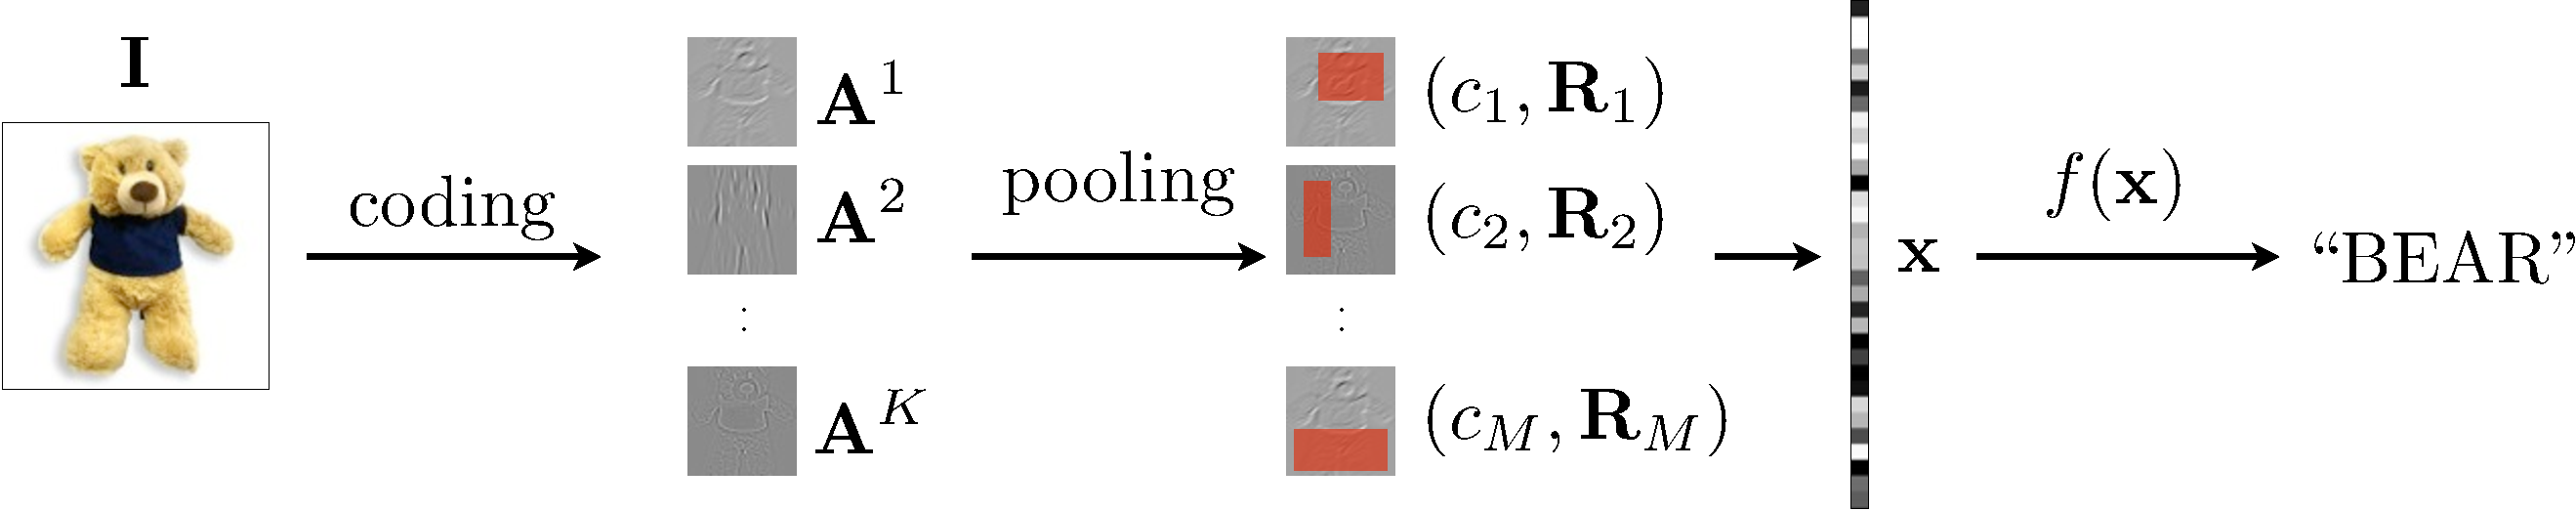
\includegraphics[width=1.\textwidth]{figs/smartpooling/pipeline_cvpr.pdf}
  \caption{The image classification pipeline. See Section \ref{sec:pipeline} for details.}\label{fig:pipeline}
  \vspace{-0.15in}
\end{figure*}

Before the introduction of the proposed methods, we briefly review the image classification pipeline we adopted, which leads to the problem of learning the receptive fields for spatial pooling. Specifically, we will focus on two-layer classification approaches.

We illustrate the pipeline from raw images to the prediction of class labels in Figure \ref{fig:pipeline}. Specifically, starting with an input image $\bI$, two stages are usually adopted to generate the global feature, as we formally define below.

\paragraph{(1) Coding.} In the coding step, we extract local image patches, and encode each patch to $K$ activation values based on a codebook of size $K$ (learned via a separate dictionary learning step). These activations are typically binary (in the case of vector quantization) or continuous (in the case of e.g.\ sparse coding). It is generally believed that having an over-complete ($K \gg$ the dimension of patches) codebook while keeping the activations sparse helps classification, especially when linear classifiers are used in the later steps.

Recently, Coates et al.~\cite{coates2011icml} have shown that relatively simple dictionary learning and encoding approaches lead to surprisingly good performances. To learn a dictionary $\bD =[\bd_1,\bd_2,\cdots,\bd_K]$ of size $K$ from randomly sampled patches $\{\bp_1,\bp_2,\cdots,\bp_N\}$ each reshaped as a vector of pixel values, two simple yet effective approaches are advocated:
\begin{enumerate}
  \item K-means, which minimizes the squared distance between each patch and its nearest code: $\min_{\bD} \sum_{i=1}^{N}\min_{j}\|\bp_i - \bd_j\|_2^2$.
  \item OMP-M, which learns a dictionary that minimizes the reconstruction error, with the constraint that each patch is modeled by a linear combination of at most $M$ codes: $\min_{\bD,\balpha_{i}} \sum_{i=1}^{N}\|\bp_i-\bD\balpha_i\|^{2}_{2}$, where the length of each dictionary entry $\bd_j$ is $1$, and the cardinality of each reconstruction coefficient $\balpha_i$ is at most $M$.
\end{enumerate}
For encoding, Coates et al.\ also propose to substitute sparse coding by the following efficient approaches:
\begin{enumerate}
  \item Triangle coding \cite{coates2010aistats}, which computes the activation of code $k$ for a patch $\bp$ as $f_k(\bx) = \max\{0,\mu(\bz) - z_k\}$, where $z_k$ is the distance from $\bp$ to the $k$-th code $\bd_k$, and $\mu(\bz)$ is the mean of distances from $\bp$ to all codes. 
  \item Soft thresholding, which computes the inner product between $\bp$ and each code, with a fixed threshold parameter $\alpha$: $f_{k}(\bx) = \max\{0, \bd_k^\top\bp - \alpha\}$
\end{enumerate}

We refer to \cite{coates2011icml} for a systematic discussion about different dictionary learning and encoding algorithms. In our experiment, we will adopt these standard approaches in order to isolate  the contribution of spatial pooling from the choice of different coding methods. Since local patches are usually extracted densely in a grid-based fashion, we will organize the activations of image $\bI$ as a set of matrices denoted by $\{\bA^{1}(\bI)\bA^{2}(\bI),\cdots,\bA^{K}(\bI)\}$, one for each code in the codebook, whose element $A_{ij}^k(\bI)$ contains the activation of code $\bd_k$ for the local image patch at spatial location $(i,j)$. 

\paragraph{(2) Pooling.} Since the coding result are highly over-complete and highly redundant, the pooling layer aggregates the activations over certain spatial regions of the image to obtain an $M$ dimensional vector $\bx$ as the global representation of the image. Each dimension of the pooled feature $\bx_i$ is obtained by taking the activations of one code in a specific spatial region (shown as the red rectangular in Figure \ref{fig:pipeline}), and performing a predefined operator (usually average or max) on the set of activations. 

We follow a similar approach to that in \cite{Boureau:2011tz} to formally define pooled features. Specifically, given an operator $\operatorname{op}$ that maps a set of real values to a single real value (e.g.\ by taking their average), a pooled feature $x_i$ can be defined based on the selection of a code indexed by $c_i$ and a spatial region denoted by $\bR_{i}$:
\begin{equation}
  x_i = \operatorname{op} (\bA^{c_i}_{\bR_{i}})
\end{equation}
Borrowing the definition from neuroscience, we call $\bR_i$ the \emph{receptive field} for the pooled feature, which could be seen as a binary mask over the image. $\bA^{c_i}_{\bR_{i}}$ is then the set of activations of code $c_i$ in the receptive field $\bR_i$.

This definition provides a general definition that embraces existing pooling algorithms. For example, commonly used operators involve computing the statistics of the activations under the $p$-norm:
\begin{equation}
  x_i = \frac{1}{|\bR_{i}|}(\sum\nolimits_{\alpha_i \in \bA^{c_i}_{\bR_{i}}} \alpha_i^{p})^{\frac{1}{p}}
\end{equation}
when $p=1$ this corresponds to the average pooling, and when $p\rightarrow \infty$ this corresponds to the max pooling.

We focus on the definition of receptive fields for pooling. The simplest form of pooling takes the whole image as the receptive field, thus assuming a bag-of-words model where spatial information is ignored. The more commonly adopted spatial pooling approach \cite{lazebnik2006beyond,Yang:2009vb} pools features from multiple levels of regular grids, thus defining a pyramid of pooled features. Given a set of $K$ codes and a set of $N$ receptive fields, the pooled features are then defined by taking the Cartesian product of the codes and the receptive fields, yielding a $KN$-dimensional global feature.

Finally, a classifier, usually linear SVM or logistic regression, is trained using the global feature vector to predict the final label of the image as $y = f(\bx;\btheta)$.

\section{Receptive Field Learning for Pooled Image Features}\label{sec:grafting}
While significant efforts have been placed on the coding part of the classification pipeline, the pooling step has received relatively little attention. Existing research on pooling mainly focuses on the analysis of the pooling operator, such as in \cite{Boureau:2010wz}. Specifically, spatial regions are almost always defined on regular grids \cite{Yang:2009vb}, which may not guarantee to be optimal. As a simple example, to distinguish most indoor and outdoor scenes, a human may look for the existence of the horizon, which could be captured by thin horizontal pooling regions over the image. Spatial grids, even with a pyramid structure, fail to provide such information. Such receptive fields may be dataset-dependent, leading us to ask the question \emph{``are spatial pyramids optimal for image classification?''}, the answer to which is often neglected by existing algorithms.

Instead of arbitrarily defining heuristic receptive fields, we aim to explicitly learn the receptive fields for classification tasks. Specifically, we propose to adaptively learn such regions by considering the receptive fields additional parameters, and jointly learning these parameters with the subsequent classifiers. The resulting benefit is two-fold: receptive fields tailored to classification tasks increase the overall accuracy of classification; in addition, with the help of such mid-level features, we are able to use a much lower-dimensional feature to achieve the state-of-the-art performance. We experiment with our algorithm on the benchmark CIFAR-10 dataset and other datasets, and report a significant improvement in both accuracy and efficiency.

Inspired by the selectivity of complex cells in the visual cortex, we propose to learn the pooled features adaptively. Specifically, learning a set of $M$ pooled features is equivalent to learning the parameters $\mathcal{C} = \{c_1,c_2,\cdots,c_M\}$ and $\mathcal{R} = \{\bR_1,\bR_2,\cdots,\bR_M\}$ \footnote{For simplicity, we will use the $\max$ operator, but note that any operator could also be incorporated in our framework.}. To this end, we note that the pooled features are directly fed into the final classifier, and propose to jointly learn the classifier parameters $\btheta$ together with the pooling parameters. Thus, given a set of training data $\mathcal{X} = \{(\bI_n,\by_n)\}_{n=1}^{N}$, the joint learning leads to solving the following optimization problem:
\begin{eqnarray}\label{eqn:adaptiverecfield}
  \min_{\mathcal{C},\mathcal{R},\btheta} & & \frac{1}{N}\sum_{n=1}^{N}\mathcal{L}(f(\bx_n;\btheta),\by_n) + \lambda\operatorname{Reg}(\btheta)\\
  \text{where} & & x_{ni} = \operatorname{op} (\bA^{c_i}_{n,\bR_{i}})\nonumber
\end{eqnarray}
where we assume that the coding from $\bI_{n}$ to $\{\bA^{c_i}_{n}\}_{i=1}^{K}$ is done in an unsupervised fashion, as has been suggested by several papers such as \cite{coates2010aistats}. We call this method receptive field learning, as the receptive fields are learned in such a way that information most relevant to the classification task will be extracted.

One practical issue is that solving the optimization problem (\ref{eqn:adaptiverecfield}) may be impractical, as there is an exponential number of receptive field candidates, leading to a combinatorial problem. Numerical solutions are also difficult, as the gradient with respect to the pooling parameters is not well-defined. Thus, instead of searching in the space of all possible receptive fields, we adopt the idea of over-completeness in the sparse coding community. Specifically, we start from a set of reasonably over-complete set of potential receptive fields, and then find a sparse subset of such pooled features. The over-completeness enables us to maintain performance, while the sparsity allows us to still carry out classification efficiently during testing time.

\begin{figure}
  \centering
  \begin{tabular}{ccc}
    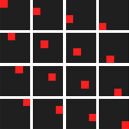
\includegraphics[width=0.27\linewidth]{figs/smartpooling/basebins.png} & %
    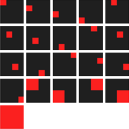
\includegraphics[width=0.27\linewidth]{figs/smartpooling/spmbins.png} & %
    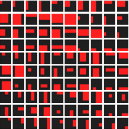
\includegraphics[width=0.27\linewidth]{figs/smartpooling/ocbins.png}\\
    (a) & (b) & (c)
  \end{tabular}
  \caption{An example of over-complete rectangular bins based on a $4\times 4$ super-pixel setting: (a) super-pixels; (b) spatial pyramid bins; (c) over-complete rectangular bins.}\label{fig:ocbins} 
\end{figure}

\subsection{Over-complete Receptive Fields}
The exponential number of possible receptive fields arises when we consider the inclusion and exclusion of single pixels individually. In practice this is often unnecessary, as we expect the active pixels in a receptive field to be spatially contiguous. In this work, we use receptive fields consisting of rectangular regions\footnote{As a side note, we also experimented with receptive fields that are sampled from an Ising model on the fly during training, but rectangular regions worked empirically better, possibly because the additional flexibility of Ising models leads to over-fitting the training data, and the spatial inconsistency may render randomly sampled receptive fields not as useful in classification tasks.}: this provides us a reasonable level of over-completeness, as there are $O(n^4)$ different rectangular receptive fields for an image containing $n\times n$ pixels. In addition, since the motivation of spatial pooling is to provide tolerance to small spatial displacements, we build the rectangular regions upon super-pixels, which are defined as dense regular grids on the image. Figure \ref{fig:ocbins} shows an example of such rectangular receptive fields compared with regions defined by the spatial pyramid on a $4\times4$ grid.

Given the set of $P$ over-complete regions, which we denote by $\mathcal{R} = \{\bR_{1},\bR_{2},\cdots,\bR_{P}\}$, and the dictionary $\mathcal{D} = \{\bd_1,\bd_2,\cdots,\bd_K\}$ of size $K$, we can define a set of $PK$ potential pooled features based the Cartesian product $\mathcal{R}\times\mathcal{D}$. Specifically, the $i$-th receptive field and the $j$-th code jointly defines the $(K\times i + j)$-th pooled feature as $x_{K\times i + j} = \operatorname{op} (\bA_{\bR_i}^{j})$. Note that when the coding and pooling are both carried out in an over-complete fashion, the resulting pooled feature is usually very high-dimensional.

\subsection{Structured Sparsity for Receptive Field Learning}
While it is possible to train a linear classifier using the high-dimensional pooled feature $\bx$ above, in practice it is usually beneficial to build a classifier using relatively low-dimensional features. In addition, for multiple-label classification, we want the classifiers of different labels to share features. This brings two potential advantages: feature computation could be minimized, and sharing features among different classifiers is known to provide robustness to the learned classifiers. To this end, we adopt the idea of structured sparsity \cite{quattoni2008transfer,schmidt2008structure}, and train a multiple-class linear classifier $\by = f(\bx) = \bW\bx + \bb$ via the following optimization problem:
\begin{equation}\label{eqn:structuredsparsity}
  \min_{\bW,\bb} \quad \frac{1}{N}\sum_{n=1}^{N}l(\bW^\top\bx_n+\bb, \by_n) + \frac{\lambda_1}{1}\|\bW\|_{\mathrm{Fro}}^{2} + \lambda_2\|\bW\|_{1,\infty}
\end{equation}
where $\by_i$ is the $L$-dimensional label vector coded in a $1-of-L$ fashion, with values taken from $\{-1,+1\}$ given $L$ classes. $\bx_i$ is an $M$-dimensional feature vector defined by over-complete pooling in the previous subsection, and $\bW = [\bw_1,\bw_2,\cdots, \bw_L]$ is a $M\times L$ weight matrix containing the weight vector for the $L$ classifiers. 

Two regularization terms are adopted in the optimization. The squared Frobenius norm $\|\bW\|_{\mathrm{Fro}}^2$ aims to minimize the structured loss in the classical SVM fashion, and the second regularizer is the $L_{1,\infty}$ norm of the matrix $\bW$:
\begin{equation}
  \|\bW\|_{1,\infty} = \sum_{i=1}^{M} \|\bW_{i,\cdot}\|_{\infty} = \sum_{i=1}^{M}\max_{j\in\{1,\cdots,L\}} |W_{ij}|
\end{equation}
where $\bW_{i,\cdot}$ denotes the $i$-th row of the matrix $W$. This regularizer introduces structured sparsity by encouraging the weight matrix $\bW$ to be row-wise sparse, so that the classifiers for different classes tend to agree on whether to use a specific feature, and when combined together, only jointly use a subset of the over-complete pooled features. The addition of the $L_{1,\infty}$ norm also provides a elastic-net like regularization, which is known to perform well when the dimension of data is much higher than the number of data points \cite{zou2005regularization}.

For optimization considerations, we use the multi-class extension of the binomial negative log likelihood (BNLL) loss function \cite{Perkins:2003vc}:
\begin{equation}
  l(\bW^\top\bx + \bb, \by) = \sum_{i=1}^{L}\ln(1+e^{-\by_i(\bW_{\cdot,i}^\top \bx + b_i)})
\end{equation}
The choice of the BNLL loss function over the hinge loss is mainly for computational simplicity, as the gradient is easier to compute for any input. In practice, the performance does not change much if we use the hinge loss instead.

\section{Fast Approximate Learning with Feature Grafting}
Jointly optimizing (\ref{eqn:structuredsparsity}) is still a computationally challenging task despite its convexity, due to the over-completeness in both coding and pooling. While it is possible to carry out the computation on smaller-scale problems like Caltech-101, we adopt a greedy approach to train the model for larger-scale problems. Inspired by the matching pursuit algorithm in dictionary training and the grafting algorithm \cite{Perkins:2003vc} in machine learning, we start with an empty set of selected features, incrementally add features to the set, and retrain the model when new features are added. 

\begin{figure}
  \centering
  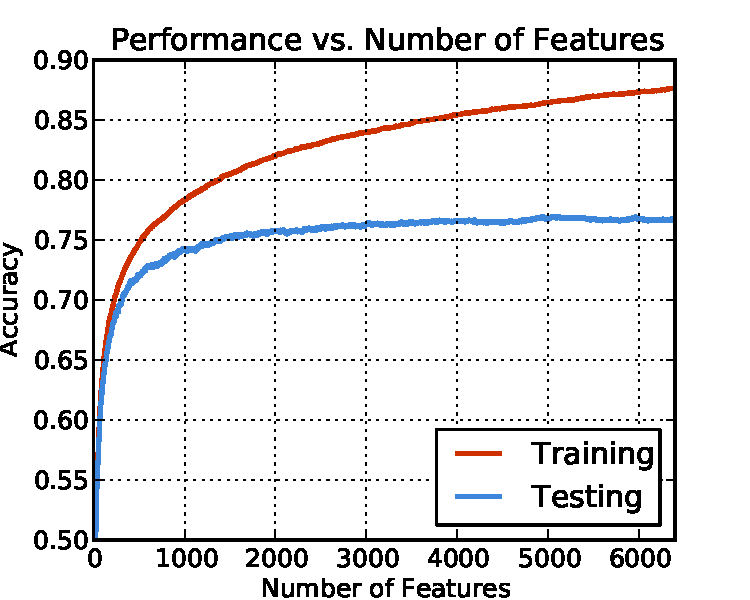
\includegraphics[width=0.5\textwidth]{figs/smartpooling/grafting_perf.pdf}
  \caption{Performance vs.\ number of selected features, with the experiment setting in Table \ref{table:gridsize} of Section \ref{sec:experiments}.}\label{fig:graftingsteps}
\end{figure}

Mathematically, we maintain a set $\mathcal{S}$ recording the set of currently selected features. At each iteration, for each feature index $j$ that has not been not selected, we compute the score of the feature as the 2-norm of the gradient of the objective function (\ref{eqn:structuredsparsity}), denoted by $\Loss(\bW,\bb)$, with respect to the corresponding weight vectors:
\begin{eqnarray}
  \operatorname{score}(j) = \left\|\frac{\partial \Loss(\bW,\bb)}{\partial \bW_{j,\cdot}}\right\|_\mathrm{Fro}^2
\end{eqnarray}

We then select the feature with the largest score, and add it to the selected set $\mathcal{S}$. The model is retrained using the previously learned optimum solution as the starting point. From a boosting perspective, this can be considered as incrementally learning weak classifiers, but our method differs from boosting in the sense that the weights for already selected features are also updated when new features are selected.

As the speed of retraining drops when more features are added, we adopt an approximate retraining strategy: for each iteration $t$, we select an active subset $\mathcal{S}_{A}$ of $\mathcal{S}$ based on the score above. We then retrain the model with respect to the active set and the bias term only:
\begin{equation}
  \bW^{(t+1)}_{\mathcal{S}_A,\cdot}, \bb = \operatorname{\arg\min}_{\bW_{\mathcal{S}_A,\cdot},\bb}\Loss(\bW,\bb)
\end{equation}
with the constraint that $\bW_{\bar{\mathcal{S}_A},\cdot}$ keep unchanged. The intuition is that with an already trained classifier from the previous iteration, adding one dimension will only introduce small changes to the existing weights. 

In practice, we found the performance of this approximate algorithm with the active set size less than 100 to be very close to the full retraining algorithm with a significant increase in computation speed. Figure \ref{fig:graftingsteps} shows typical curves of the training and testing accuracy with respect to the number of iterations. The performance usually stabilizes with a significantly smaller number of features, showing the effectiveness of introducing structured sparsity into classifier learning.

\section{Experiments}\label{sec:experiments}
We will mainly report the performance of our algorithm on the CIFAR-10 dataset\footnote{http://www.cs.toronto.edu/~kriz/cifar.html}, which contains 50,000 $32\times32$ images from 10 categories as training data, and 10,000 images as testing data.

We fix the dictionary learning algorithms to k-means clustering and the coding algorithms to triangular coding as proposed in \cite{coates2010aistats} for CFAR-10. Such a coding strategy has been shown to be particularly effective in spite of its simplicity. We also tested alternative dictionary learning and coding algorithms, which led to similar conclusions. As our main focus is on learning receptive fields for pooled features, the results of different coding algorithms are omitted, and we refer to \cite{coates2011icml} for a detailed discussion about dictionary learning and coding algorithms. 

For classification, when we use pre-defined receptive fields such as spatial pyramids, the SVM regularization term is chosen via 5-fold cross validation on the training data. When we perform feature selection, we fix $\lambda_1 = 0.01$ (which is the best value when performing 5-fold cross validation for max pooling on a 2$\times$2 regular grid) and drop $\lambda_2$, since the incremental feature selection already serves as a greedy approximation of the sparse constraint. Although the parameters are not tuned specifically for each configuration, we found it to perform well empirically under various scenarios.

\subsection{Spatial Pyramid Revisited}
It is interesting to empirically evaluate the performance of spatial pyramid regions against other choices of receptive fields. To this end, we trained a dictionary of size 200 (for speed considerations), and tested the performance of 3-layer spatial pyramid pooling against two algorithms based on over-complete receptive fields: (1) random selection from the over-complete pooled features, and (2) our method, both selecting the same number of features that spatial pyramid pooling uses. Results are shown in Figure \ref{fig:spmvsrandomvsgraft}. Our method outperforms SPM, but a more interesting finding is that the predefined spatial pyramid regions perform consistently worse than random selection, indicating that arbitrarily defined pooled features may not capture the statistics of real-world data well. With explicit learning of the pooling parameters, we achieved the highest performance among the three algorithms, showing the effectiveness and necessity of learning adaptive receptive fields.

\begin{figure}
  \centering
  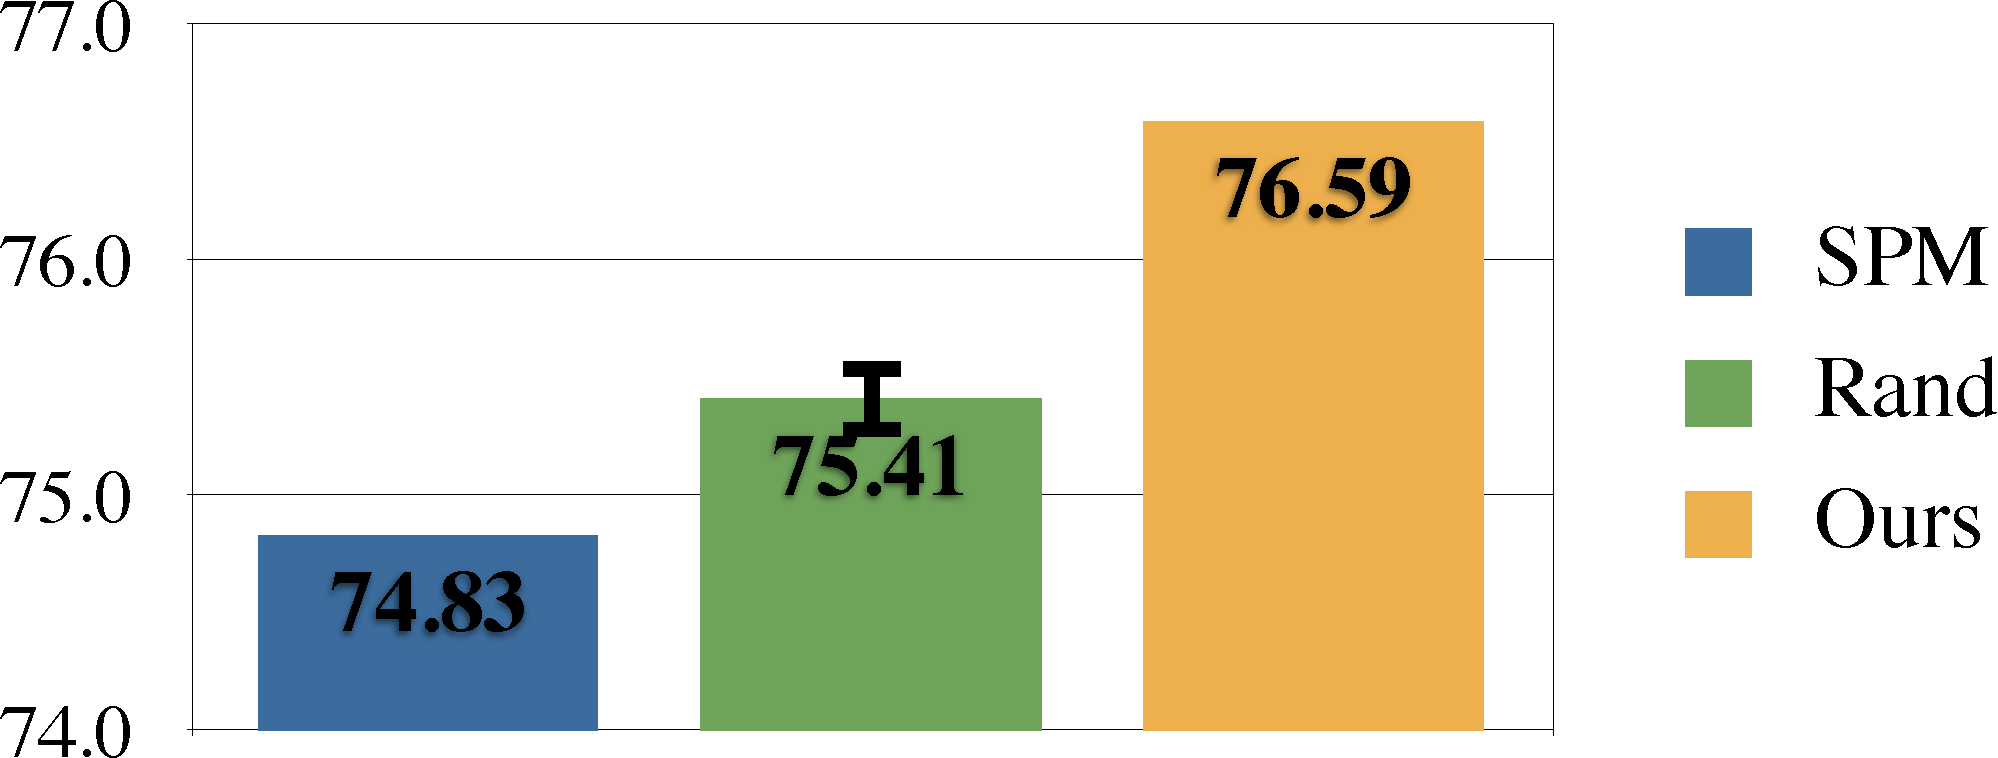
\includegraphics[width=0.5\textwidth]{figs/smartpooling/perfcomparison.pdf}
  \caption{Performance comparison among spatial pyramid pooling, random feature selection and our method, all using the same number of features for the final classification. It can be observed that a few selected features could already achieve a comparatively high performance.}\label{fig:spmvsrandomvsgraft}
\end{figure}

\subsection{The Effect of Spatial Over-completeness}

One may ask if the performance increase could be obtained without over-completeness by simply using a denser grid. To answer this question, we examined the performance of our algorithm against the 2$\times$2 pooling grid (which is used in \cite{coates2011icml} to obtain very high performance) and a denser $4\times4$ grid, associated with either average or max pooling. We also compared our method against random feature selection from the same pooling candidates. Table \ref{table:gridsize} summarizes the testing accuracy under various experimental settings, using a codebook size of 200.

Results from Table \ref{table:gridsize} demonstrates that denser pooling does help performance. The 4$\times$4 grid increases the performance by about 3 percent compared to 2$\times$2 pooling. However, with over-complete receptive fields we can almost always increase performance further. We achieved an 76.72\% accuracy with only 200 codes, already close with state-of-the-art algorithms using much larger codebook sizes (Table \ref{table:cifar10}). It is also worth pointing out that even random feature selection gives us comparable or better performance when compared to pre-defined pooling grids under the same number of feature dimension (e.g.\ compare the performance between $4\times4$ max pooling and randomly selecting $3,200$ features from an over-complete set of pooled features). 

Further, the importance of feature selection lies in two aspects: first, simply using all the features is not practical during testing time, as the dimension can easily go to hundreds of thousands when we increase the codebook size. Feature selection is able to get very close performance compared to using all the features, but with a significantly lower dimensionality, which is essential in many practical scenarios. Usually, feature selection enables us to achieve a high performance with only a few features (Figure \ref{fig:graftingsteps}). Adding remaining features will only contribute negligibly to the overall performance. Second, performing feature selection has the potential benefit of removing redundancy, thus increasing the generalization ability of the learned classifiers \cite{Perkins:2003vc,tibshirani1996regression}. In our experiment in Table \ref{table:gridsize}, the best performance is achieved with a few thousands features. Similarly, we found that with larger codebook sizes, using all the over-complete pooled features actually decreases performance, arguably due to the decrease of the generalization ability. 

% Notes: In case you are wondering, these numbers are obtained using the same codebook. It is run on the NEC skyservers, and the codebook is stored in the git repository logs/codebooks/200.mat.
\begin{table}
  \centering
  \begin{tabular}{r|r|r|c}
    \hline
    Pooling Area & Method & Features & Accuracy\\
    \hline
    2$\times$2 & Ave & 800 & 70.24\\
    4$\times$4 & Ave & 3,200 & 72.24\\
    2$\times$2 & Max & 800 & 66.31\\
    4$\times$4 & Max & 3,200 & 73.03\\
    3-layer SPM & Max & 4,200 & 74.83\\ % training 82.54%
    \hline
    OC + feat select & Max & 800 & 73.42\\
                  &     & 3,200 & 76.28\\
                  &     & 4,200 & 76.59\\
                  &     & 6,400 & {\bfseries 76.72}\\
    \hline
    OC, all features & Max & 20,000 & 76.44\\ % training 0.91064
    OC + rand select & Max & 800 & 69.48\\ % standard deviation 0.3442
    OC + rand select & Max & 3,200 & 74.42\\ % standard deviation 0.21247
    OC + rand select & Max & 4,200 & 75.41\\ % standard deviation 0.159
    \hline
  \end{tabular}
  \caption{Comparison of different pre-defined pooling strategies and our method (over-complete (OC) + feature selection). Random selection from the same over-complete pooled features is also listed, showing the necessity of better receptive field learning.}\label{table:gridsize}
\end{table}

\subsection{Larger Codebook vs.\ Better Spatial Pooling}
Under the two-stage pipeline adopted in this work, there are effectively two possible directions to increase the performance: to increase the codebook size and to increase the pooling over-completeness. We argue that these two directions are complementary: the performance gain from our effort on pooling could not simply be replaced by increasing the codebook size, at least not easily. More importantly, as the codebook size grows larger, it becomes more difficult to obtain further performance gain, while it is still relatively easy to obtain gains from better pooling.

To empirically justify this argument, we trained multiple codebooks of different sizes, and compared the resulting accuracies with and without over-complete pooling in Figure \ref{fig:ocpooling}. As can be observed, it becomes harder to obtain further performance gain by increasing the codebook size when we already have a large codebook, while using a better pooling strategy always brings additional accuracy gains. In fact, with our method, we are able to use a codebook of half the size (and half the number of pooled features) while maintaining performance (compare the green and blue curves). It is particularly interesting that, by selecting more features from the over-complete spatial regions, we are able to achieve state-of-the-art performance with a much smaller number of codes (the red curve), which has the potential in time-sensitive or memory-bounded scenarios.

\begin{figure}
  \centering
  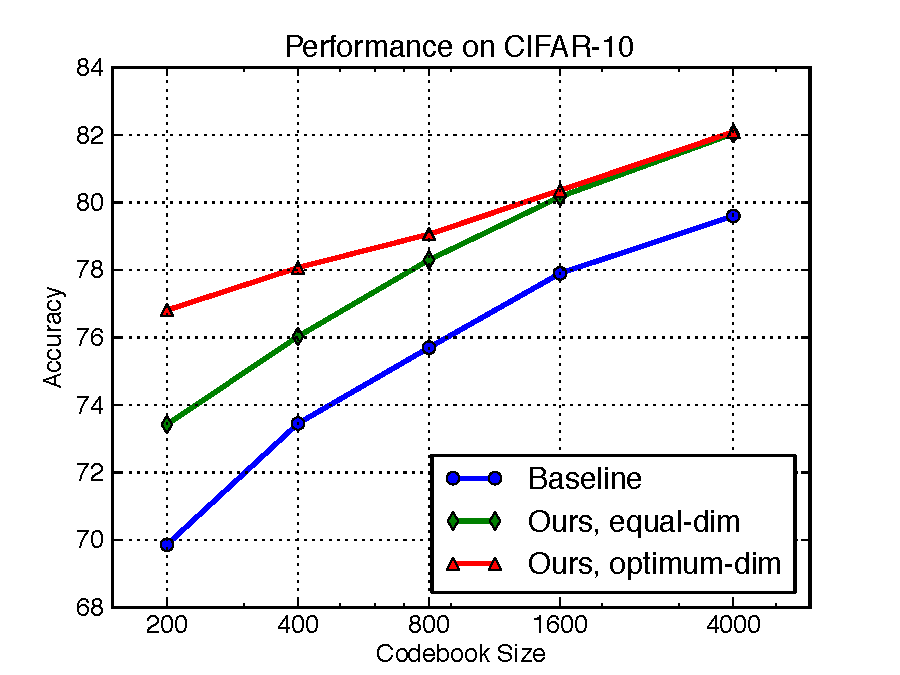
\includegraphics[width=0.5\textwidth]{figs/smartpooling/perf_vs_codes.pdf}
  \caption{Testing accuracies on CIFAR-10 with and without over-complete pooling. In the figure, ``equal-dim'' selects the same number of features as the baseline (Coates et al.\cite{coates2010aistats}), and ``optimum-dim'' selects the optimum number of features determined by cross-validation. (X-axis in log scale)}
  \label{fig:ocpooling}
\end{figure}

\begin{table}
  \begin{minipage}[c]{1\linewidth}
  \begin{center}
  \begin{tabular}{c|r|c}
    \hline
    Method & Pooled Features & Accuracy \\
    \hline
    ours, d=1600 & 6,400 & 80.17 \\
    ours, d=4000 & 16,000 & 82.04 \\
    ours, d=6000 & 24,000 & {\bfseries 83.11}\\
    \hline
    Coates et al. \cite{coates2010aistats}, d=1600 & 6,400 & 77.9\phantom{0} \\
    Coates et al. \cite{coates2010aistats}, d=4000 & 16,000 & 79.6\phantom{0} \\
    Coates et al. \cite{coates2011icml}, d=6000 & 48,000 & 81.5\phantom{0}\\
    \hline
    Conv. DBN \cite{Krizhevsky2010} & N/A & 78.9\phantom{0} \\
    Improved LCC \cite{Yu:2010wu} & N/A & 74.5\phantom{0} \\
    8-layer Deep NN \cite{2011arXiv1102.0183C} & N/A & 80.49 \\
    3-layer Deep NN \cite{coates2011selecting} & N/A & 82.0\phantom{0} \\
    \hline
  \end{tabular}
  \end{center}
  \end{minipage}
  \caption{Performance on the CIFAR-10 dataset. The first and second blocks compare performance between our method and Coates et al. \cite{coates2010aistats,coates2011icml} under similar codebook sizes, where the only difference is the spatial pooling strategy. The third block reports the performance of several state-of-the-art methods in the literature.}\label{table:cifar10}
\end{table}

\subsection{Best Performance}
Our best performance on the CIFAR-10 dataset was achieved by training a codebook size of 6,000, performing max pooling on over-complete rectangular bins based on a $4\times4$ grid, and selecting features up to 24,000 dimensions. We also note that the accuracy has not saturated at this number of features, but we would like to test the performance when the number of mid-level features is limited to a reasonable scale. With these settings, we achieved an accuracy of 83.11\% on the testing data. To the best of our knowledge, this is the best published result on CIFAR-10 without increasing the training set size by morphing the images. 

Table \ref{table:cifar10} lists the performance of several state-of-the-art methods. It is also worth pointing out that, to achieve the same performance, our algorithm usually uses a much lower number of features compared with other well-performing algorithms.

\subsection{Results on MNIST}
We can view the set of learned receptive fields for pooling as a saliency map for classification \cite{Itti:2001wa}. To visually show the saliency map and verify its empirical correctness, we applied our method to handwritten digit recognition on the MNIST dataset, on which convolutional deep learning models are particularly effective. To this end, we adopted a similar pipeline as we did for CIFAR-10: dense 6x6 local patches with ZCA whitening are used; a dictionary of size $800$ is trained with OMP-1, and thresholding coding with $\alpha=0.25$ (untuned) is adopted. The features are then max-pooled on over-complete rectangular areas based on a $6\times 6$ regular grid. Note that we used a different coding method from the CIFAR-10 experiment to show that the over-complete spatial pooling method is agnostic of the choice of low-level coding algorithms. Any parameter involved in the pipeline such as SVM regularization weights is tuned on a random 50k/10k split of the training data.

Figure \ref{fig:mnist} shows the 1-vs-1 saliency maps between digits. It can be seen that by learning receptive fields, the classifier focuses on regions where the digits have maximal dissimilarity, e.g., the bottom part for 8 and 9, and the top part for 3 and 5, which matches our intuition about their appearances. For 10-digit classification, we achieved an error rate of $0.64\%$, on par with several state-of-the-art algorithms (Figure \ref{fig:mnist} left). A gap still exists between our method and the best deep-learning algorithm, and combining receptive learning with deeper structures is future work.

\begin{figure}
  \centering
  \begin{minipage}[h]{0.4\linewidth}
  \centering
  \begin{tabular}{c|c}
    \hline
    Method & err\%\\
    \hline
    Baseline \cite{coates2011icml}\footnote{Our implementation.} & 1.02\\
    {\bfseries Our Method} & {\bfseries 0.64}\\
    \hline
    Lauer et al. \cite{lauer2007trainable} & 0.83\\
    Labusch et al. \cite{labusch2008simple} & 0.59\\
    Ranzato et al. \cite{ranzato2007unsupervised} & 0.62\\
    Jarrett et al. \cite{jarrett09} & 0.53\\
    \hline
  \end{tabular}
  \end{minipage}\hspace{0.5in}%
  \begin{minipage}[h]{0.4\linewidth}
  \centering
  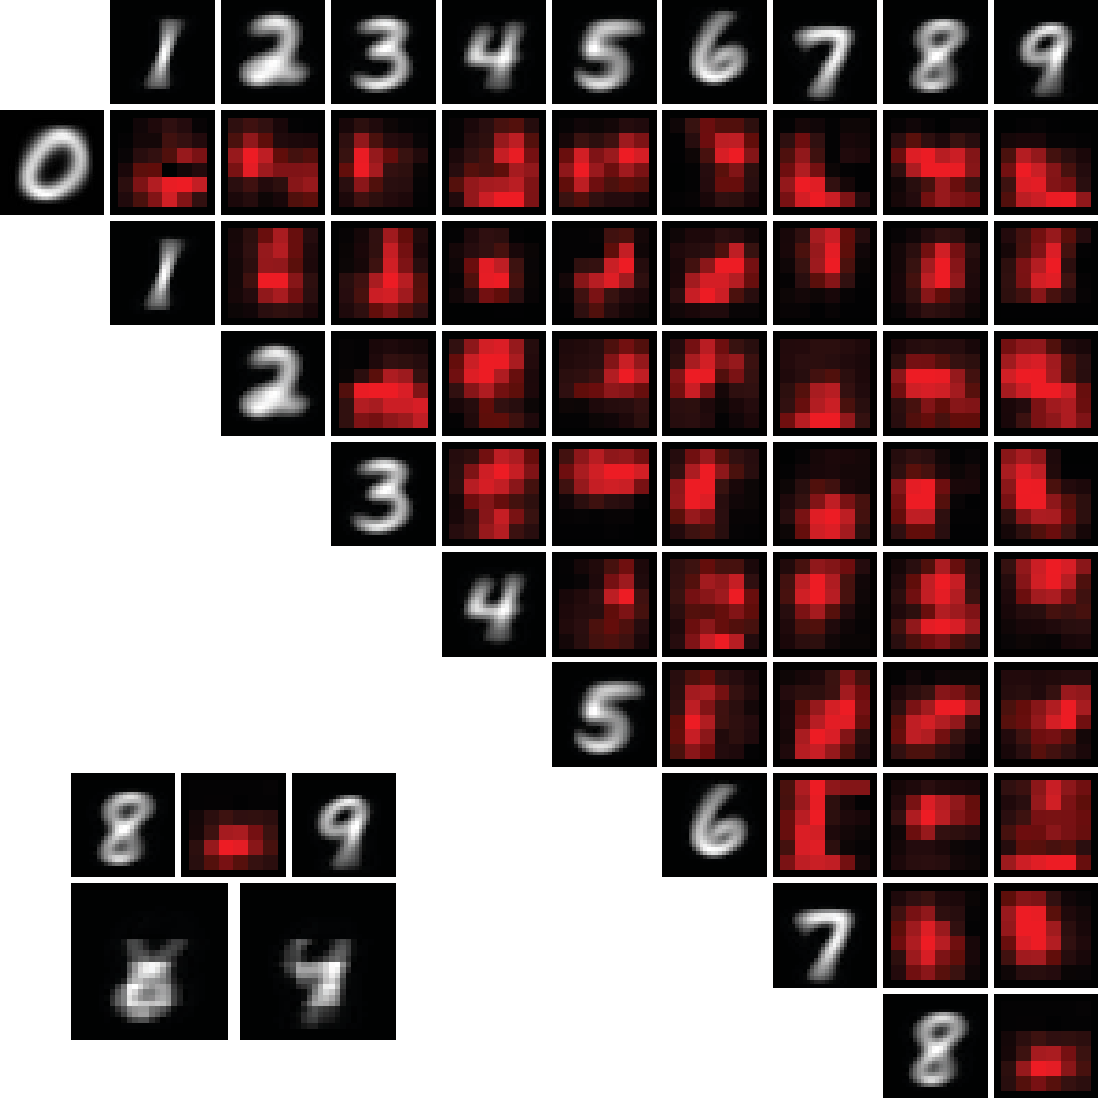
\includegraphics[width=1.\linewidth]{figs/smartpooling/saliency_mnist}
    \end{minipage}
  \caption{Left: Performance comparison (error rate in percentage) on MNIST. Top box: comparison between algorithms using similar pipelines. Bottom box: performance of other related algorithms in the literature. Right: 1-vs-1 saliency maps learned on MNIST. The left-bottom corner plots the mean of digit 8 and 9 multiplied by the corresponding saliency map, showing that the classifier focuses on the bottom part which intuitively also distinguishes the two digits best.}\label{fig:mnist}
\end{figure}

\begin{table}
  \centering
  \begin{tabular}{c|c|c|c}
    \hline
    Method & Codebook & Pooling & Performance\\
    \hline
    ScSPM \cite{Yang:2009vb} & 1024 (SC) & SPM & 73.2$\pm$0.54\\
    LCC+SPM \cite{wang2010locality} & 1024 & SPM & 73.44\\
    \bfseries{Our Method} & 1024 (SC) & OC & {\bfseries 75.3$\pm$0.70}\\
    Boureau et al. \cite{Boureau:2011tz} & 64K & SPM & 77.1$\pm$0.7\\
    \hline
  \end{tabular}
  \begin{tabular}{c|c}
    \hline
    SPM \cite{lazebnik2006beyond} & 64.6$\pm$0.7\\
    NBNN \cite{boiman2008defense} & 72.8$\pm$0.39 (15 training)\\
    Jarret et al. \cite{jarrett09} & 65.6$\pm$1.0\\
    RLDA \cite{Karayev2011RLDA} & 73.7$\pm$0.8\\
    Adaptive Deconv. Net \cite{zeileradaptive} & 71.0$\pm$1.0\\
    Feng et al. \cite{Feng:2011wv} & 82.6 \\
    \hline
  \end{tabular}
  \caption{Performance comparison (accuracy in percentage) on Caltech-101. Top: comparison between algorithms using similar pipelines. Bottom: performance of other related algorithms in the literature.}
  \label{tab:caltech}
\end{table}

\subsection{Results on Caltech-101}
Lastly, we report the performance of our algorithm compared with SPM on the Caltech-101 dataset in Table \ref{tab:caltech}. State-of-the-art performance following similar pipelines are also included in the table. Specifically, we used the same two-step pipeline as proposed by Yang et al. \cite{Yang:2009vb}: SIFT features are extracted from 16$\times$16 patches with a stride of 8, and are coded using sparse coding with a codebook of size 1024. For SPM, the coded features are pooled over a pyramid of $1\times1, 2\times2,4\times4$ regular grids; for a fair comparison we also use the $4\times4$ regular grid as our base regions, and select the same number of features as SPM uses.

As can be observed in the table, our pooling algorithm outperforms spatial pooling, although a gap still exists between our result and state-of-the-art methods, which uses more complex coding schemes than that we used. The results suggest that coding is a more dominant factor for the performance of Caltech-101. Existing research, especially the Naive Bayes nearest neighbor method \cite{boiman2008defense}, has also shown a consistent increase of accuracy with higher-dimensional coding output \cite{Boureau:2011tz,yang2010efficient}.
%\footnote{The recent work by Boureau et al. \cite{Boureau:2011tz} could be viewed from the coding perspective by mapping each patch onto the Cartesian space defined by two coding algorithms, and then doing normal spatial pooling to obtain the final global feature.}
However, we still obtain a consistent gain by adopting more flexible receptive fields for pooling, which justifies the effectiveness of the proposed algorithm. Note that the best performance reported by Feng et al. \cite{Feng:2011wv} was obtained by jointly learning the pooling operator ($p$ in $p$-norm pooling) and a per-code spatial saliency map in addition to a larger dictionary, which also follows the idea of learning better spatial information beyond SPM.


\subsection{Transferring Class-Independent Pooling Knowledge}
Beyond classifying existing labels during training, we are also interested in examining whether the learned receptive fields work equally well on unseen classes. While several papers have suggested that simplex cells in V1 performs sparse encoding independent from class labels, and that unsupervised feature learning performs well for the coding step, little is known about the pooling strategy. Learning class-independent pooling knowledge is closely connected to the visual attention model \cite{Itti:2001wa}, which answers the question ``what does an object look like in general''.

To examine the performance of our method against new classes, we utilize the CIFAR-100 dataset, which contains 100 categories with 500 training examples per class. We extract features in the same fashion, and train the SVM classifier with learned codes and receptive fields from CIFAR-10. The classification result is compared against the accuracy rate obtained from directly learning the receptive fields on CIFAR-100, and a baseline that does random feature selection from the same set of over-complete features. For a fair comparison, all methods use a codebook size of 1,600 and select 6,400 dimensional features. We also tested learning pooled features on CIFAR-100 and testing on CIFAR-10, and the performances are reported in Table \ref{table:transfer}.

\begin{table}
  \centering
  \begin{tabular}{c|l|l}
    \hline
    Classification on & Feature Selection on & Accuracy \\
    \hline
          & CIFAR-10     & {\bfseries 54.88} \\ % training 89.14, reg 0.01
          & CIFAR-100      & 54.83\\ % training 92.39, reg 0.01
    CIFAR-100 %& 2x2 Max Pooling  & 47.26\\ % training 99.62, reg 0.01
          %& 2x2 Ave Pooling  & 47.01\\ % training 78.59, reg 0.001 
          & Random Selection & 54.48$\pm$0.25\\
    \hline
             & CIFAR-100    & 78.88 \\ % training 90.57, reg 0.01
             & CIFAR-10     & {\bfseries 80.17}\\ % reg 0.01
    CIFAR-10 %& 2x2 Max Pooling   & 75.28 \\ % training 86.07, reg 0.01
             %& 2x2 Ave Pooling   & 75.86 \\ % training 90.25, reg 0.0001
             & Random Selection & 78.95$\pm$0.20\\

    \hline
  \end{tabular}
  \caption{The performance of transferring pooled feature between CIFAR-10 and CIFAR-100 compared against natively learned features and random selection.}\label{table:transfer}
\end{table}

The result we obtained showed a mixed message. While the features are leaned from CIFAR-10, they perform well on the CIFAR-100 dataset, and the performance is even better than natively learned features. For the other direction, transferring learned features does not show a statistically significant difference compared with random selection. A possible explanation of such scenario may be that with less training data per class on CIFAR-100, the feature selection algorithm may suffer more from overfitting than it does on CIFAR-10, reducing the generalization ability of the learned features.

In general, our experiment does show the hope for a better and class-independent pooling strategy. Possible future work may involve utilizing larger-scale image databases, and exploring pooled feature learning in an unsupervised approach, which may further reveal valuable pooling strategies.

\section{Summary}

This chapter focused on analyzing the basic coding and pooling component of the state-of-the-art image feature extraction pipelines. Specifically, we show that smarter algorithms that explicitly take into consideration the pooling stage, whether to find better spatial receptive fields or to find pooling-aware lower level dictionaries, provide significant performance boosts in the final classification accuracies.

%\section*{Notes}
%
%Parts of this chapter have appeared in peer-reviewed publications as we list below:
%\begin{enumerate}
%\item Yangqing Jia, Chang Huang, Trevor Darrell. Beyond Spatial Pyramids: Receptive Field Learning for Pooled Image Features. CVPR 2012.
%\end{enumerate}

\chapter{Theoretical Analysis for Feature Learning}\label{chapter:nystrom}

\section{Size Matters: a Theoretical Analysis}

One important phenomenon observed in the above section (see \eg Table \ref{table:cifar10} and Figure \ref{fig:ocpooling}), as well as in related publications \cite{coates2010analysis,coates2011icml}, is that feature dimension almost always plays a key role in the final classification performance. With higher dimensional features and a simple linear classifier, performance usually appear to be monotonically increasing, although higher dimensionality comes with higher computational costs. It is also noteworthy that with a rather simple coding scheme and dictionary learning, results were in most cases comparable to the widely used but more computationally expensive sparse coding technique \cite{coates2011icml}. Furthermore, even selecting random dictionaries yielded close to state-of-the-art results. Further work on this domain \cite{freitas} suggests that the encoding technique used is a proxy to solving sparse coding (but in a simple and faster fashion).

The fact that random dictionaries perform well when operating with large codebook sizes poses interesting questions such as how feature size affects performance. In addition, even though the size of the dictionary (or codebook) is important, the accuracy seems to saturate, which is a phenomenon that was empirically verified in many tasks, and for which we now give a theoretical interpretation by linking random dictionaries with \nystrom sampling. In this section, we explain in detail how the feature learning approach could be viewed as a \nystrom sampling scheme from a high-dimensional (potentially infinite dimensional) feature space, and then derive proper bounds to model the behavior we observe in the classification experiments. We will use slightly different notations from the previous section, as we will focus on mathematics that is not necessarily binded to specific coding or pooling operations.

\subsection{The \nystrom Sampling View}
\nystrom sampling has been proposed as an efficient way to approximate large PSD matrices (such as kernel matrices) by sampling columns of the matrix. Specifically, let $\bK$ be an $N\times N$ matrix, the \nystrom method defines an approximation as $\bK' = \bE\bW^{+}\bE^\top$, where $\bE$ is a $N\times c$ matrix with the $c$ columns randomly sampled from those of $\bK$, and $\bW$ is the square $c\times c$ matrix formed by picking the same $c$ columns and rows from $\bK$. Such a sampling perspective have been shown to be very effective in kernel machines \cite{zhang2008improved,cortes10,kumar2012sampling}.

We consider forming a dictionary by sampling our training set (although, as discussed below, better techniques exist that lead to further gains in performance). To encode a new data point $\bx \in \mathbb{R}^d$, we apply a (generally non-linear) coding function $\bc$ so that $\bc(\bx) \in \mathbb{R}^c$. The standard classification pipeline considers $\bc(\bx)$ as the new feature space, and typically uses a linear classifier on this space. In this section, we consider the threshold encoding function as in \cite{coates2011icml}, $\bc(\bx) = \max(0,\bx^\top\bD - \alpha)$, but the derivations are valid for other different coding schemes.

In the ideal case (infinite computation and memory), we encode each sample $\bx$ using the whole training set $\bX \in \mathbb{R}^{d \times N}$, which can be seen as the best local coding of the training set $\bX$, to the extent that overfitting is handled by the classification algorithm. In fact, larger dictionary sizes yield better performance assuming the linear classifier is well regularized, as it can be seen as a way to do manifold learning \cite{wang2010locality}. We define the new features in this high-dimensional coded space as $\bC = \max(0,\bX^\top\bX - \alpha)$, where the $i$-th row of $\bC$ corresponds to coding the $i$-th sample $\bc(\bx_i)$. The linear kernel function between samples $i$ and $j$ is $K(\bx_i,\bx_j) = \bc(\bx_i)^\top\bc(\bx_j)$. Thus, performing linear classification on the coded features effectively uses the kernel matrix $\bK = \bC\bC^\top$.

In the conventional context of \nystrom sampling for kernels, one randomly samples a subset of the columns of $\bK$ and then replaces the original matrix $\bK$ with a low-rank approximation $\hat{\bK}$. However, in our problem, naively applying \nystrom sampling to the matrix $\bK$ does not save any computation, as every column of $\bK$ requires to encode the corresponding feature with the large dictionary of all $N$ samples. However, if we approximate the matrix $\bC$ with \nystrom sampling to obtain $\bC' \approx \bC$, we would get an efficient approximation of the kernel matrix as $\bK' \approx \bK$:
\begin{align}
\bC' & = \bE \bW^{-1} \bE^\top, \text{ and}\\
\bK' & = \bC' \bC'^\top = \bE \bW^{-1} \bE^\top \bE \bW^{-1} \bE^\top = \bE \bLambda \bE^\top,
\end{align}
where the first equation comes from applying \nystrom sampling to $\bC$, $\bE$ is a random subsample of the columns of $\bC$, and $\bW$ the corresponding square matrix with the same random subsample of both columns and rows of $\bC$.

We note that in the traditional coding scheme proposed in \cite{coates2011icml},  if the dictionary is taken randomly then $\bK_{coding} = \bE \bE^\top$, and by applying \nystrom sampling to $\bC$ we obtain almost the same kernel, where the matrix $\bLambda$ acts as an additional Mahalanobis metric on the coded space.
%eWe found the matrix $\bLambda$ to be strongly diagonal (even more so if instead of sampling, one tries to minimize the similarity between dictionary elements (such as in K-means)).
Adding the term $\bLambda$ seemed to help in some cases, when the dictionary size is small (for example, in the CIFAR10 dataset, classification performance was improved by about $0.5\%$ when $c<500$.). We refer to the supplementary material to discuss the effect of $\bLambda$ and how to efficiently find it without explicitly computing the original $N\times N$ matrix. 
%The conceptual diagram of the \nystrom sampling view can be seen in Figure \ref{fig:concept}.

\subsection{Error Bounds on the Approximation}

Many existing analyses have computed bounds on the error made in estimating $\bC$ by $\bC'$ by sampling $c$ columns, such as \cite{talwalkar2010matrix,kumar2012sampling}, but not between $\bK = \bC\bC^\top$ and $\bK'=\bC'\bC'^\top$, which we aim to analyze in this section. The bound we start with is \cite{kumar2012sampling}:
\begin{equation}
\label{eqn:nyst_bound}
||\bC-\bC'||_F \leq ||\bC-\bC_k||_F + \epsilon \max(n\bC_{ii}),
\end{equation}
valid if $c \geq 64k/\epsilon^4$ ($c$ is the number of columns that we sample from $\bC$ to form $\bE$, i.e. the codebook size), where $k$ is the sufficient rank to estimate the structure of $\bC$, and $\bC_k$ is the optimal rank $k$ approximation (given by Singular Value Decomposition (SVD), which we cannot compute in practice). %Note that, if we assume that our training set can be explained by a manifold of a certain dimension $k$ (i.e. the first term in the right hand side of Eqn.\ (\ref{eqn:nyst_bound}) vanishes), then the error is proportional to $\epsilon$ times a constant (that is dataset dependent).

Fixing $k$ to the value that retains enough energy from $\bC$, we get a bound that gives a minimum $\epsilon$ to plug in Eqn.\ \ref{eqn:nyst_bound} for every $c$ (sample dictionary size). This gives us a useful bound of the form $\epsilon \geq \hat{M}\left(\frac{1}{c}\right)^{\frac{1}{4}}$ for some constant $\hat{M}$ (that depends on $k$). Hence:
\begin{equation}
||\bC-\bC'||_F \leq O + M\left(\frac{1}{c}\right)^{\frac{1}{4}},
\end{equation}
where $O$ and $M$ constants that are dataset specific.

However, having bounded the error $\bC$ is not yet sufficient to establish how the code size will affect the classifier performance. In particular, it is not clear how the error on $\bC$ affect the error on the kernel matrix $\bK$. Similarly, having a kernel matrix of different quality will affect classification performance. Recent work \cite{cortes10} proves a linear relationship between kernel matrix degradation and classification accuracy. Furthermore, in the supplementary material, we provide a proof that shows the degradation of $\bK$ is also proportional to the degradation of $\bC$. Hence, the error bound on $\bK'$ is of the same form as the one we obtained for $\bC$:
\begin{equation}
||\bK-\bK'||_F \leq O' + M'\left(\frac{1}{c}\right)^{\frac{1}{4}}.
\label{eqn:bound}
\end{equation}

We briefly prove the bound here. Recall that $\bK = \bC\bC^\top$ and $\bK' = \bC'\bC'^\top$, and since $\bC$ and $\bC'$ are symmetric, $\bK = \bC^2$ and $\bK' = \bC'^2$. Note that the Frobenius norm satisfies subadditivity and submultiplicativity properties \cite{meyer01}, i.e.,
\begin{align}
    ||A+B||_F & \leq ||A||_F+||B||_F\text{, and}\\
    ||AB||_F & \leq ||A||_F||B||_F.
\end{align}
Thus, we have
\begin{align}
||\bK - \bK'|| & = ||\bC^2 - \bC'^2|| \\
& = ||(\bC-\bC')\bC + \bC'(\bC-\bC')|| \nonumber\\
& \leq ||(\bC-\bC')\bC|| + ||\bC'(\bC-\bC')||\nonumber\\
& \leq ||(\bC-\bC')||||\bC|| + ||\bC'||||(\bC-\bC')||\nonumber\\
& \leq ||(\bC-\bC')||||\bC|| + ||\bC'-\bC||^2 +\nonumber\\
& \phantom{\leq} + ||\bC||||(\bC-\bC')||\nonumber\\
& = ||(\bC-\bC')||\left(||(\bC-\bC')|| + 2||\bC||\right)\nonumber\\
& = \mathcal{O}(||(\bC-\bC')||)\nonumber
\end{align}
where all the $||.||$ are the Frobenius norms, and where in the last line we assumed that $||(\bC-\bC')||$ is sufficiently small and $||\bC||$ is constant w.r.t. $c$.  Thus, we can expect that the approximation quality of $\bK'$ will be similar than $\bC'$, and we will further assume that the quality of the kernel approximation $\bK'$ will determine the accuracy of the final classifier, which we will also empirically show in the experiments.

We note that the bound above also applies to the case when further steps, such as pooling, is carried out after coding, provided that such steps produce output feature dimensions that have a one-to-one correspondence with the dictionary entries. Pooling over multiple spatial regions does not change the analysis as it could be deemed as concatenating multiple kernel matrices for the data.

\begin{figure}
    \centering
    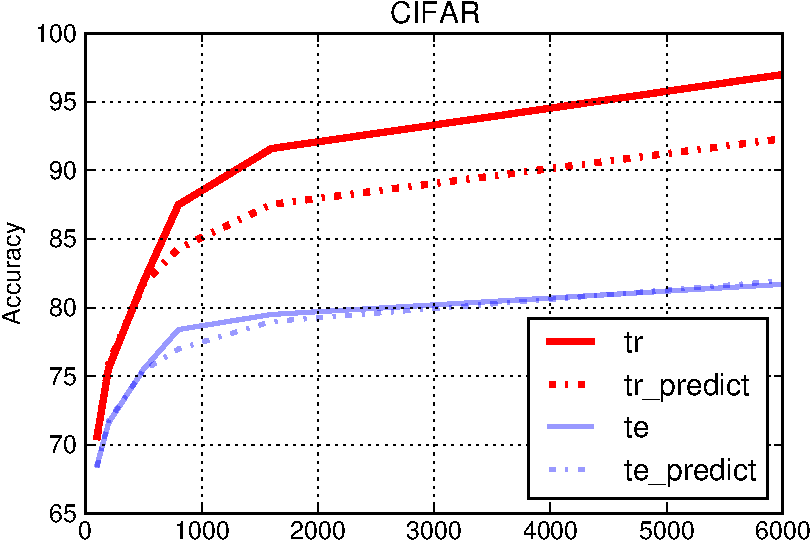
\includegraphics[width=0.4\textwidth]{figs/sizematters/bound_CIFAR.pdf}
    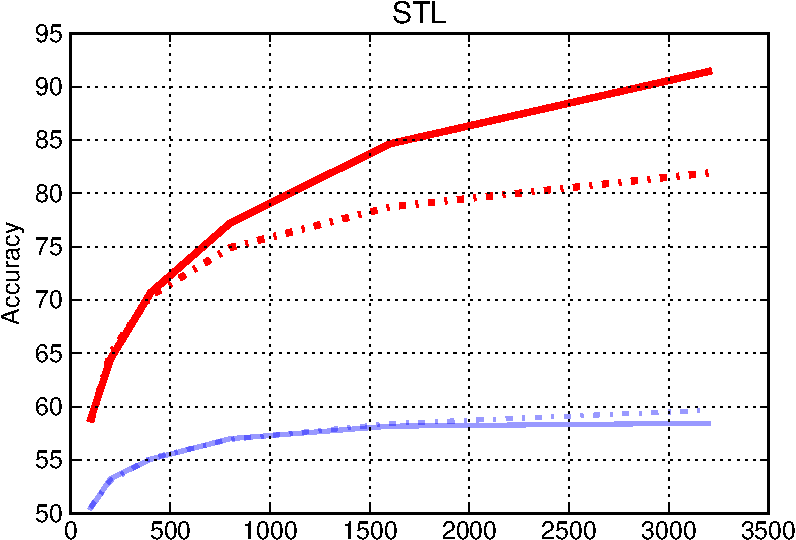
\includegraphics[width=0.4\textwidth]{figs/sizematters/bound_STL.pdf}
    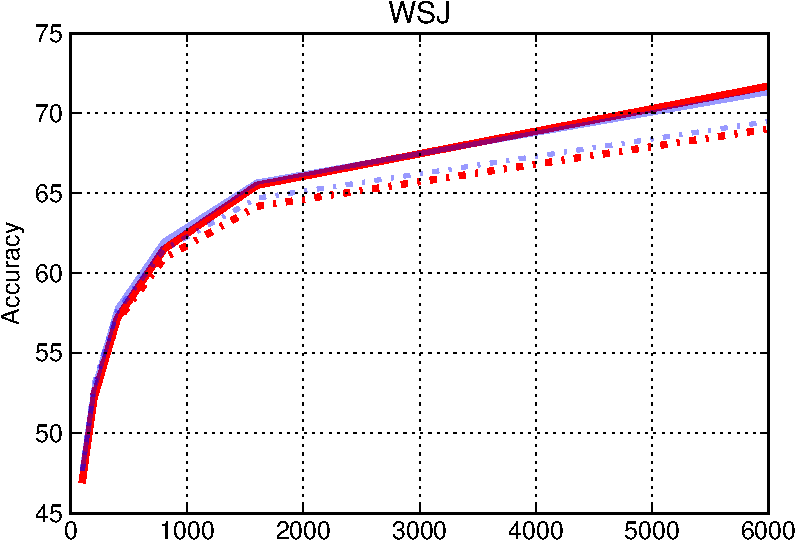
\includegraphics[width=0.4\textwidth]{figs/sizematters/bound_WSJ.pdf}
    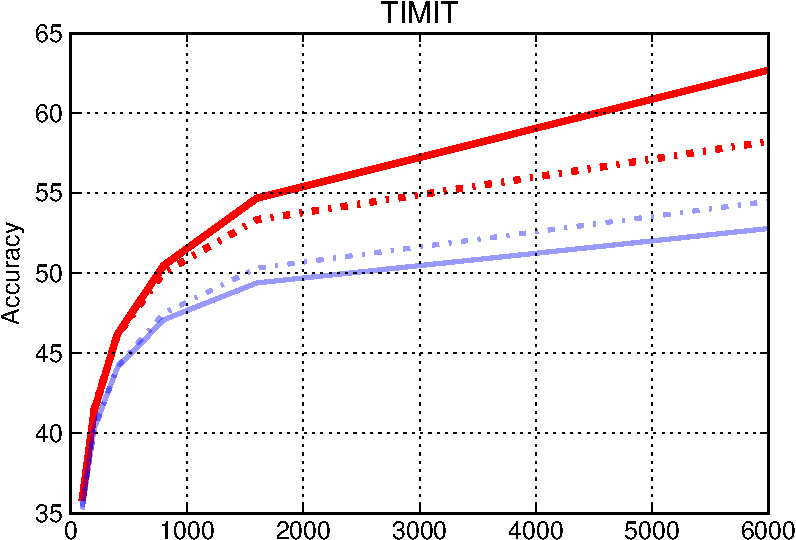
\includegraphics[width=0.4\textwidth]{figs/sizematters/bound_TIMIT.pdf}
    \caption{The actual training and testing accuracy (solid) and the predicted accuracy using our bound (dashed), on four datasets: CIFAR, STL, WSJ and TIMIT from left to right and top to bottom.}\label{fig:bounds}
\end{figure}

\subsection{Evaluating Bounds}
We empirically evaluate the bound on the kernel matrix, used as a proxy to model classification accuracy, which is the measure of interest. To estimate the constants in the bounds, we do interpolation of the observed accuracy using the first three samples of accuracy versus codebook size, which is of practical interest: one may want to quickly run a new dataset through the pipeline with small dictionary sizes, and then quickly estimate what the accuracy would be when running a full experiment with a much larger dictionary (which would take much longer to run) with our formulation. We always performed \nystrom sampling schemes by doing K-means instead of random selection (although the accuracy between both methods does not change too much when $c$ is sufficiently large).

In Figure \ref{fig:bounds} we plot the accuracy (on both train and test sets) on four datasets: CIFAR-10 and STL from vision, and WSJ and TIMIT from speech. For each dataset we used the first three samples to determine the constants given in the bound. One may practically favor this approach to evaluate performance, as small dictionary sizes are fast to try while large dictionary sizes are of interest. The bound is designed to predict training accuracy \cite{cortes10}, but we also do regression on testing accuracy for completeness. We note that testing accuracy will in general also be affected by the generalization gap, which is not captured by the bound analysis.

The results show that in all cases, the red dashed line is a lower bound of the training actual accuracy, and follows the shape of the empirical accuracy, predicting its saturation. In the testing case, our model is slightly optimistic when overfitting exists (e.g. STL and TIMIT), but correctly predicts the trend with respect to the number of dictionary entries.

The implication of linking \nystrom sampling theory to current learning pipelines has several immediate consequences: first, it clarifies why random sampling or K-means produce very reasonable dictionaries that are able to perform well in terms of classification accuracy \cite{zhang2008improved,coates2010aistats,kumar2012sampling}; more importantly, due to known bounds such as the one derived in this section, we can model how the codebook size will affect performance by running a few experiments with smaller codebook sizes, and extrapolating to larger (and more computationally expensive to compute) codebook sizes by means of Eq.~\ref{eqn:bound}, thus predicting accuracies before running potentially long jobs.

We further note that, although our experiment is carried out only by varying the number of codes in the dictionary (to better align speech and vision benchmarks), the pooling operation also falls under the same category: essentially, the whole coding + pooling pipeline could be viewed as a \nystrom sampling approach that samples features from the cartesian space of individial codes and individual pooling regions. Also, while we used the term ``sampling'', the actual feature selection does not necessarily have to be random: research in the \nystrom sampling methods suggests that more data-dependent feature selection approaches, notably K-means, works better than completely randomly sampling features \cite{zhang2008improved,kumar2012sampling}, while the theoretical bound still applies to these scenarios. Our work on selecting receptive fields aligns with such work, providing a more informed approach to find better pooled features for classification.

\section{PADL: Pooling Aware Dictionary Learning}\label{sec:sizematters:algorithm}

The \nystrom sampling view suggests that one could find a better subset of a large (potentially infinite) dictionary to obtain more informative features. In addition, existing work suggests that this could be often done in an efficient way with methods such as clustering. However, current clustering algorithms for dictionary learning \cite{coates2010aistats,coates2011icml} only apply to the local coding step, and do not consider the pooling effect. The \nystrom sampling insight suggests that simple feature selection approaches may exist that embraces more complex pipelines. As a concise example, we show that by explicitly taking into account the whole pipeline shown in Figure \ref{fig:pipeline} to include both local coding and pooling when learning the dictionary, one gets a much more compact feature representation.

Figure \ref{fig:feature_correlation} shows two examples why pooling-aware dictionary learning may be necessary, as local patch-based dictionary learning algorithms often yield similar filters with small translations. Such filters, even when uncorrelated on the patch level, produce highly correlated responses when pooled over a certain spatial region, leading to redundancy in the feature representation.

\begin{figure}
    \centering
    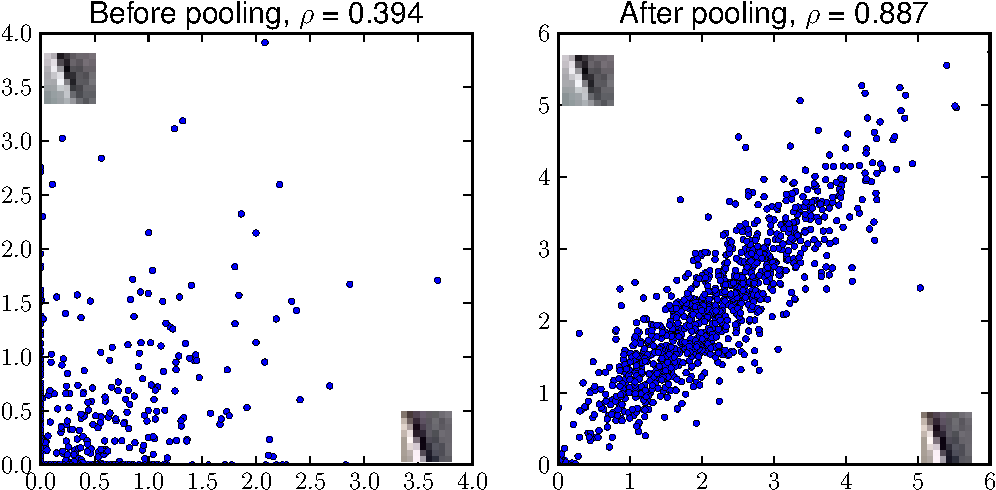
\includegraphics[width=0.7\linewidth]{figs/sizematters/distribution/12_distribution_final.pdf}\\
    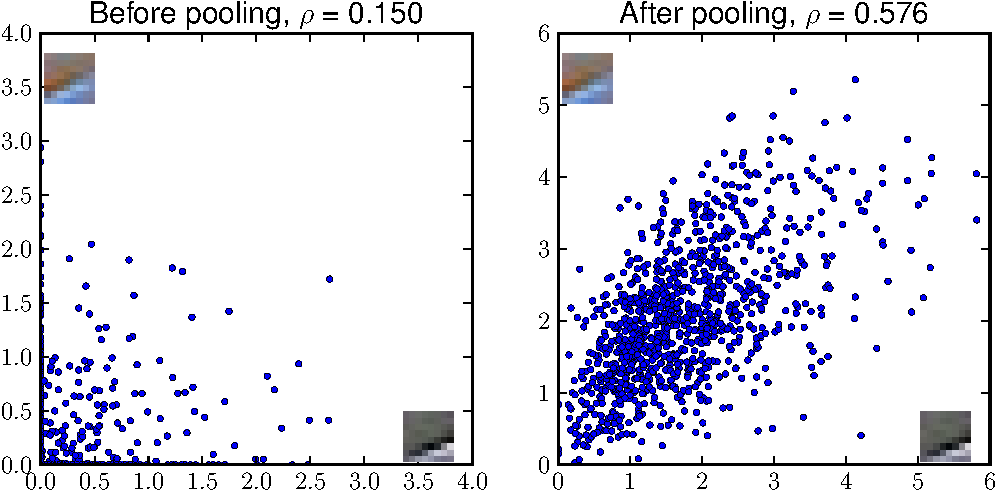
\includegraphics[width=0.7\linewidth]{figs/sizematters/distribution/34_distribution_final.pdf}
    \caption{Two codes learned from a patch-based K-means algorithm that produce lowly correlated patch-based responses (left), but highly correlated responses after pooling (right). Such phenomenon may root from various causes, such as codes with translational difference (above) and color difference (below).}\label{fig:feature_correlation}
\end{figure}

Observing the effectiveness of clustering methods in patch-based dictionary learning, we propose to learn a final dictionary of size $K$ in two stages: first, we adopt the K-means algorithm to learn a more over-complete starting dictionary of size $M$ ($M >> c$) on patches, effectively ``overshooting'' the dictionary we aim to obtain. We then perform encoding and pooling using the dictionary, and learn the final smaller dictionary of size $c$ from the statistics of the $M$-dimensional pooled features.

\subsection{Post-Pooling Feature Selection}
The first step of our algorithm is identical to the patch-based K-means algorithm with a dictionary size $M$. After this, we can sample a set of image super-patches of the same size as the pooling regions, and obtain the $M$ dimensional pooled features from them. Randomly sampling a large number of pooled features in this way allows us to analyze the pairwise similarities between the codes in the starting dictionary in a post-pooling fashion. We would then like to find a $c$-dimensional, lower dimensional subspace that best represents the $M$ pooled features.

If we simply would like to find a low-dimensional representation from the $M$-dimensional pooled features, one would naturally choose SVD to find the $K$ most significant projections of the covariance matrix. With a little abuse of terminology and denoting the matrix of randomly selected pooled feature as $\bX$ where each column is a feature vector, the SVD is carried out as
\begin{equation}
    \bX \approx \bU_c\bLambda_c\bV_c^\top,
\end{equation}
where $\bR$ is the covariance matrix computed using the random sample of pooled features, the $M\times c$ matrix $U_c$ contains the left singular vectors, and the $c\times c$ diagonal matrix $\bLambda_c$ contains the corresponding singular values. The low-dimensional features are then computed as $\bx_c = \bU_c^\top\bx$.

While the ``oracle'' low-dimensional representation by SVD guarantees the best $c$-dimensional approximation, it does not meet our goal since the dictionary size is not reduced, as SVD almost always yields non-zero coefficients for all the dimensions. Linearly combining the dictionary entries does not work either due to the nonlinear nature of the encoding algorithm. In our case, we would need the coefficients of only a subset of the features to be non-zero, so that a minimum number of filters need to be applied during testing time. Various machine learning algorithms aim to solve this, most notably structured sparse PCA \cite{jenatton2010structured}. However, these methods often requires a structured sparsity term to be applied during learning, making the training time-consuming and difficult to scale up.

Based on the analysis of the last section, the problem above could again be viewed as a \nystrom sampling problem by subsampling the rows of the matrix $\bX$ (corresponding to selecting codes from the large dictionary). Empirical results from the \nystrom sampling then suggests the use of clustering algorithms to solve this. Thus, we resort to a simpler K-centroids method.

Specifically, we use affinity propagation \cite{frey2007clustering}, which is a version of the K-centroids algorithm, to select exemplars from the existing dictionary. Intuitively, codes that produce redundant pooled output (such as translated versions of the same code) would have high similarity between them, and only one exemplar would be chosen by the algorithm. We briefly explain the affinity propagation procedure here: it finds exemplars from a set of candidates where pairwise similarity $s(i,j)$ ($1 \leq i, j \leq M$) can be computed. It iteratively updates two terms, the ``responsibility'' $r(i,j)$ and the ``availability'' $a(i,j)$ via a message passing method following such rules \cite{frey2007clustering}:
\begin{align}
    r(i,k) & \leftarrow s(i,k) - \max_{k'\neq k}\{a(i,k') + s(i,k')\}\label{ap:r}\\
    a(i,k) & \leftarrow \min\{0, r(k,k) + \sum\nolimits_{i'\notin\{i,k\}}\max\{0, r(i',k)\}\}\nonumber\\
           & \phantom{\leftarrow } (\text{if } i \neq k)\\
    a(k,k) & \leftarrow \sum\nolimits_{i'\neq k} \max\{0, r(i', k)\}\label{ap:a}
\end{align}
Upon convergence, the centroid that represents any candidate $i$ is given by $\arg\max_{k} (a(i,k) + r(i,k))$, and the set of centroids $\mathcal{S}$ is obtained by
\begin{equation}
    \mathcal{S} = \{k | \exists i,k \text{ s.t. } k = \arg\max_{k'} (a(i,k') + r(i,k'))\}
\end{equation}
And we refer to \cite{frey2007clustering} for details about the nature of such message passing algorithms. The similarity between two pooled dimensions (which correspond to two codes in the starting dictionary) $i$ and code $j$, as in Eqn.\ (\ref{ap:r})-(\ref{ap:a}), is computed as
\begin{equation}
    s(i,j) = \frac{2R_{ij}}{\sqrt{R_{ii}R_{jj}}} - 2.
\end{equation}
Note that this is equivalent to the negative Euclidean distance between the coded output $i$ and the coded output $j$ when the outputs are normalized to have zero mean and standard deviation 1. We note that related work such as \cite{coates2012emergence} adopt a similar approach by max-pooling the outputs of similar codes to generate next-layer features in a deep fashion. Our method shares the same merit while focusing on model compression by bounding the computation time in a single layer.

Clustering algorithms has shown to be very effective in the context of \nystrom sampling \cite{kumar2012sampling}, and are often highly parallelizeable, easily being scaled up by simply distributing the data over multiple machines. This allows us to maintain the efficiency of dictionary learning. Using a large, overshooting starting dictionary allows us to preserve most information from the patch-level, and the second step prunes away the redundancy due to pooling. Note that the large dictionary is only used during the feature learning time - after this, for each input image, we only need to encode local patches with the selected, relatively smaller dictionary of size $c$, not any more expensive than existing feature extraction methods.



\section{Experiments for PADL}\label{sec:sizematters:experiments}
In this section we empirically evaluate two sets of experiments: using the bound to approximate the classification accuracy, and using the two-staged clustering algorithm to find better pooling invariant dictionaries.
%We apply our pooling-invariant dictionary learning (PADL) algorithm on several benchmark tasks, including the CIFAR-10 and STL datasets on which performance can be systematically analyzed, and the fine-grained classification task of classifying bird species, on which we show that feature learning provides a significant performance gain compared to conventional methods.

\begin{figure}[t]
    \centering
        \newcommand{\codeheight}{0.25}
        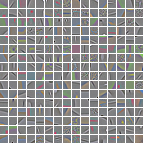
\includegraphics[height=\codeheight\linewidth]{figs/sizematters/centroids/dictionary_ap.png}\qquad\qquad
        
\includegraphics[height=\codeheight\textwidth]{figs/sizematters/centroids/1-neighbors.png}
        
\includegraphics[height=\codeheight\textwidth]{figs/sizematters/centroids/2-neighbors.png}
        
\includegraphics[height=\codeheight\textwidth]{figs/sizematters/centroids/6-neighbors.png}
        
\includegraphics[height=\codeheight\textwidth]{figs/sizematters/centroids/89-neighbors.png}
        
\includegraphics[height=\codeheight\textwidth]{figs/sizematters/centroids/42-neighbors.png}
        
\includegraphics[height=\codeheight\textwidth]{figs/sizematters/centroids/38-neighbors.png}
        
\includegraphics[height=\codeheight\textwidth]{figs/sizematters/centroids/44-neighbors.png}
        
\includegraphics[height=\codeheight\textwidth]{figs/sizematters/centroids/110-neighbors.png}
        
\includegraphics[height=\codeheight\textwidth]{figs/sizematters/centroids/156-neighbors.png}
        
\includegraphics[height=\codeheight\textwidth]{figs/sizematters/centroids/160-neighbors.png}
        
\includegraphics[height=\codeheight\textwidth]{figs/sizematters/centroids/162-neighbors.png}
        
\includegraphics[height=\codeheight\textwidth]{figs/sizematters/centroids/200-neighbors.png}
        
\includegraphics[height=\codeheight\textwidth]{figs/sizematters/centroids/205-neighbors.png}
        
\includegraphics[height=\codeheight\textwidth]{figs/sizematters/centroids/212-neighbors.png}
        
\includegraphics[height=\codeheight\textwidth]{figs/sizematters/centroids/216-neighbors.png}
        
\includegraphics[height=\codeheight\textwidth]{figs/sizematters/centroids/222-neighbors.png}
        
\includegraphics[height=\codeheight\textwidth]{figs/sizematters/centroids/229-neighbors.png}
    \caption{Visualization of the learned codes. Left: the selected subset of 256 centroids from an original set of 3200 codes. Right: The similarity between each centroid and the other codes in its cluster. For each column, the first code is the selected centroid, and the remaining codes are in the same cluster represented by it. Notice that while translational invariance is the most dominant factor, our algorithm does find invariances beyond that (e.g., notice the different colors on the last column). Best viewed in color.}\label{fig:centroidcodes}
\end{figure}

\begin{figure}
    \centering
    \begin{tabular}{ccc}
        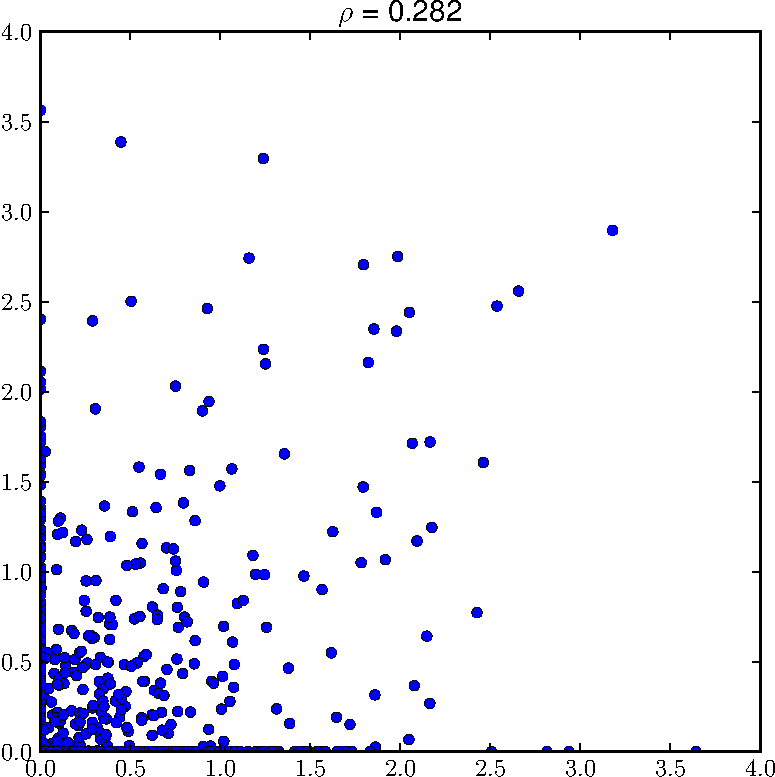
\includegraphics[height=0.25\textwidth]{figs/sizematters/distribution/within_cluster_prepooling.pdf} &
        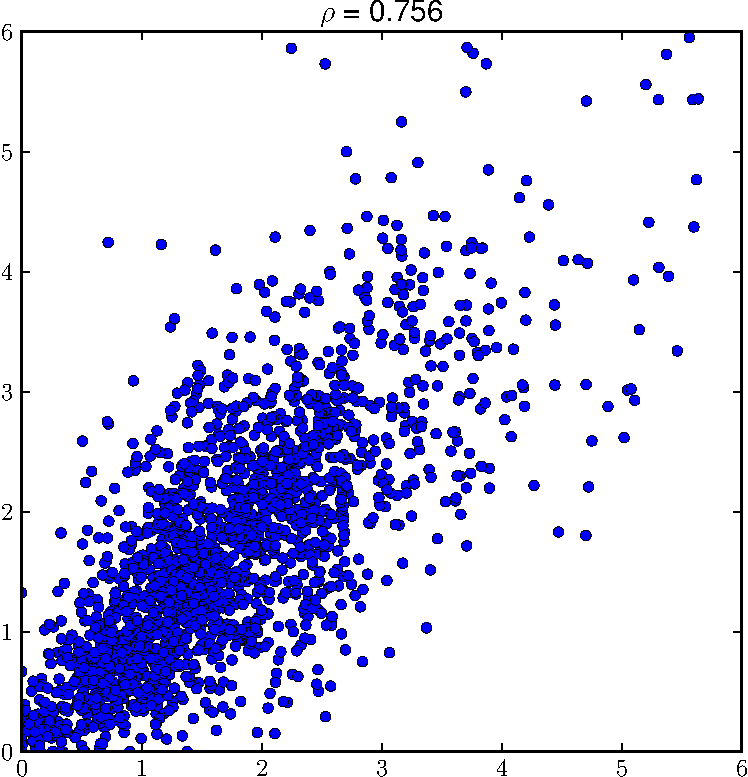
\includegraphics[height=0.25\textwidth]{figs/sizematters/distribution/within_cluster_postpooling.pdf} &
        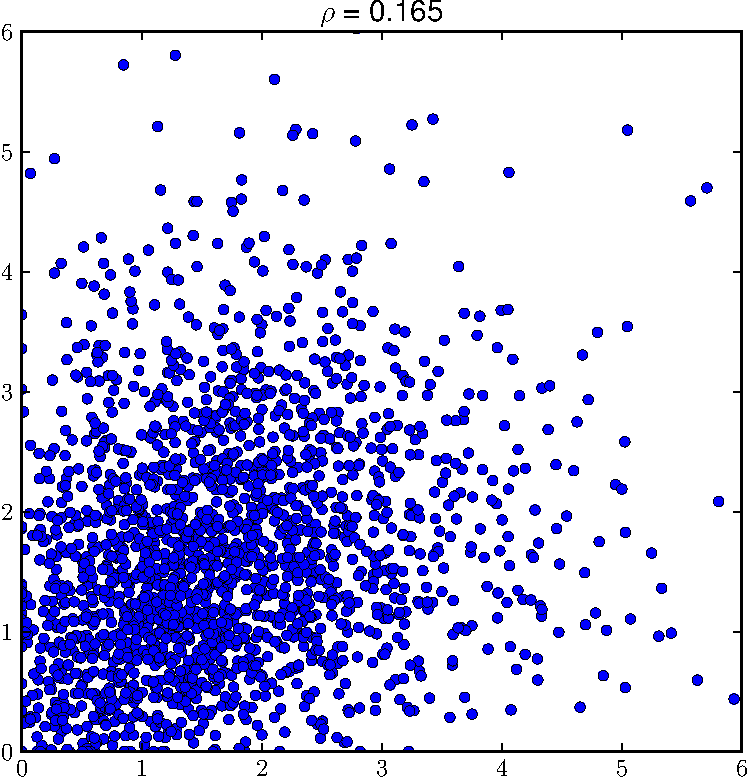
\includegraphics[height=0.25\textwidth]{figs/sizematters/distribution/between_centroids_postpooling.pdf}\\
        (a) & (b) & (c)
    \end{tabular}\\
    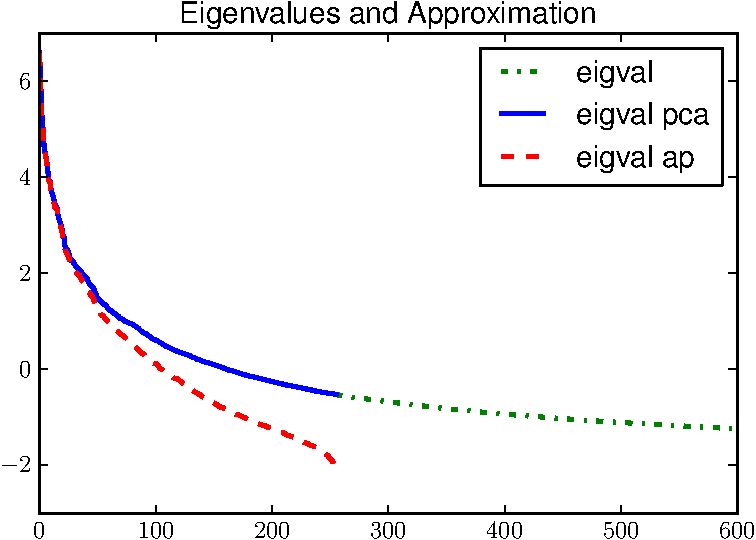
\includegraphics[height=0.3\textwidth]{figs/sizematters/centroids/eigvals.pdf}\\
    (d)
    \caption{(a)-(c): The filter responses before and after pooling: (a) before pooling, between codes in the same cluster (correlation $\rho=0.282$), (b) after pooling, between codes in the same cluster ($\rho = 0.756$), and (c) after pooling, between the selected centroids ($\rho = 0.165$), (d): the eigenvalues of the approximated matrix (in log scale).}\label{fig:pairwiseresponses}
\end{figure}

\subsection{Analysis of Selected Filters}\label{subsec:sizematters:visualization}
To visually show what codes are selected by affinity propagation, we applied our approach to the CIFAR-10 dataset by first training an over-complete dictionary of 3200 codes following \cite{coates2011icml}, and then performing affinity propagation on the 3200-dimensional pooled features to obtain 256 centroids, which we visualize in Figure \ref{fig:centroidcodes}. Translational invariance appears to be the most dominant factor, as many clusters contain translated versions of the same Gabor like code, especially for gray scale codes. On the other hand, clusters capture more than translation: clusters such as column 5 focus on finding the contrasting colors more than finding edges of exactly the same angle, and clusters such as the last column finds invariant edges of varied color. We note that the selected codes are not necessarily centered, as the centroids are selected solely from the pooled response covariance statistics, which does not explicitly favor centered patches.

We could also verify whether the second clustering stage captures the pooling invariance by checking the statistics of three types of filter responses: (a) pairwise filter responses \emph{before pooling} between codes in the same cluster, (b) pairwise filter responses \emph{after pooling} between codes in the same cluster, and (c) pairwise filter responses after pooling between the selected centroids. The distribution of such responses shown in Figure \ref{fig:pairwiseresponses} verifies our argument: first, codes that produce uncorrelated responses before pooling may become correlated after the pooling stage (Figure \ref{fig:pairwiseresponses}(a,b)); second, by explicitly considering the pooled feature statistics, we are able to select a subset of the dictionary whose responses are lowly correlated (Figure \ref{fig:pairwiseresponses}(b,c)), preserving more information with a fixed number of codes. In addition, Figure \ref{fig:pairwiseresponses}(d) shows the eigenvalues of the original covariance matrix and those of the approximated matrix, showing that the approximation captures the largest eigenvalues of the original covariance matrix well.

\begin{table}
    \centering
    \begin{tabular}{ccc}
    \hline
    %\abovespace\belowspace
    Task & Learning Method & Accuracy\\
    \hline
    %\abovespace
                & K-means   & 69.02 \\
    CIFAR-10    & 2x PADL    & 70.54 (+1.52) \\
    200 codes   & 4x PADL    & 71.18 (+2.16) \\
    %\belowspace
                & 8x PADL    & 71.49 (+2.47) \\
    \hline
    %\abovespace
    CIFAR-10    & K-means   & 77.97 \\
    %\belowspace
    1600 codes  & 2x PADL    & 78.71 (+0.74) \\
    \hline
  \end{tabular}
  \caption{Classification Accuracy on the CIFAR-10 and STL datasets under different budgets.}\label{tab:cifarstl}
\end{table}

\begin{figure}[t]
    \centering
    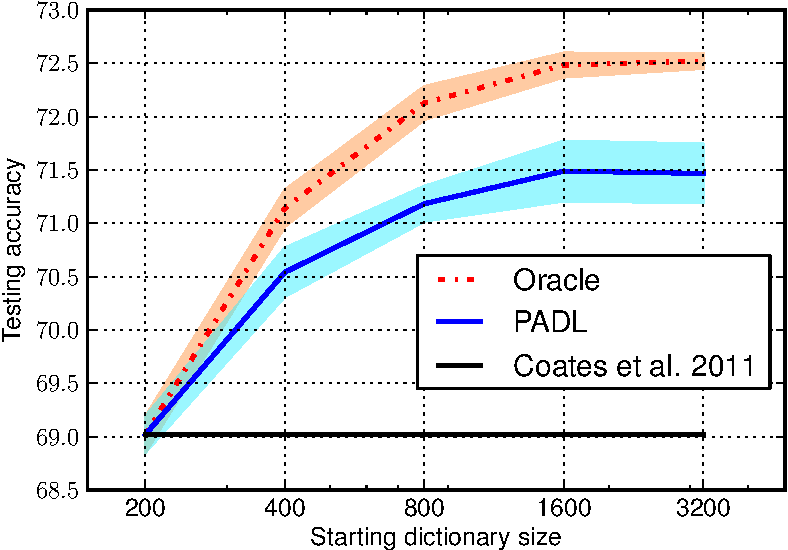
\includegraphics[width=0.5\textwidth]{figs/sizematters/cifar_improvement.pdf}
    \caption{Performance improvement on CIFAR when using different starting dictionary sizes and a final dictionary of size 200. Shaded areas denote the standard deviation over different runs. Note that the x-axis is in log scale.}\label{fig:relativeimprovement}
\end{figure}

\subsection{Pooling Invariant Dictionary Learning}\label{subsec:sizematters:exp:classification}
To evaluate the improvement introduced by learning a pooling invariant dictionary as in Section \ref{sec:sizematters:algorithm}, we show in Figure \ref{fig:relativeimprovement} the relative improvement obtained on CIFAR-10 when we use a fixed dictionary size 200, but perform feature selection from a larger overshooting dictionary as indicated by the X axis. The SVD performance is also included in the figure as an ``oracle'' for the feature selection performance. Learning the dictionary with our feature selection method consistently increases the performance as the size of the original dictionary increases, and is able to get about two thirds the performance gain as obtained by the oracle performance. We note again that SVD still requires the large dictionary to be used and does not save any testing time.

The detailed performance gain of our algorithm on the two datasets, using different overshooting and final dictionary sizes, is visualized in Figure \ref{fig:cifarstl}. Table \ref{tab:cifarstl} summarizes the accuracy values of two particular cases - final dictionary sizes of 200 and 1600 respectively, on CIFAR. Note that our goal is not to get the best overall performance - as performance always goes up when we use more codes. Rather, we focus on two evaluations: (1) how much gain we get given a fixed dictionary size as the budget, and (2) how much computation time we save to achieve the same accuracy.

Overall, considering the pooled feature statistics always help us to find better dictionaries, especially when relatively small dictionaries are used. During testing time, it costs only about 60\% computation time with PADL to achieve the same accuracy as K-means does. For the STL dataset, an overly large starting dictionary may lessen the performance gain (Figure \ref{fig:cifarstl}(b)) possibly due to feature selection being more prone to local optimum and the small number of training data (thus more overfitting). However, in general the codebook learned by PADL is consistently better than its patch-based counterpart, suggesting the applicability of the \nystrom sampling view in feature learning with a multi-layer structure including spatial pooling.

\begin{figure}
    \centering
    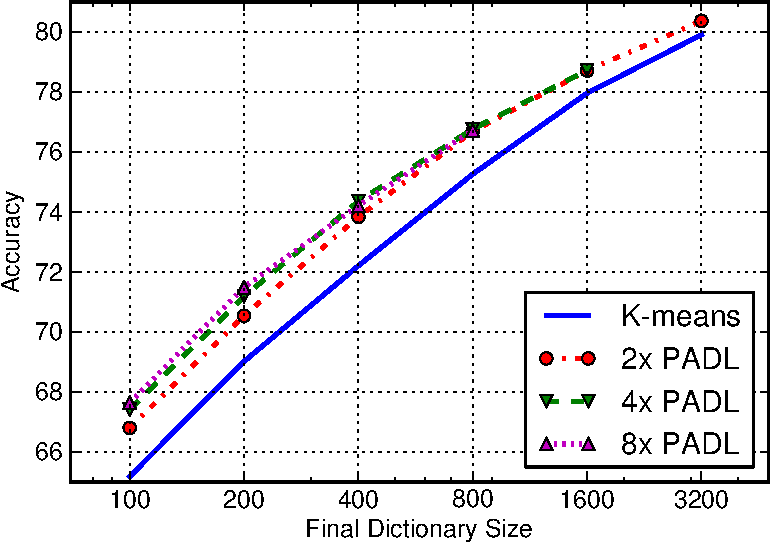
\includegraphics[width=0.4\textwidth]{figs/sizematters/cifar_accuracy.pdf}
    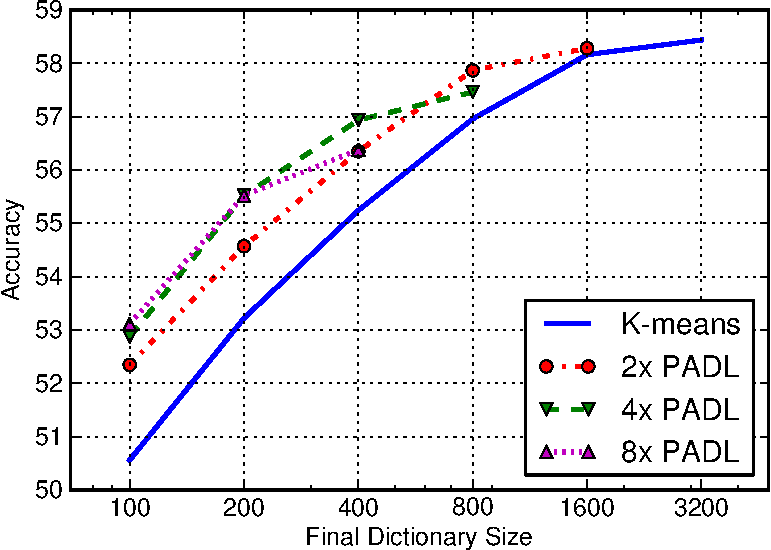
\includegraphics[width=0.4\textwidth]{figs/sizematters/stl_accuracy.pdf}\\
    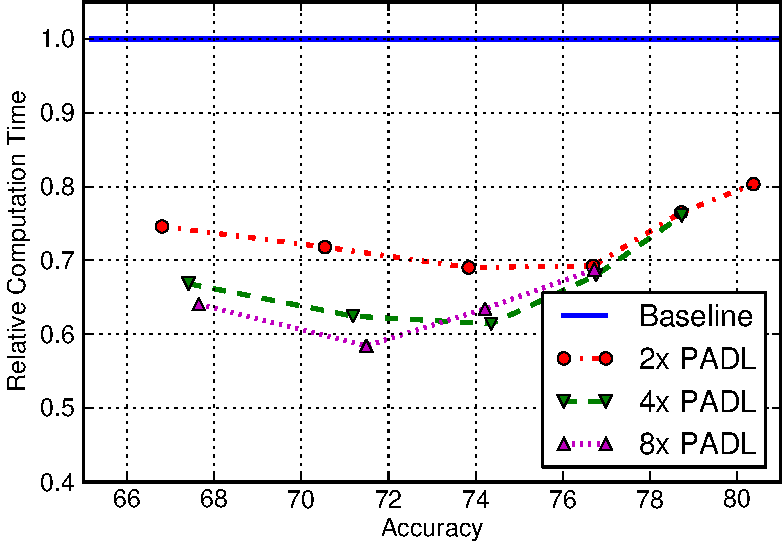
\includegraphics[width=0.4\textwidth]{figs/sizematters/cifar_speedup.pdf}
    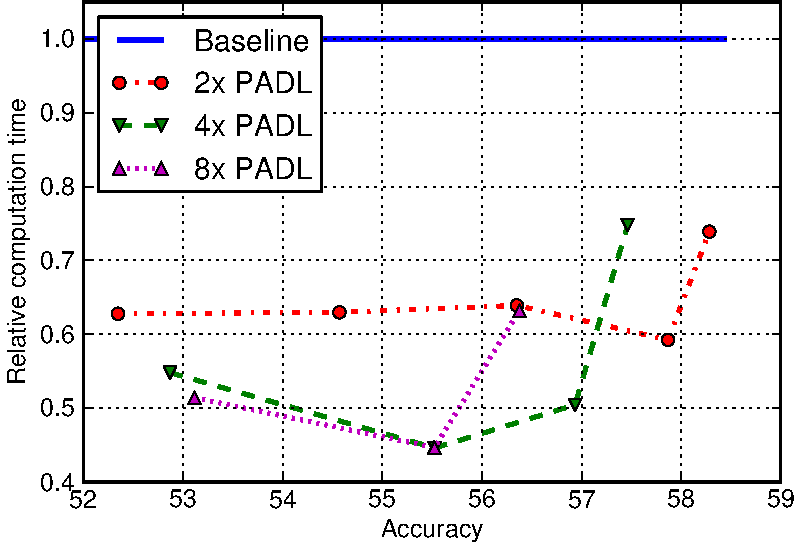
\includegraphics[width=0.4\textwidth]{figs/sizematters/stl_speedup.pdf}
    \caption{Above: accuracy values on the CIFAR-10 (left) and STL (right) datasets under different dictionary size budgets. ``nx PADL'' means learning the dictionary from a starting dictionary that is n times larger. Below: Relative computation time to achieve the same accuracy using dictionary obtained from PADL.}\label{fig:cifarstl}
\end{figure}

Finally, we note that due to the heavy-tailed nature of the encoded and pooled features (see the eigendecomposition of Figure \ref{fig:pairwiseresponses}), one can infer that the representations obtained with a budget would have a correspondingly bounded performance when combined with linear SVMs. We have focused on analyzing unsupervised approaches, but incorporating weakly supervised information to guide feature learning / selection or learning multiple layers of feature extraction would be particularly interesting, and would be a possible future direction.



\chapter{Visual Concept Learning}

Having analyzed the feature generation pipeline for image classification, in this chapter we move on to a higher-level question: how to learn a visual system that infers latent concepts from exemplar images from that concept, a behavior human are known to perform well? To this end, we introduce the cognitive science aspect of the question, and introduce a novel, practical problem that we call \emph{visual concept learning}. We will then bring together findings in cognitive science and computer vision, using machine vision systems to assign novel images locations within a conceptual hierarchy and a Bayesian generalization model to determine how to generalize from these examples.

The result of such effort is a system that comes closer to human performance than state-of-the-art machine vision techniques. Since no existing dataset adequately tests human-like visual concept learning, we have also collected and made available to the community the first large-scale dataset for evaluating whether machine vision algorithms can learn concepts that agree with human perception and label new unseen images, with ground-truth labeling directly obtained from human annotators. We believe that this new task provides challenges beyond the conventional object classification paradigms.

% The visual concept learning part.

\section{The Visual Concept Learning Problem}

We will first formally define visual concept learning, with the protocol developed in earlier cognitive science work such as \cite{xu2007word}. In our task, an agent (either a computer system or a human participant) aims to learn a novel visual concept from a few example images presented to the agent. Such images are randomly sampled from this unknown concept, and no negative examples are provided, similar to how human learn novel words from a few examples\footnote{While one may argue that human receive negative feedbacks as well, such information are often only sought for in an active learning fashion, after the initial concept learning behavior with a few positive examples.}. The agent then has to indicate whether new ``query'' image are or are not instances of the target concept.

A key aspect of this task is determining the degree to which the concept should be generalized \cite{xu2007word} when multiple concepts are logically consistent with the given examples: for example, consider the concepts represented by examples in Figure \ref{fig:conceptfigure} (a-c) respectively, and the task of predicting whether new images (d-e) belong to them or not.  The ground truth from human annotators reveals that the level of generalization varies according to the conceptual diversity, with greater diversity leading to broader generalization. In the examples shown in Figure \ref{fig:conceptfigure}, people might identify the concepts as (a) Dalmatians, (b) all dogs, and (c) all animals, but not generalize beyond these levels although no negative images forbids so.

Bayesian models of generalization \cite{abbott2012, tenenbaum99, xu2007word} account for these phenomena, determining the scope of a novel concept (e.g., does the concept refer to Dalmatians, all dogs, or all animals?) in a similar manner to people. However, these models were developed by cognitive scientists interested in analyzing human cognition, and require examples to be manually labeled as belonging to a particular leaf node in a conceptual hierarchy. This is reasonable if one is asking whether proposed psychological models explain human behavior, but prevents the models from being used to automatically solve visual concept learning problems for a robot or intelligent agent. Machine vision algorithms, on the other hand, still lacks the ability to choose the right level of generalization from the set of valid labels, despite recent successes in large-scale category-level object recognition. We will show in the experiments that state-of-the-art machine vision systems fail to exhibit such patterns of generalization, and have great difficulty learning without negative examples.

\begin{figure}[t]
    \centering
    \newcommand{\demoim}[1]{\includegraphics[height=0.085\linewidth]{figs/vcl/imagenet/#1.png}}
    \begin{tabular}{ccc}
        (a)~\demoim{11437}\demoim{51840}\demoim{89016}\demoim{59577}\demoim{77418} &
        (b)~\demoim{1932}\demoim{11001}\demoim{123075}\demoim{143639}\demoim{81781}\\
        (c)~\demoim{19428}\demoim{126188}\demoim{28487}\demoim{97720}\demoim{112513}&
        (d)~\demoim{maddie} \hspace{0.3in}(e)~\demoim{848}\\
    \end{tabular}
    \caption{Visual concept learning. (a-c): positive examples of three visual concepts. Even without
      negative data, people are able to learn these concepts: (a)
      Dalmatians, (b) dogs and (c) animals. Note that although (a)
      contains valid examples of dogs and both (a) and (b) contain valid
      examples of animals, people restrict the scope of generalization to
      more specific concepts, and find it easy to make judgments about
      whether novel images such as (d) and (e) are instances of the same
      concepts -- the task we refer to as {\em visual concept learning}.}
\end{figure}\label{fig:conceptfigure}

\subsection{Background}

Machine vision methods have achieved considerable success in recent years, as evidenced by performance on major challenge problems \cite{imagenet,pascal}, where strong performance has been obtained for assigning one of a large number of labels to each of a large number of images. However, this research has largely focused on a fairly narrow task: assigning a label (or sometimes multiple labels) to a single image at a time. This task is quite different from that faced by a human child trying to learn a new word, where the child is provided with multiple positive examples and has to generalize appropriately. Even young children are able to learn novel visual concepts from very few positive examples \cite{carey1978}, something that still poses a challenge for machine vision systems.

scant attention has been given to the problem of learning a visual concept from a few positive examples as we have defined it. When the problem has been
addressed, it has largely been considered from a hierarchical regularization
\cite{salakhutdinov2011learning} or transfer learning
\cite{quattoni2008transfer} perspective, assuming that a fixed
set of labels are given and exploiting transfer or regularization within a
hierarchy. Mid-level representations based on attributes
\cite{farhadi2009describing,parikh2011relative} focus on extracting common
attributes such as ``fluffy'' and ``aquatic'' that could be used to
semantically describe object categories better than low-level
features. Transfer learning approaches have been proposed to jointly learn
classifiers with structured regularization \cite{quattoni2008transfer}. Of all these previous efforts, work
that uses object hierarchies to support classification is particularly interesting to our problem scenario. Salakhutdinov et
al.~\cite{salakhutdinov2011learning} proposed learning a set of object
classifiers with regularization using hierarchical knowledge, which
improves the classification of objects at the leaves of the hierarchy.
However, this work did not address the problem of determining the level of
abstraction within the hierarchy at which to make generalizations, which
is a key aspect of the visual concept learning problem. Deng et
al.~\cite{deng2012hedging} proposed predicting object labels only to a
granularity that the classifier is confident with, but their goal
was minimizing structured loss rather than mimicking human generalization.

On the other hand, existing models from cognitive science mainly focus on understanding
human generalization judgments within fairly restricted domains. Tenenbaum
and colleagues \cite{tenenbaum99,tenenbaum2001generalization} proposed
mathematical abstractions for the concept learning problem, building on
previous work on models of generalization by Shepard \cite{shepard87}. Xu
and Tenenbaum~\cite{xu2007word} and Abbott et al.~\cite{abbott2012} conducted
experiments with human participants that provided support for this
Bayesian generalization framework. Xu and Tenenbaum \cite{xu2007word} showed participants one or more positive examples of a novel word (e.g., ``these three objects are Feps''), while manipulating the taxonomic relationship between the examples. For instance, participants could see three toy Dalmatians, three toy dogs, or three toy animals. Participants were then asked to identify the other ``Feps'' among a variety of both taxonomically related and unrelated objects presented as queries. If the positive examples were three Dalmatians, people might be asked whether other Dalmatians, dogs, and animals are Feps, along with other objects such as vegetables and vehicles. Subsequent work has used the same basic methodology in experiments using a manually collated set of images as stimuli \cite{abbott2012}. All of these models assume that objects
are already mapped onto locations in a perceptual space or conceptual
hierarchy. Thus, they are not able to make predictions about genuinely
novel stimuli. Linking such generalization models to direct perceptual
input is necessary in order to be able to use this approach to learn
visual concepts directly from images.




\section{A Large-scale Concept Learning Dataset}\label{sec:mechturk}

Existing datasets (PASCAL \cite{pascal}, ILSVRC \cite{ilsvrc}, etc.) test supervised learning performance with relatively large amounts of positive and negative examples available, with ground truth as a set of mutually-exclusive labels. To our knowledge, no existing dataset accurately captures the task we refer to as visual concept learning: to learn a novel word from a small set of positive examples like humans do. In this section, we describe in detail our effort to make available a dataset for such task.

\subsection{Test Procedure}

In our test procedure, an agent is shown $n$ example images ($n=5$ in our dataset) sampled from a node (may be leaf nodes or intermediate nodes) from the ImageNet synset tree, and is then asked whether other new images sampled from ImageNet belong to the concept or not. The scores that the agent gives are then compared against human ground truth that we collect, and we use precision-recall curves to evaluate the performance.

We use the ImageNet ILSVRC 2010 synset tree as the beginning point of our data generation procedure for several reasons. First, the ImageNet synset tree is derived from WordNet, which well models the semantics between synsets in a nicely hierarchical structure. Second, ImageNet comes with a large number of image collections manually verified by human whether they belong to the correct synset or not, providing us a large-scale pool for test images. Third, the large number of images allows one to train visual classifiers\footnote{This is analogy to the development of the visual system from a vast number of perceptual input during infant years.} that identifies images into one of the basic concepts (leaf nodes in the tree), serving as a perceptual basis for concept learning.

From a machine vision perspective, one may ask whether this visual concept learning task differs from the conventional ImageNet-defined classification problem -- identifying the node from which the examples are drawn, and then answering yes for images in the subtree corresponding to the node, and no for images not from the node. We note that, although we use the nodes in the ImageNet tree to generate examples and queries, the tree itself may not be an accurate hierarchy that matches human perception, and should only be treated as a proxy instead of ground truth. Thus, actual human behavior may differ from what the tree structure implies,In fact, we will show in Section 5.2 that using this approach fails to explain how people learn visual concepts. Human performance in the above task exhibits much more sophisticated concept learning behaviors than simply identifying the node itself, and the latter differs significantly from what we observe from human participants. In addition, with no negative images, a conventional classification model fails to distinguish between nodes that are both valid candidates (\eg ``dogs'' and ``animals'' when shown a bunch of dog images). These make our visual concept learning essentially different and richer than a conventional classification problem.

\subsection{Automatic Generation of Examples and Queries}

Large-scale experimentation requires an efficient scheme to generate test data across varying levels of a concept hierarchy. To this end, we developed a fully-automated procedure for constructing a large-scale dataset suitable for a challenge problem focused on visual concept learning. We used the ImageNet LSVRC \cite{ilsvrc} 2010 data as the basis for automatically constructing a hierarchically-organized set of concepts at four different levels of abstraction. We had two goals in constructing the dataset: to cover concepts at various levels of abstraction (from subordinate concepts to superordinate concepts, such as from “Dalmatian” to “living things”), and to find query images that comprehensively test human generalization behavior. We address these two goals in turn.

To generate concepts at various levels of abstraction, we use all the nodes in the ImageNet hierarchy as concept candidates, starting from the leaf node classes as the most specific level concept. We then generate three more levels of increasingly broad concepts along the path from the leaf to the root for each leaf node in the hierarchy. Examples from such concepts are then shown to human participants to obtain human generalization judgements, which will serve as the ground truth. Specifically, we use the leaf node class itself as the most basic trial type $L_0$, and select three levels of nested concepts $L_1$, $L_2$, $L_3$ which correspond to three intermediate nodes along the path from the leaf node to the root. We choose the three nodes that maximize the combined information gain across these levels:
\begin{equation}
    \mathcal{C}(L_{1\cdots 3}) = \sum\nolimits_{i=0}^{3} \log(|L_{i+1}| - |L_{i}|) - \log|L_{i+1}|,
\end{equation}
where $|L_i|$ is the number of leaf nodes under the subtree rooted at $L_i$, and $L_4$ is the whole taxonomy tree. As a result, we obtain levels that are ``evenly'' distributed over the taxonomy tree. Such levels coarsely correspond to the sub-category, basic, super-basic, and super-category levels in the taxonomy: for example, the four levels used in Figure \ref{fig:conceptfigure} are {\texttt dalmatian}, {\texttt domestic dog}, {\texttt animal}, {\texttt organism} for the leaf node {\texttt dalmatian}, and in Figure \ref{fig:trials}(a) are {\texttt blueberry}, {\texttt berry}, {\texttt edible fruit}, and {\texttt natural object} for the leaf node {\texttt blueberry}. Figure \ref{fig:trials}(b) shows a histogram of the subtree sizes for $L_1$ to $L_3$ respectively.

%For each concept, we then randomly sample five images from five different leaf node categories from the corresponding subtree%\footnote{If there are $<5$ leaves, each leaf is selected once and the remaining counts sampled with replacement.}
%from the ILSVRC 2010 test images as examples shown to the participants about the concept.
For each concept, the five images shown to participants as examples of that concept were randomly sampled from five different leaf node categories from the corresponding subtree in the ILSVRC 2010 test images. Figure \ref{fig:conceptfigure} and \ref{fig:trials} show such examples.
%We note that the ImageNet nodes are used as a proxy to generate examples, and may be different from the ground truth for concept learning, which we will collect from human experiments.

To obtain the ground truth (the concepts people perceive when given the set of examples), we then randomly sample twenty query images, and ask human participants whether each of these query images belong to the concept given by the example images. A total of 20 images are randomly sampled as follows: three each from the $L_0$, $L_1$, $L_2$ and $L_3$ subtrees, and eight images outside $L_3$. This ensures a complete coverage over in-concept and out-of-concept queries. We explicitly made sure that the leaf node classes of the query images were different from those of the examples if possible, and no duplicates exist among the 20 queries. Note that we always sampled the example and query images from the ILSVRC 2010 test images, allowing us to subsequently train our machine vision models with the training and validation images from the ILSVRC dataset while keeping those in the visual concept learning dataset as novel test images.

\begin{figure}
  \newcommand{\berryim}[1]{\includegraphics[width=0.09\textwidth]{figs/vcl/imagenet/#1.png}}
  \newcommand{\queryim}[1]{\includegraphics[width=0.09\textwidth]{figs/vcl/imagenet/#1.png}}
  \begin{center}
  \begin{tabular}{cc}
  \berryim{7108}\berryim{124489}\berryim{20860}\berryim{16423}\berryim{21453} &
  \berryim{8468}\berryim{89717}\berryim{26147}\berryim{58871}\berryim{80140} \\
  blueberry & berry \\
  \berryim{16325}\berryim{69947}\berryim{39119}\berryim{58034}\berryim{46119} &
  \berryim{121321}\berryim{95236}\berryim{114712}\berryim{44258}\berryim{112827}\\
  edible fruit & natural object
  \end{tabular}
  \end{center}

  \begin{center}
  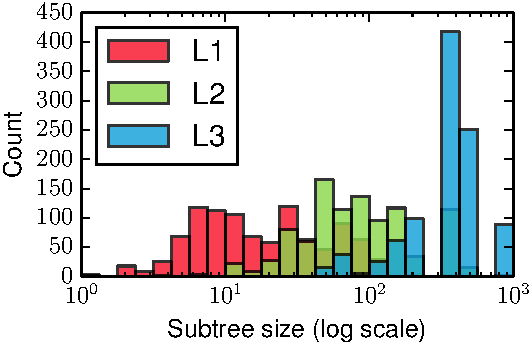
\includegraphics[width=0.5\textwidth]{figs/vcl/trialtype_histogram.pdf}
  \end{center}
  \caption{Concepts drawn from ImageNet.Top: example images sampled from the four levels for {\texttt blueberry}. Bottom: the histogram for the subtree sizes of different levels of concepts (x axis in log scale).}
  \label{fig:trials}
\end{figure}

\subsection{Collecting Human Judgements}

We created 4,000 identical concepts (four for each leaf node) using the protocol above, and recruited participants online through Amazon Mechanical Turk (AMT, \url{http://www.mturk.com}) to obtain the human ground truth data. For each concept, an AMT HIT (a single task presented to the human participants) is formed with five example images and twenty query images. The participants were presented with a display where they could easily click what query images belong to the given
category or not. Following previous work, participants were told that ``Mr. Frog'' had picked
out some examples of a word in a different language (using a randomly generated word that beared no actual meaning in order to minimize influence from languages), and that ``Mr. Frog'' needed help picking out the other objects that could be called that word (see Figure 1 for the precise wording). Figure \ref{fig:mrfrog} shows an example display that a participant could have seen, and possible response from a participant for this trial (all buttons were initialized grey before the participant clicks).

\begin{figure}
  \centering
  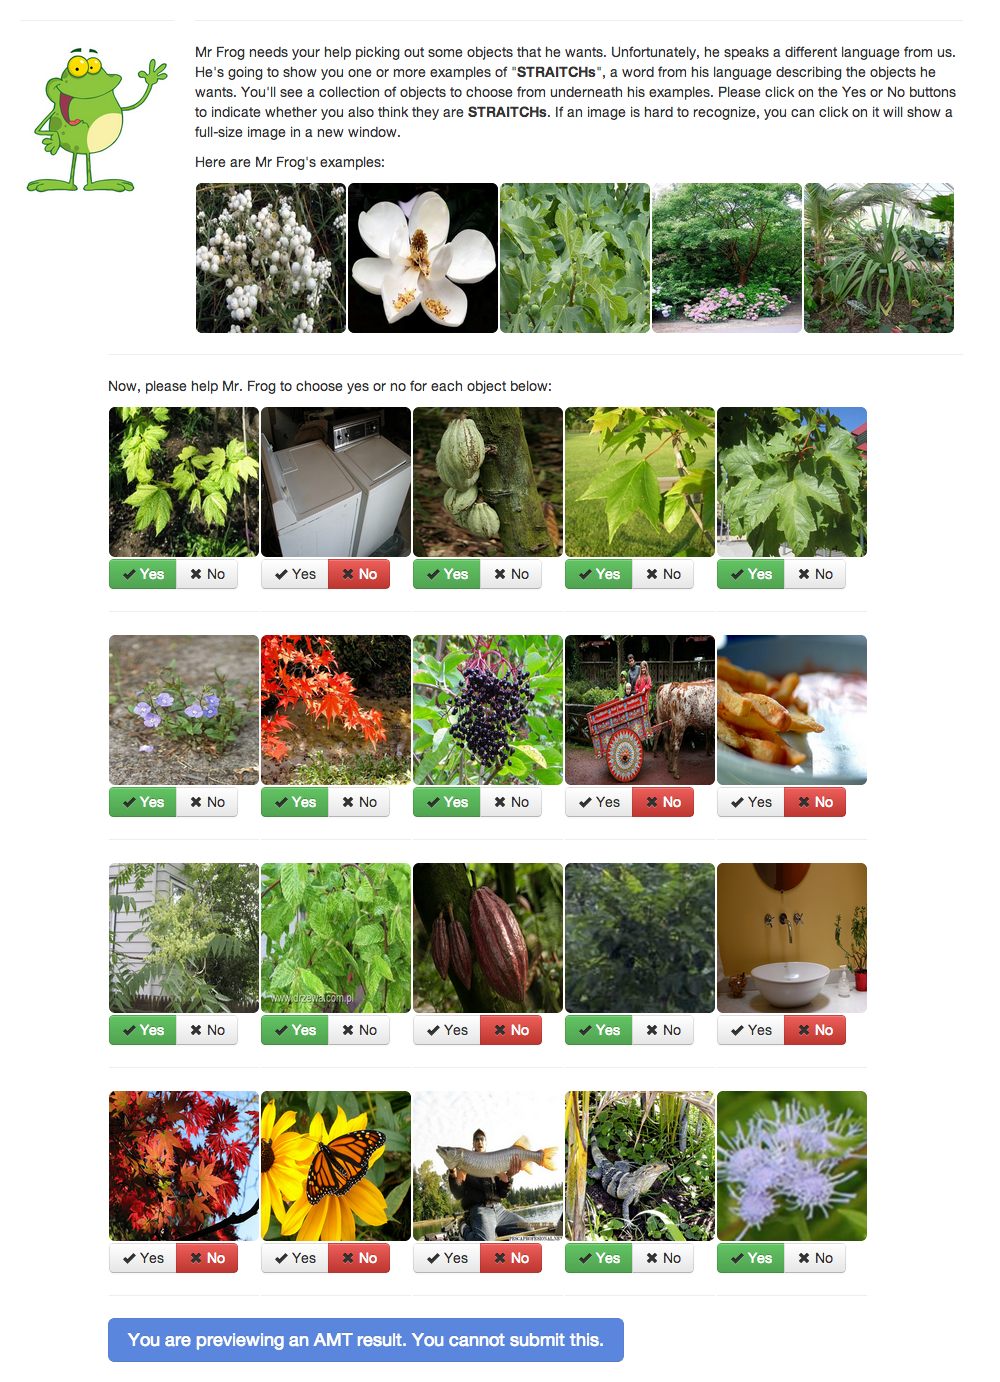
\includegraphics[width=0.9\textwidth]{figs/vcl/amt/amt_page_with_result.png}
  \caption{An example display that we used for the Mechanical Turk interface, together with the response from the participant.}\label{fig:mrfrog}
\end{figure}

Each HIT was completed by five unique participants, with a compensation of \$0.05 USD per HIT. Participants were allowed to complete as many unique trials as they wished. Thus, a total of 20,000 AMT HITs were collected, and a total of 100,000 images were shown to the participants. On average, each participant took approximately one minute to finish each HIT, spending about 3 seconds per query image.


\section{Visually-Grounded Bayesian Concept Learning}

In this section, we describe an end-to-end framework which combines Bayesian word learning models and visual classifiers, and is able to perform concept learning with perceptual inputs. 

\subsection{Bayesian Concept Learning}
Prior work on concept learning \cite{xu2007word} addressed the problem of generalization from examples using a Bayesian framework: given a set of $N$ examples (images in our case) $\mathcal{X} = \{ \bx_1, \bx_2,\ldots, \bx_N \}$ that are members of an unknown concept $\mathcal{C}$, the probability that a query instance $\bx_\mathrm{query}$ also belongs to the same concept is given by
\begin{equation}
P_{\mathrm{new}}(\bx_\mathrm{query} \in \mathcal{C}|\mathcal{X}) = \sum\nolimits_{h \in \mathcal{H}} P_{\mathrm{new}}(\bx_\mathrm{new} | h)P(h|\mathcal{X}), \label{eq:bayeswl}
\end{equation}
where $\mathcal{H}$ is called the ``hypothesis space'' -- a set of possible hypotheses for what the concept might be. Each hypothesis corresponds to a (often semantically related) subset of all the objects in the world, such as ``dogs'' or ``animals''. Given a specific hypothesis $h$, the probability $P_{\mathrm{new}}(x_\mathrm{new}|h)$ that a new instance belongs to it is $1$ if $x_\mathrm{new}$ is in the set, and $0$ otherwise, and $P(h | \mathcal{X})$ is the \emph{posterior} probability of a hypothesis $h$ given the examples $\mathcal{X}$.
%We assume the objects form a taxonomic hierarchy, where each object $x_n$ belongs to one leaf node in a rooted tree and hypotheses $h_k$ are internal nodes such that $x_n \in h_k$ if $x_n$ is a descendant of $h_k$.

The posterior distribution over hypotheses is computed using the Bayes' rule: it is proportional to the product of the {\em likelihood}, $P(\mathcal{X} | h)$, which is the probability of drawing these examples from the hypothesis $h$ uniformly at random times the {\em prior} probability $P(h)$ of the hypothesis:
\begin{equation}
    P(h|\mathcal{X}) \propto P(h)\prod\nolimits_{i=1}^{N}P_{\mathrm{example}}(\bx_i | h),
\end{equation}
where we also make the strong sampling assumption that each $\bx_i$ is drawn uniformly at random from the set of instances picked out by $h$. Importantly, this ensures that the model acts in accordance with the ``size principle'' \cite{tenenbaum99,tenenbaum2001generalization}, meaning that the conditional probability of an instance given a hypothesis is inversely proportional to the size of the hypothesis, \ie the number of possible instances that could be drawn from the hypothesis:
\begin{equation}
    P_{\mathrm{example}}(\bx_i | h) = |h|^{-1}I(\bx_i \in h),
\end{equation}
where $|h|$ is the size of the hypothesis and $I(\cdot)$ is an indicator function that has value 1 when the statement is true. We note that the probability of an \emph{example} and that of a \emph{query} given a hypothesis are different: the former depends on the size of the underlying hypothesis, representing the nature of training with strong sampling. For example, as the number of examples that are all Dalmatians increases, it becomes increasingly likely that the concept is just Dalmatians and not dogs in general even though both are logically possible, because it would have been incredibly unlikely to only sample Dalmatians given that the truth concept was dogs. In addition, the prior distribution $P(h)$ captures biases due to prior knowledge, which favor particular kinds of hypotheses over others (which we will discuss in the next subsection). For example, it is known that people favor basic level object categories such as dogs over subcategories (such as Dalmatians) or supercategories (such as animals).

\subsection{Concept Learning with Perceptual Uncertainty}
Existing Bayesian word learning models assume that objects are perfectly recognized, thus representing them as discrete indices into a set of finite tokens. Hypotheses are then subsets of the complete set of tokens and are often hierarchically nested. Although perceptual spaces were adopted in \cite{tenenbaum99}, only very simple hypotheses (rectangles over the position of dots) were used. Performing Bayesian inference with a complex perceptual input such as images is thus still a challenge. To this end, we utilize the state-of-the-art image classifiers and classify each image into the set of leaf node classes given in the ImageNet hierarchy, and then build a hypothesis space on top of the classifier outputs.
%In other words, the classifier outputs could be seen as sufficient statistics of the images.

Specifically, we construct the hypothesis space over the image labels using the ImageNet hierarchy, with each subtree rooted at a node serving as a possible hypothesis. The hypothesis sizes are then computed as the number of leaf node classes under the corresponding node, \eg the node ``animal'' would have a larger size than the node ``dogs''. The large number of images collected by ImageNet allows us to train classifiers from images to the leaf node labels, which we will describe shortly. Assuming that there are a total of $K$ leaf nodes, for an image $\bx_i$ that is classified as label $\hat{y}_i$, the likelihood $P(\bx_i | h)$ is then defined as
\begin{equation}
    P_{\mathrm{example}}(\bx_i | h) = \sum\nolimits_{j=1}^{K}A_{j\hat{y}_i}\frac{1}{|h|}I(j \in h),
\end{equation}
where $\bA$ is the normalized confusion matrix, with $A_{j,i}$ being the probability that the true leaf node is $j$ given the classifier output being $i$. The motivation of using the confusion matrix is that classifiers are not perfect and misclassification could happen. Thus, the use of the confusion matrix incorporates the visual ambiguity into the word learning framework by providing an unbiased estimation of the true leaf node label for an image.
%\footnote{Another option is to use the confidence score by the classifiers as a probability measure. We experimented with both and found the confusion matrix approach to be empirically better.}.

The prior probability of a hypothesis was defined to be an Erlang distribution, $P(h)\propto (|h|/\sigma^2)\exp\{-|h|/\sigma\}$, which is a standard prior over sizes in Bayesian models of generalization \cite{shepard87, tenenbaum2000rules}. The parameter $\sigma$ is set to 200 according to \cite{abbott2012} in order to fit human cognition, which favors basic level hypotheses \cite{rosch1976basic}. Finally, the probability of a new instance belonging to a hypothesis is similar to the likelihood, but without the size term, as $P_{\mathrm{new}}(\bx_\mathrm{new} | h) = \sum_{j=1}^{K}A_{j\hat{y}_\mathrm{new}}I(\hat{y}_\mathrm{new} \in h)$, where $\hat{y}_\mathrm{new}$ is the classifier prediction.


%To overcome this issue, we train modern image classification techniques to predict the appropriate leaf node (most specific) for an image using the ImageNet database \cite{imagenet}. The output of our classifier is vector whose elements are (noisy) estimations that the image should be labelled by each leaf node. We first discuss training the image classifiers, and then incorporate the output of the classifiers into the Bayesian word learning model.

%ImageNet is a large ontology of images organized in a structure conforming to the WordNet hierarchy, with the aim of providing over 500 high-quality images per noun in WordNet. Abbott et al.\ \cite{abbott2012} proposed that ImageNet could be used to automatically construct stimuli for human experiments, but their model did not assume a vision component and in turn they manually selected stimulus images for each word. On the contrary, we propose to use these images as an input source to train image classifiers. This is the key difference from existing word learning research, as the image classifiers enable us to infer the conceptual labels for new image input.

\subsection{Learning the Perceptual Classifiers}
To train the image classifiers for the perceptual component in our model, we used the ILSVRC training images, which consisted of 1.2 million images categorized into the 1,000 leaf node classes, and followed the pipeline in \cite{lin2011large} to obtain feature vectors to represent the images. This pipeline uses $160$K dimensional features, yielding a total of about $1.5$TB for the training data. 
We trained the classifiers with linear multinomial logistic regressors with minibatch Adagrad \cite{duchi2010adaptive} algorithm, which is a quasi-Newton stochastic gradient descent approach. The hyperparameters of the classifiers are learned with the held-out validation data.

Overall, we obtained a performance of 41.33\% top-1 accuracy and a 61.91\% top-5 accuracy on the validation data, and 41.28\% and 61.69\% respectively on the testing data, and the training took about 24 hours with 10 commodity computers. Although this is not the best ImageNet classifier to date, we believe that the above pipeline is a fair representation of the state-of-the-art computer vision approaches. Algorithms using similar approaches have reported competitive performance in image classification on a large number of classes (on the scale of tens of thousands) \cite{le2012icml, krizhevsky2012imagenet}, which provides reassurance about the possibility of using state-of-the-art classification models in visual concept learning.

To obtain the confusion matrix $\bA$ of the classifiers, we note that the validation data alone does not suffice to provide a dense estimation of the full confusion matrix, because there is a large number of entries (1 million) but very few validation images (50K). Thus, instead of using the validation data for estimation of $\bA$, we approximated the classifier's leave-one-out (LOO) behavior on the training data with a simple one-step gradient descent update to ``unlearn'' each image. Specifically, we started from the trained classifier parameters, and for each training image $\bx$, we compute the gradient of the loss function when $\bx$ is left out of the training set. We then take one step update in the direction of the gradient to obtain the updated classifier, and use it to perform prediction on $\bx$. This allows us to obtain a much denser estimation that worked better than existing methods. We refer the reader to the supplementary material for the technical details about the classifier training and the LOO confusion matrix estimation.


\section{Experiments}
In this section, we describe the experimental protocol adopted to compare our system with human
performance and compare our system against various baseline algorithms.
Quantitatively, we use the precision-recall curve, the average precision (AP) and the $F_1$ score at the point where precision = recall 
%\footnote{Empirically (as shown in Figure \ref{fig:prcurve}), the human participants exhibit approximately the same precision and recall values, so we choose the point on the PR curve where $p = r$, and compute the corresponding $F_1$ score.}
to evaluate the performance and to compare against the human performance, which is calculated by randomly sampling one human participant per distinctive HIT, and comparing his/her prediction against the four others.

To the best of our knowledge, there are no existing vision models that explicitly handles our concept learning task. Thus, we compare our vision baseg Bayes generalization algorithm (denoted by {\bfseries VG}) described in the previous section against the following baselines, which are reasonable extensions of existing vision or cognitive science models:
\begin{enumerate}\setlength{\itemsep}{0pt}\setlength{\parskip}{0pt}
    \item {\bfseries Naive vision approach} (NV): this uses a nearest neighbor approach by computing the score of a query as its distance to the closest example image, using GIST features \cite{oliva2001modeling}.
    \item {\bfseries Prototype model} (PM): an extension of the image classifiers. We use the $L_1$ normalized classifier output from the multinomial logistic regressors as a vector for the query image, and compute the score as its $\chi^2$ distance to the closest example image.
    \item {\bfseries Histogram of classifier outputs} (HC): similar to the prototype model, but instead of computing the distance between the query and each example, we compute the score as the $\chi^2$ distance to the histogram of classifier outputs, aggregated over the examples.
    \item {\bfseries Hedging the bets extension} (HB): we extend the hedging idea \cite{deng2012hedging} to handle sets of query images. Specifically, we find the subtree in the hierarchy that maximizes the information gain while maintaining an overall accuracy above a threshold $\epsilon$ over the set of example images. The score of a query image is then computed as the probability that it belongs to this subtree. The threshold $\epsilon$ is tuned on a randomly selected subset of the data.
    \item {\bfseries Non-perceptual word learning} (NP): the classical Bayesian word learning model in \cite{xu2007word} assuming a perfect classifier, \ie by taking the ground-truth leaf labels for the test images. This is not practical in actual applications, but evaluating NP helps understand how a perceptual component contributes to modeling human behavior.
\end{enumerate}

\begin{figure}
    \centering
    \parbox{0.35\textwidth}{
    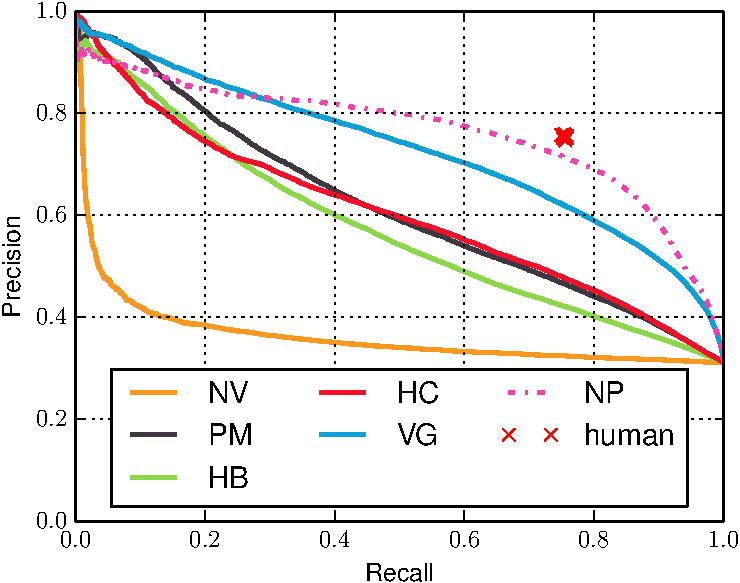
\includegraphics[width=1\linewidth]{figs/vcl/pr_curve.pdf}}\hspace{0.05\textwidth}%
    \parbox{0.4\textwidth}{
        \small
        \begin{tabular}{c|cc}
            \hline\hline
            Method & AP & $F_1$ Score \\
            \hline
            NV & 36.37 & 35.64 \\
            PM & 61.74 & 56.07 \\
            HC & 60.58 & 56.82 \\
            HB & 57.50 & 52.72 \\
            NP & 76.24 & 72.70 \\
            {\bfseries VG (ours)} & 72.82 & 66.97 \\
            \hline
            Human Performance & - & 75.47 \\
            \hline
        \end{tabular}
    }
    \caption{The precision-recall curves of our method and the baseline algorithms. The human results are shown as the red crosses, and the non-perceptual Bayesian word learning model (NB) is shown as magenta dashed lines. The table summarizes the average precision (AP) and $F_1$ scores of the methods.}\label{fig:prcurve}
\end{figure}

\subsection{Main Results}
Figure \ref{fig:prcurve} shows the precision-recall curves for our method and the baseline methods, and summarizes the average precision and $F_1$ scores. Conventional vision approaches that build upon image classifiers work better than simple image features (such as GIST), which is sensible given that object categories provide relatively more semantics than simple features. However, all the baselines still have performances far from human's, because they miss the key mechanism for inferring the ``width'' of the latent concept represented by a set of images (instead of a single image as conventional approaches assume). In contrast, adopting the size principle and the Bayesian generalization framework allows us to perform much better, obtaining an increase of about 10\% in average precision and $F_1$ scores, closer to the human performance than other visual baselines.

The non-perceptual (NP) model exhibits better overall average precision than our method, which suggests that image classifiers can still be improved. This is indeed the case, as state-of-the-art recognition algorithms may still significantly underperform human. However, note that for a system to work in a real-world scenario such as aid-giving robots, it is crucial that the agent be able to take direct perceptual inputs. It is also interesting to note that all visual models yield higher precision values in the low-recall region (top left of Figure \ref{fig:prcurve}) than the NP model, which does not use perceptual input and has a lower starting precision. This suggests that perceptual signals do play an important role in human generalization behaviors, and should not be left out of the pipeline as previous Bayesian word learning methods do.

\begin{figure}[t]
    \centering
    \begin{tabular}{cc}
        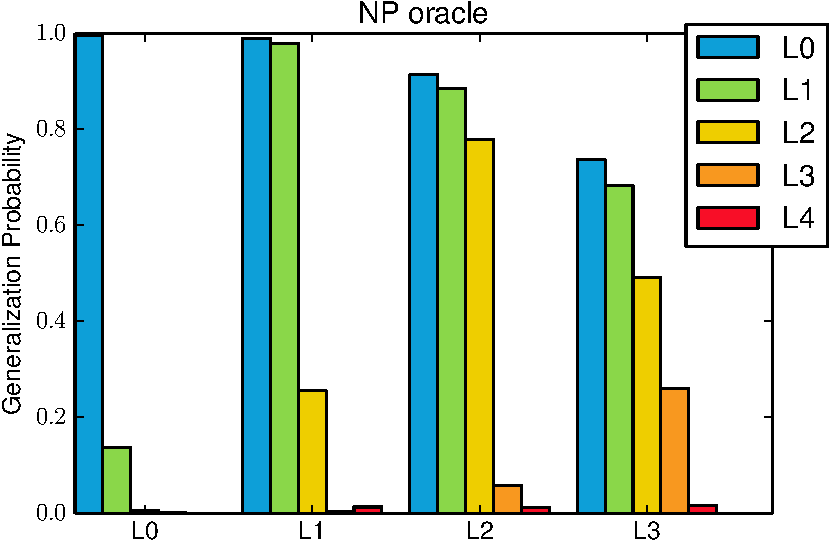
\includegraphics[width=0.28\textwidth]{figs/vcl/per_level_response_np.pdf}
        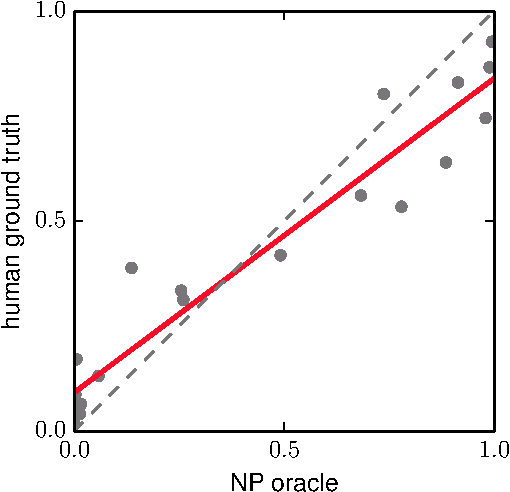
\includegraphics[width=0.15\textwidth]{figs/vcl/correlation_np.pdf} &
        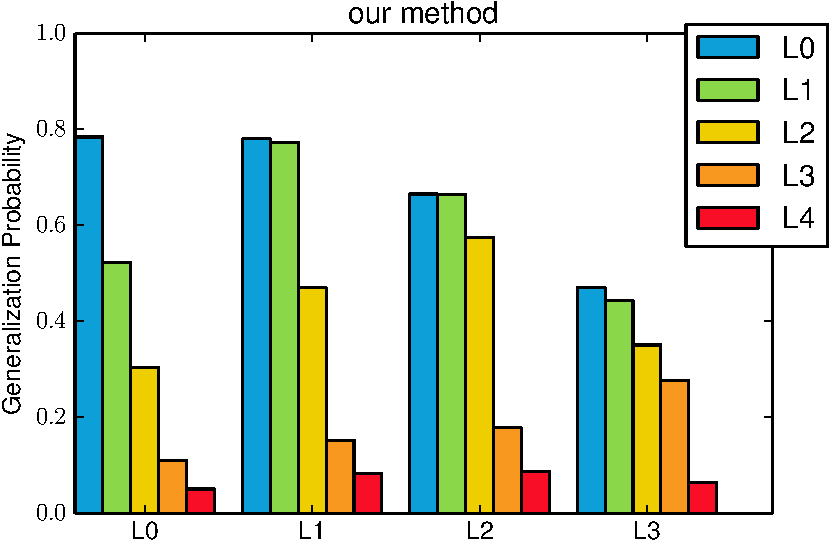
\includegraphics[width=0.28\textwidth]{figs/vcl/per_level_response_vg.pdf}
        \includegraphics[width=0.15\textwidth]{figs/vcl/correlation_vg.pdf}\\
        (a) NP model & (b) Our method \\
        \includegraphics[width=0.28\textwidth]{figs/vcl/per_level_response_pm.pdf}
        \includegraphics[width=0.15\textwidth]{figs/vcl/correlation_pm.pdf} &
        \includegraphics[width=0.28\textwidth]{figs/vcl/per_level_response_ic.pdf}
        \includegraphics[width=0.15\textwidth]{figs/vcl/correlation_ic.pdf}\\
        (c) PM baseline & (d) IC oracle \\
    \end{tabular}
\caption{Per-level generalization predictions from various methods, where the horizontal axis shows four levels at which examples were provided ($L_0$ to $L_3$). At each level, five bars show the proportion of queries form levels $L_0$ to $L_4$ that are labeled as instances of the concept by each method. These results are summarized in a scatter plot showing model predictions (horizontal axis) vs. human judgments (vertical axis), with the red line showing a linear regression fit.}\label{fig:bars}
\end{figure}

\subsection{Analysis of Per-level Responses}\label{subsec:bars}

In addition to the quantitative precision-recall curves, we perform a qualitative per-level analysis similar to previous word learning work \cite{abbott2012}. To this end, we binarize the predictions at the threshold that yields the same precision and recall, and then plot the per-level responses, \ie the proportion of query images from level $L_i$ that are predicted positive, given examples from level $L_j$.

\begin{wrapfigure}{r}{0.4\textwidth}
    \centering
    \includegraphics[width=0.9\linewidth]{figs/vcl/per_level_response_human.pdf}
    \caption{Per-level generalization from human participants.}\label{fig:humanbars}
    %The X-axis shows four groups of example types, from levels $L_0$ to $L_3$ respectively. Within each group, the five bars shows the proportion of queries from levels $L_0$ to $L_4$ that are labeled positive.}
\end{wrapfigure}

We show in Figures \ref{fig:bars} and \ref{fig:humanbars} the per-level generalization results from human, the NP model, our method, and the PM baseline which best represents state-of-the-art vision baselines. People show a monotonic decrease in generalization as the query level moves conceptually further from the examples. In addition, for queries of the same level, its generalization score peaks when examples from the same level are presented, and drops when lower or higher level examples are presented. The NP model tends to give more extreme predictions (either very low or very high), possibly due to the fact that it assumes perfect recognition, while visual inputs are actually difficult to precisely classify even for a human being. The conventional vision baseline does not utilize the size principle to model human concept learning, and as a result shows very similar behavior with different level of examples. Our method exhibits a good correlation with the human results, although it has a smaller generalization probability for $L_0$ queries, possibly because current visual models are still not completely accurate in identifying leaf node classes \cite{deng2012hedging}.

Last but not least, we examine how well a conventional image classification approach could explain our experimental results. To do so, Figure 4\ref{fig:bars}(d) plots the results of an image classification (IC) oracle that predicts yes for an image within the ground-truth ImageNet node that the current examples were sampled from and no otherwise. Note that the IC oracle never generalizes beyond the level from which the examples are drawn, and thus, exhibits very different generalization results compared to the human participants in our experiment. Thus, visual concept learning poses more realistic and challenging problems for computer vision studies.


\section{Conclusions}

We proposed a new task for machine vision -- visual
concept learning -- and presented the first system capable of approaching
human performance on this problem. By linking research on object
classification in machine vision and Bayesian generalization in cognitive
science, we were able to define a system that could infer the appropriate
scope of generalization for a novel concept directly from a set of
images. This system outperforms baselines that draw on previous approaches
in both machine vision and cognitive science, coming closer to human
performance than any of these approaches. However, there is still
significant room to improve performance on this task, and we present our
visual concept learning dataset as the basis for a new challenge problem
for machine vision, going beyond assigning labels to individual objects.

%
%model that accounts for perceptual uncertainty, our approach addresses
%limitations in the existing word learning and image classification
%algorithms: the former only being able to use a limited number of stimuli,
%and the latter not being able to infer the level of generalization. We
%believe that our work is the first to present a model that learns a visual
%concept from sets of raw image input, and to empirically show the
%resemblance of human generalization behavior on a large scale. We hope
%that this work provides common ground for computer vision and cognitive
%science researchers that provides a step towards developing novel object
%recognition algorithms that align better with human behavior. \todo{modify
%  to highlight the new contributions in the paper.}

%\section*{Notes}
%Parts of this chapter have appeared in peer-reviewed publications as we list below:
%\begin{enumerate}
%\item Yangqing Jia, Trevor Darrell. Latent Task Adaptation with Large-scale Hierarchies. ICCV 2013.
%\item Yangqing Jia, Joshua Abbott, Joseph Austerweil, Thomas Griffiths, Trevor Darrell. Visual Concept Learning: Combining Machine Vision and Bayesian Generalization on Concept Hierarchies. NIPS 2013.
%\end{enumerate}

\chapter{Latent Task Adaptation with Concept Hierarchy}

While the concept learning model proposed above has shown promising performance in modeling human performance, one may ask the question ``how this would benefit real-world applications?''. This section is devoted to present a real world application - learning multiple specific classification tasks - and demonstrates how a concept learning framework would allow much more flexible classifiers to be deployed.

\section{Introduction}
Recent years have witnessed a growing interest in object classification tasks involving specific sets of object categories, such as fine-grained object classification \cite{farrell2011birdlets, khosla2011novel} and home object recognition in visual robotics. Existing methods in the literature generally describe algorithms that are trained and tested on exactly the same task, \ie we assume the training data and testing data share the same set of object labels. A dog breed classifier is trained and tested on dogs and a cat breed classifier done on cats, without the use of out-of-task images.

\begin{figure}
    \centering
    \newcommand{\introim}[1]{\includegraphics[height=0.15\linewidth]{figs/taskadaptation/thumbnails_sub/#1.JPEG}}
    \newcommand{\introsep}{\hspace{0.005\linewidth}}
    \newcommand{\demoim}[1]{\includegraphics[height=0.18\linewidth]{figs/taskadaptation/thumbnails_sub/#1.JPEG}}
    \begin{minipage}{0.5\linewidth}
    \includegraphics[width=1.\textwidth]{figs/taskadaptation/ilsvrc_graph_stitched.pdf}
    \end{minipage}\hfill
    \begin{minipage}{0.45\linewidth}
        \begin{flushleft}
        % feline
        \introim{34544}\introsep
        \introim{82396}\introsep
        \introim{66068}\introsep
        \introim{36749}\introsep
        \introim{67538}\\
        \introim{19914}\introsep
        \introim{22979}\introsep
        \introim{101078}\introsep
        \introim{45885}\vspace{0.05in}

        %dogs
        \introim{62437}\introsep
        \introim{90868}\introsep
        \introim{84585}\introsep
        \introim{12176}\introsep
        \introim{83447}\\
        \introim{16261}\introsep
        \introim{111956}\introsep
        \introim{57158}\introsep
        \introim{26210}\vspace{0.05in}

        %vehicle
        \introim{101957}\introsep
        \introim{111522}\introsep
        \introim{47307}\introsep
        \introim{5323}\\
        \introim{87378}\introsep
        \introim{11431}\introsep
        \introim{104223}\introsep
        \introim{137726}
        \end{flushleft}
    \end{minipage}
    \caption{Visualization of the ImageNet hierarchy as a tree structure, with three subtrees corresponding to dogs, feline and vehicles highlighted in color. Exemplar images from these three subtrees are presented on the right. Such specific subtrees usually correspond to classification tasks of interest (``which breed of dog is this?'').}\label{fig:ilsvrc2010tree}
    \newcommand{\exampleim}[1]{\includegraphics[height=0.18\linewidth]{figs/taskadaptation/thumbnails_sub/#1.JPEG}}
      \begin{tabular}{ccc}
      \exampleim{148153} & \exampleim{95105} & \exampleim{107750}\\
      {\bfseries golden retriever} & {\bfseries tabby cat} & {\bfseries garbage truck}\\
      (ice bear) & (dungeness crab) & (boathouse)
      \end{tabular}
      \caption{Adapting the ImageNet classifier allows us to perform accurate prediction (bold), while the original classifier prediction (in parentheses) suffers from a higher confusion. Note that the classification is carried out together with a set of other images as the task context.}\label{fig:tasks}
\end{figure}

However, two observations may render this ``one (multi-class) classifier per task'' approach suboptimal. First, it's known that using images of related tasks is often beneficial to build a better model for the general visual world \cite{raina2007self}, which serves as a better regularization for the specific task as well. Second, object categories in the real world are often organized in, or at least well modeled by, a nested taxonomical hierarchy (\eg Figure \ref{fig:ilsvrc2010tree}), with classification tasks corresponding to intermediate subtrees in this hierarchy, and recent efforts on the ImageNet challenge \cite{ilsvrc,lin2011large,sanchez2011high,krizhevsky2012imagenet} have leveraged the use of large-scale data to learn such information. While it is reasonable to train separate classifiers for specific tasks, this quickly becomes infeasible as there are a huge number of possible tasks - any subtree in the hierarchy may be a latent task requiring one to distinguish object categories under the subtree.

Thus, it would be beneficial to have a system which learns a large number of object categories in the world, and which is able to quickly adapt to specific incoming classification tasks (subsets of all the object categories) once deployed. We are particularly interested in the scenario where tasks are not explicitly given, but implicitly specified with a set of query images, or a stream of query images in an online fashion. This has practical importance: for example, one may want to have a single mobile app that adapts to plant recognition on a field trip after a few image queries, and that shifts to grocery recognitions when one stops by the grocery store. This is a new challenge beyond simple classification - one needs to discover the latent task using the context given by the queries, a problem that has not been tackled in previous classification problems.

It turns out that this problem is inherently similar to the concept learning problem that we focused on in the previous chapter: while classifying a set of images, one could consider this image set as examples of a latent ``task'', or ``concept'', that corresponds to the current application scenario. Thus, in addition to identifying the latent concept itself, which is of interest to visual concept learning, the additional problem is to perform classification under this concept to reveal more fine-grained category labels (such as different species of dogs and birds). This is perfectly applicable under the visual concept learning framework. In this chapter, we will demonstrate one system that achieves this ``learn big, predict specific'' goal.

Regarding related works along the task adaptation idea, the problem of task adaptation is analogous to, but essentially distinctive from domain adaptation \cite{saenko2010adapting,kulis2011you}. While domain adaptation aims to model the \emph{perceptual} difference of the training and testing images from the same labels, task adaptation focuses on modeling the \emph{conceptual} difference: different label spaces during training and testing. Additionally, as one is often able to use large amounts of data during training, we assume that the testing tasks involve subsets of labels encountered during training time.

%Predicting the intermediate concept in a hierarchy with a set of examples has been discussed in psychology \cite{xu2007word,abbottconstructing,tenenbaum2001generalization}. These methods often make a simplified assumption that labels (leaf nodes in the hierarchy) are given for the input images. We believe our paper is the first to connect such psychological study with computer vision research by directly taking perceptual inputs, allowing one to perform generalization with images of unknown category.

There are several algorithms in image classification that use label hierarchy or structured regularizations to learn better classifiers \cite{salakhutdinov2011learning,harchaoui2012large,gao2011discriminative}, or to leverage the accuracy and information gain from classifiers \cite{deng2012hedging}. These methods still assume an identical label space for training and testing. The ultimate goal thus remains to be better accuracy on classifying individual images, not to adapt to different tasks during testing time by utilizing contextual information. Better classifiers presented in these papers could, of course, be incorporated in our model to improve the end-to-end performance of task adaptation.

Finally, it is known that contextual information, such as scene context and co-occurring context within a image, could be adopted for better detection \cite{torralba2003contextual} or scene understanding \cite{li2009towards}. In this paper we utilize a novel type of context - \emph{task context} - that is implied by a semantically related group of images.



\begin{figure}[t]
  \centering
  \newcommand{\demoim}[1]{\includegraphics[height=0.18\linewidth]{figs/taskadaptation/thumbnails_sub/#1.JPEG}}
  \begin{tabular}{ccc}
  \demoim{148153} & \demoim{95105} & \demoim{107750}\\
  {\bfseries golden retriever} & {\bfseries tabby cat} & {\bfseries garbage truck}\\
  (ice bear) & (dungeness crab) & (boathouse)
  \end{tabular}
  \caption{Adapting the ImageNet classifier allows us to perform accurate prediction (bold), while the original classifier prediction (in parentheses) suffers from a higher confusion. Note that the classification is carried out together with a set of other images as the task context.}\label{fig:tasks}
\end{figure}

\section{Problem Statement}\label{sec:adaptation:model}
For the sake of clarity, we will first state the task adaptation problem using notations from the previous chapter, and then highlight the connection between the concept learning problem and the latent task adaptation problem.

Formally, we define a classification \emph{task} to be a subset of all the possible object labels that are semantically related (such as all breeds of dogs in ImageNet). During training time, the computer is given all the training images from all these classes, and it will learn one single multi-class classifier. During testing time, a number of query images are randomly sampled from the labels belonging to a task, and the learning algorithm needs to give predictions on these images.

This scenario is much different from the conventional image classification problem setting, as being used in various benchmarks such as Caltech-101 \cite{fei2006one} and ILSVRC \cite{ilsvrc10}. Conventionally, we assume a set of mutually exclusive class labels to be presented during both training and testing time. From a probabilistic perspective, it means that the test images are assumed to be drawn i.i.d.\ from the same label distribution as the training images are. In our problem setting, testing images are mutually related since they together define the task. This makes more practical sense, since one may expect a computer agent to utilize its environment to preform better classification. For example, one could switch to classifying grocery items in a grocery store, and to classifying different animals during a zoo visit. It would be extremely unlikely (and not preferred) for an item in a grocery store to be a giraffe, given the context information.

As stated in the previous section, we are interested in the scenario when the task is \emph{latent}, \ie only implicitly specified by a set of test images. We introduce two key components for modeling the generative process of test images: a latent task space that defines possible tasks and their probability, and a procedure to sample images given a specific latent task. Specifically, we propose the graphical model in Figure \ref{fig:conceptgraph} which generates a set of $N$ test images when given $T$ possible tasks and $K$ object categories:
\begin{enumerate}
  \item Sample a latent task $h$ from the task priors $P(h)$ with hyperparameter $\balpha$;
  \item For the $N$ images:
    \begin{enumerate}
        \item Sample an object category $y_i$ from the conditional probability $P(y_i|h; \bbeta_{h})$;
        \item Sample an image from category $y_i$ with $P(x_i | y_i; \btheta_{y_i})$.
    \end{enumerate}
\end{enumerate}
where the parameters $\balpha, \bbeta, \btheta$ are defined as in the previous chapter.

\begin{figure}
  \centering
  \includegraphics[width=0.15\textwidth]{figs/taskadaptation/our_model_vertical.pdf} \hspace{0.25in}%
  \caption{The generative model for the latent task and corresponding query images.}\label{fig:conceptgraph}
\end{figure}

A keen reader may have found the equivalence between a latent \emph{task} described here and a latent \emph{concept} described in the previous chapter. Indeed, they share much in common in the sense that both represent semantically related groups of objects in the real world. Thus, it is natural that one may consider classification in a gradual coarse-to-fine way, with each semantic group forming as a possible task, such as pet breeds of different brands of cars. This is the reason we do not distinguish these two terms, and consider latent concepts as latent tasks as well.

Admittedly, the definition of ``task context'' is much broader than merely groups of objects derived from a hierarchy. For example, another choice of defining tasks is to relate it to scenes - all objects in an office, or all objects that one may encounter in a street view. In these cases, a task may contain a set of objects that do not belong to, or at least are not well modeled by a taxonomical hierarchy. However, one may reasonably come up with such sets of tasks by looking into meta training data, most notably as co-occurrence of objects in an annotated database such as LabelMe \cite{russell2008labelme}. Thus, we will consider the formation of a latent task space an orthogonal problem, and leave it to future work.

The previous chapter gives the definition of the priors and conditionals, and for the sake of clarity, we will briefly review it here. The prior distribution $P(h)$ is modeled by an Erlang distribution with respect to the size $|h|$ of each latent task, defined as the number of leaf nodes in the subtree rooted at the task:
\begin{equation}
    P(h) = \alpha_h \propto (|h|/\sigma^2) \exp(-|h|/\sigma).
\end{equation}
We also choose the hyperparameter $\sigma$ so that it favors medium-sized tasks, as the last chapter did. The justification is that classification under medium-sized tasks usually correspond to fine-grained recognition problems, which is of particular interest in the literature: an agent that recognizes multiple species of dogs or multiple types of cars may be much more useful than an agent that coarsely classifies dogs vs cars.

Thee conditional probability $P(y_i | h)$ is defined using the strong sampling assumption and the size principle \cite{tenenbaum2001generalization}:
\begin{equation}
    P(y_i | h) = \beta_{hy_i} = \left\{\begin{array}{ll}
            1/|h|, & \text{if task } h \text{ contains leaf node label } y_i\\
                0, & \text{otherwise},
        \end{array}\right.
\end{equation}
where $|h|$ is the size of the task. The conditional probability of a specific image given a label is again defined in a mixture of generative and distriminative fashions, using the confusion matrix of the classifier as:
\begin{equation}
    P(\bx_i|y_i) \propto C_{y_if(\bx_i)},
\end{equation}
where $\bC$ is the confusion matrix of the classifier, $C_{ij}$ is the probability that an image from object class $i$ is predicted class $j$ by the classifier, and $f(\bx_i)$ is the classifier prediction
\begin{equation}
    f(\bx_i) = \argmax{j}\quad \btheta_j^\top \bx_i.
\end{equation}
We note again that the probability $P(\bx_i|y_i)$ defined above is a little abuse of terminology, as the partition function is not explicitly given. However, during inference this will only account for a constant bias in the overall likelihood, and will not change the final prediction.

\section{Linear Time MAP Inference}\label{sec:algo}
With the probabilistic model given in Figure \ref{fig:conceptgraph}, and given a set of query images to classify as $\mathcal{X} = \{\bx_1, \bx_2, \cdots, \bx_N\}$, we formally define the latent task adaptation problem as to jointly identify the hidden task $h$ and the hidden labels $\mathcal{Y} = \{y_1, y_2, \cdots, y_N\}$ that maximizes the posterior probability
\begin{equation}\label{eqn:MAP}
    (\hat{h}, \hat{\mathcal{Y}}) = \argmax{h, \mathcal{Y}} P(h, \mathcal{Y} | \mathcal{X}).
\end{equation}
We note that the task adaptation problem focuses on assigning actual labels to both the latent task and the latent labels, while the visual concept learning problem in the last chapter focuses more on generalization, and only provides probability that models the semantic closeness of new query images to the set of example images. This lead to the difference in the inference phase, while the generative model stays the same for both problems.

As most of the parameter estimation are similar to the previous chapter, we will focus on discussing the difference during the inference phase. Specifically, we will propose an efficient inference algorithm that allows one to perform both offline and online adaptation to the task context.

A conventional way to do probabilistic inference with nested latent variables is to use variational inference or Gibbs sampling, both of which find lower bounds of the posterior probability. This, however, may involve multiple iterations over the hidden variables and may be slow. We show that when the latent task space is organized in a DAG structure (as is the case in the ImageNet data), the exact maximum a posteriori (MAP) estimation (Eqn.\ (\ref{eqn:MAP})) could be found with an efficient dynamic programming algorithm that has complexity linear to the number of possible tasks.

We first note that the logarithm of posterior probability in Eqn.\ \ref{eqn:MAP} could be expanded as
\begin{equation}
\log P(h, \mathcal{Y} | \mathcal{X}) \propto \log\alpha_h + \sum\nolimits_{i=1}^{N}\log(\beta_{hy_i}C_{y_if(\bx_i)}).
\end{equation}
Notice that the size constraint defining the latent task space gives us
\begin{equation}
    \beta_{hy_i} = \frac{1}{|h|}I(y_i \in h),
\end{equation}
Eqn.\ \ref{eqn:MAP} could further be written as
\begin{equation*}
    \log\alpha_h - N \log|h| + \sum\nolimits_{i=1}^{n} (\log C_{y_if(\bx_i)} + \log I(y_i\!\in\!h)),
\end{equation*}
where one can observe that $h$ and $\mathcal{Y}$ decouples except for the $I(y_i\in h)$ term, which eliminates hypotheses that do not have $y_i$ by setting the log probability to negative infinity. As the latent tasks are organized as a tree-based hierarchy, we can define auxiliary functions
\begin{equation}
q_i(h) = \max_{\mathcal{Y}} \left[\log C_{y_if(\bx_i)} + \log I(y_i\in h)\right],
\end{equation}
which could be computed recursively as
\begin{equation}
q_i(h) = \max\nolimits_{\{h' \in child(h)\}} q_i(h'),
\end{equation}
where $child(h)$ is the set of children of $h$ in the tree. Finally, the latent task could be estimated as
\begin{equation}\label{eqn:taskargmax}
    \hat{h} = \argmax{h} \big[\log(\alpha_h) - N\log|h| + \gamma\sum\nolimits_{i=1}^{N} q_i(h)\big],
\end{equation}
and the corresponding $\hat{y}_i$s could be identified by taking the $\mathrm{argmax}$ of the corresponding $q_i(h)$.

We note that we added a hyperparameter $\gamma$ in the equation above. In practice, simply finding the MAP solution (using $\gamma=1$) often involves a task that is smaller than the ground truth, as there are two ways to explain the predicted labels: assuming correct prediction and a task of larger size, or assuming wrong prediction and a task of smaller size. The latter is preferred by the size principle, especially for classes with low classification accuracy. We found it beneficial to explicitly add a weight term that favors the classifier outputs using $\gamma>1$ learned on validation data.

In general, our dynamic programming method runs in $O(T\!Nb)$ time where $T$ is the number of tasks, $N$ is the number of query images, and $b$ is the branching factor of the tree (usually a small constant factor). This complexity is linear to the number of testing images and to the number of latent tasks, and is usually negligible compared to the basic classification algorithm, which runs $O(K\!N\!D)$ time where $K$ is the number of classes and $D$ is the feature dimension (usually very large).

%\subsection{Online Task Discovery and Classification}
Finally, one may prefer an online algorithm that could take new images as a stream, performing classification sequentially while discovering the latent task on the fly. We note that our method could be easily adapted to this end. Specifically, $q_i(h)$ serves as the sufficient statistics for the task discovery, and we only need to keep record of the accumulated auxiliary function values seen so far as 
\begin{equation}
    q_{:n}(h) = \sum\nolimits_{i=1}^{n-1} q_i(h)
\end{equation}
for the $n$-th image for each task candidate $h$. This allows us to perform online classification with $O(M)$ memory without storing the full history of images: when a new image $\bx_n$ arrives, one simply needs to compute $q_n(h)$ for all hypotheses, and compute its prediction by taking the argmax of $q_n(\hat{h_n})$ using the updated estimate of the task as
\begin{eqnarray}
    \hat{h_n} = \argmax{h} \big[\log(\alpha_h) - N\log|h| + \gamma(q_{:n}(h) + q_n(h))].
\end{eqnarray}

\section{Analyzing the Necessity of Task Adaptation}\label{sec:knowntask}
An important question to ask is whether we still want to do retraining instead of task adaptation, if one can afford retraining each task. In practice this is certainly impossible with potentially thousands of tasks, but it serves as a proof of concept whether task adaptation benefits overall classification.

To this end, we first analyze the benefits of retraining versus our adaptation method. Specifically, we sampled 5 subtrees from the ILSVRC hierarchy: {\texttt building}, {\texttt dogs}, {\texttt feline} (the superset of cats), {\texttt home appliance}, and {\texttt vehicle}, the subcategories of which are often of interest. Figure \ref{fig:tasks} visualizes the corresponding subtrees for dog, feline and vehicles respectively. Then, we explicitly trained classifiers on these three subtrees only, and compared the retrained accuracy against our adapted classifier with the given task. Since the task is known beforehand, during inference we will simply choose the prediction under the given task. We also tested two baselines: (1) the naive baseline that uses the raw 1000 class predictions, and (2) a forced choice baseline (FC), which simply selects the class under the task that has the largest output from the original classifiers. Table \ref{tab:knowntask} summarizes the performance of the algorithms.

It is worth pointing out that retraining the classifiers for the specific tasks does \emph{not} help improve the classification accuracy, although retraining requires additional nontrivial computation cost. In fact, it is always helpful to use out-of-task data to train a larger classifier and then take the subset with forced choice. One possible explanation is that this gives us more information about the general image statistics (similar to a better regularization term), as out-of-task images provide additional negative data during training. Our method further benefits from the statistics from all the classifiers (for in-task and out-of-task classes) in the proposed probabilistic framework. For example, when classifying different dogs, knowing the predicted score of e.g.\ fox and bears may still benefit the dog classification task under our framework, while the baseline algorithms fail to capture such information. As a result, the proposed algorithm achieves the best adapted accuracy in most cases (only slightly worse than the FC baseline on {\texttt vehicle}).

\begin{table}
    \centering
    \begin{tabular}{c|cccc}
        \hline \hline
        Task & Naive & Retraining & FC & Ours \\
        \hline
        {\texttt building} & 55.48 & 78.67 & 81.48 & {\bfseries 82.19} \\
        {\texttt dog} & 35.37 & 39.94 & 42.95 & {\bfseries 43.76}\\
        {\texttt feline} & 47.13 & 61.07 & 62.67 & {\bfseries 63.54}\\
        {\texttt home app} & 50.78 & 67.30 & 69.26 & {\bfseries 70.52} \\
        {\texttt vehicle} & 55.62 & 61.43 & {\bfseries 63.41} & 63.28\\
        \hline \hline
    \end{tabular}
    \caption{Classification accuracy on given tasks (subtrees) of the whole ILSVRC data. See subsection \ref{sec:knowntask} for details.}\label{tab:knowntask}
\end{table}

It is worth noting that such observation will be echoed when we move to the next chapter and analyze the transferability of deep features from state-of-the-art CNN models. This also hints the possibility to learn a general purpose image feature that adapts to multiple application purposes, which is one of the goal (and hope) of deep convolutional models.

\section{Experiments}
We conduct our experiment on the ILSVRC 2010 dataset \cite{ilsvrc}, where both validation and test data are available. To make sure we do not peek into the test images, all hyperparameters and classifiers are learned and validated on the training and validation data.

Also, we note that more comprehensive features and better classification pipelines may lead to better 1-vs-all accuracy on ImageNet, but it is not the main goal of the paper, as we focus on the adaptation on top of the base classifiers. Recent efforts on learning better classifiers, such as the ones presented in \cite{sanchez2011high,krizhevsky2012imagenet} could be seamlessly incorporated into our learning framework for general performance increases, and the next chapter will talk about a specific framework that enables on to do so in future research.

\subsection{Joint Task Discovery and Classification}

\begin{figure}
    \centering
    \includegraphics[width=0.45\textwidth]{figs/taskadaptation/offline_accuracy.pdf}%
    \includegraphics[width=0.45\textwidth]{figs/taskadaptation/offline_overlap_score.pdf}
    \caption{Classification accuracy (left) and the task overlap score (right) with different query set sizes for our method and the baselines.}\label{fig:jointclassify}
\end{figure}

\definecolor{naive}{rgb}{0.491, 0.331, 0.651}
\definecolor{proto}{rgb}{0.967, 0.530, 0.135}
\definecolor{hist}{rgb}{0.418, 0.621, 0.292}
\definecolor{hedge}{rgb}{0.894, 0.122, 0.129}
\definecolor{adapt}{rgb}{0.167, 0.502, 0.693}
\begin{sidewaysfigure}
    \centering
    \setlength\fboxsep{1.5pt}
    \setlength\fboxrule{0pt}
    \small
    \newcommand{\testim}[1]{\fbox{\begin{minipage}[c]{0.095\textwidth}\includegraphics[width=1.\textwidth,height=1.\textwidth]{figs/taskadaptation/thumbnails_sub/#1.JPEG}\end{minipage}}}
    \newcommand{\tasks}[5]{\multirow{4}{*}{\parbox{0.12\textwidth}{%
                \textcolor{naive}{#1}\\%
                \textcolor{proto}{#2}\\%
                \textcolor{hist}{#3}\\%
                \textcolor{hedge}{#4}\\%
                \textcolor{adapt}{#5}\\%
    }}}
    \newcommand{\task}[1]{\parbox{0.085\textwidth}{\raggedleft Task:\\#1}}
    \begin{tabular}{r|ccccc|c}
        \hline\hline
        \task{{\bfseries kitchen app}} & \testim{102835} & \testim{19992} & \testim{89217} & \testim{32216} & \testim{123376} & \tasks{entity}{artifact}{artifact}{goods}{kitchen app}\\
        Label & ice maker & espresso maker & primus stove & Dutch oven & ice maker & \\
         Ours & electric range & espresso maker & primus stove & Dutch oven & ice maker & \\
     Baseline & bookcase & web site & carpenter's kit & snail & scanner & \\
        \hline\hline
        \task{{\bfseries toiletry}} & \testim{100057} & \testim{40023} & \testim{78466} & \testim{48008} & \testim{59007} & \tasks{entity}{entity}{entity}{instrumentality}{toiletry}\\
        Label & lipstick & face powder & nail polish & lotion & hair spray & \\
         Ours & lipstick & face powder & nail polish & lotion & hair spray & \\
     Baseline & toothbrush & dune & bath towel & vending machine & military uniform & \\
        \hline\hline
        \task{{\bfseries wood- wind}} & \testim{125599} & \testim{11587} & \testim{146326} & \testim{10043} & \testim{4491} & \tasks{entity}{artifact}{artifact}{device}{reed}\\
        Label & bassoon & flute & sax & oboe & sax & \\
         Ours & bassoon & bassoon & sax & oboe & sax & \\
     Baseline & harp & prison & sax & fountain pen & turban & \\
        \hline\hline
        \task{{\bfseries game}} & \testim{19441} & \testim{124828} & \testim{64107} & \testim{109738} & \testim{139256} & \tasks{entity}{living thing}{entity}{chordate}{game}\\
        Label & ptarmigan & partridge & pheasant & black grouse & quail & \\
         Ours & ptarmigan & partridge & pheasant & black grouse & black grouse & \\
     Baseline & giant panda & orchid & Komodo dragon & Border collie & Newfoundland & \\
        \hline\hline
    \end{tabular}
    \caption{Exemplar classification results where incorrect labels are predicted by the base classifiers, but are corrected by our method that benefits from identifying the latent task. Each row shows 5 images from a latent task, and on the right we give the predicted task by different algorithms, ordered and colored as \textcolor{naive}{naive}, \textcolor{proto}{proto}, \textcolor{hist}{hist}, \textcolor{hedge}{hedge}, and \textcolor{adapt}{adapt}. The ground truth label, our prediction and the original classifier's output are provided for each image.}
\end{sidewaysfigure}

We analyze the performance when we have the classifier trained on the whole ILSVRC data, and adapt it to an unknown task that is defined by a set of query images. The forced choice option is not available in this case as we do not know the latent task beforehand, and one has to use the semantic relationships between the query images to infer the latent task.

To sample the latent tasks, we used the Erlang prior defined in Section \ref{sec:adaptation:model} from the ImageNet Tree excluding leaf nodes (as leaf nodes would contain only 1 label). We then randomly sampled $N$ query images from the subtree of the sampled task. All query images were randomly selected from the test images of ILSVRC and had not been seen by the classifier training. We varied the value $N$ to assess the quality of task discovery under different set sizes. For each query image size $N$, we created 10,000 independent tasks and reported the average performance here.

To evaluate the goodness of the inferred latent task and the accuracy, we compute the overlap between the ground truth task $h$ and the predicted task $\hat{h}$ as
\begin{equation}
    s(h, \hat{h}) = |h\cap \hat{h}| / |h \cup \hat{h}| \times 100 \%,
\end{equation}
where $\cap$ and $\cup$ are the intersection and union operations on sets, and $|\cdot|$ denotes the size of a set. For each task, we then compute the accuracy with the predicted labels $\hat{\mathcal{Y}}$ in the standard classification evaluation way. We then report the averaged overlap score and averaged per-task prediction accuracy.

To the best of our knowledge there is no published classification algorithm that is able to identify the latent task, \ie the intermediate node in the taxonomy hierarchy, given a \emph{set} of query images. Thus, similar to the visual concept learning task in the above chapter, we compare our algorithm against the following baselines that are natural extensions from conventional classification methods:
%\begin{enumerate}\setlength{\itemsep}{0pt}\setlength{\parskip}{0pt}\setlength{\leftmargin}{0pt}
\begin{list}{\labelitemi}
    \item {\bfseries Naive approach}: simply taking the class with the highest prediction score from all the ILSVRC classes.
    \item {\bfseries Prototype approach}: we use the conditional probability $p(y|h)$ as a vector for each task $h$, and use the task that yields the smallest average distance to each query image (using the classifier outputs) as the predicted latent task. Classification is then performed under this predicted task.
    \item {\bfseries Histogram approach}: similar to the prototype approach, but instead of computing pairwise distances to individual query images, we select the task $h$ that yields the smallest $\chi^2$ distance between $p(y|h)$ and the histogram of predictions averaged over all queries.
    \item {\bfseries Hedging approach}: we extend the hedging idea \cite{deng2012hedging} to handle sets of query images. Specifically, we find the intermediate node that maximizes the information gain while maintaining an overall accuracy above a threshold $\epsilon$ over the set of query images. The corresponding task is then chosen as the predicted latent task. We tune the threshold $\epsilon$ on the validation data so that the averaged per-task accuracy is maximized.
%\end{enumerate}
\end{list}
We also test an oracle model, in which we explicitly tell the classifier the latent task and perform classification on the subset of labels with the task ground truth. This serves as an upper bound of all methods above, and helps us understand how well different algorithms perform. Regarding the classifier outputs, we used the soft output from the logistic regression for our method, and choose between the soft output and 0-1 hard output for the baseline methods, reporting the better performance of the two here \footnote{As a minor note, the hedging method works well with soft outputs, while the prototype and histogram methods prefer soft outputs when the query size is small, and hard outputs when large.}.

As the latent task is inferred with a \emph{set} of images, which directly influences the inference of the latent task, we vary the number of query image sizes and analyze the performance changes.
Figure \ref{fig:jointclassify} shows the performance when we vary the size from 1 to 500, and Table \ref{tab:jointclassify} summarizes the performance of the methods above with two typical cases: a small query set size (5 images) and a relatively large size (100 image). It could be observed that when we have a reasonable amount of testing queries, identifying the latent task leads to a significant performance gain than the baseline method that does classification against all possible labels, with an increase of near 30\% percent. Even with a small query size (such as 5), the performance gain is already noticeably high, indicating the ability of the algorithm to perform task adaptation with very few images from the latent task.

\begin{table}
    \centering
    \begin{tabular}{c|cc|cc}
        \hline \hline
        \multirow{2}{*}{Method} & \multicolumn{2}{c|}{query size=5} & \multicolumn{2}{c}{query size=100}\\
        \cline{2-5}
        & $s(h, \hat{h})$ & Accuracy &  $s(h, \hat{h})$ & Accuracy \\
        \hline
        Naive   & 1.54 & 42.75 & 1.50 & 42.68 \\
        Proto   & 8.14 & 43.16 & 60.39 & 50.28 \\
        Hist    & 22.21 & 44.84 & 96.61 & 59.87 \\
        Hedging & 39.12 & 44.81 & 50.34 & 51.83 \\
        Ours    & {\bfseries 84.43} & {\bfseries 65.89} & {\bfseries 99.37} & {\bfseries 70.70} \\
        \hline \hline
        Oracle  & 100.0 & 70.36 & 100.0 & 70.88 \\
        \hline \hline
    \end{tabular}
    \caption{The average task overlap score and the average accuracy for the algorithms, under query sizes 5 and 100 respectively. All numbers are in percentage. The last row provides the oracle performance in which the ground truth task is given.}\label{tab:jointclassify}
\end{table}

\subsection{Qualitative Examples}

\todo{Write.}

\subsection{Online Evaluation}\label{subsec:online}
Our final evaluation tests the performance of the proposed method in an online fashion - when images of an unknown task come as a streaming sequence. Intuitively, our algorithm obtains better information about the unknown task as new images arrive, which would in turn increase the classification accuracy. We test such conjecture by evaluating the averaged accuracy of the $n$-th image, over multiple independent test query sequences that are generated in the same way as described in the previous subsection.

Figure \ref{fig:online} shows the average accuracy of the $n$-th query image, as well as the overlap between the identified task so far and the ground truth task. With the joint probabilistic inference, we obtain a significant performance increase after only a few images. This has particular practical interest, as one may want the computer to quickly adapt to a new task / environment with only a small number of queries. It is worth pointing out that with heuristic task estimation methods (see the baselines in Figure \ref{fig:online} left), one may incorrectly assert the latent task, which then hurts classification performance for the first few query images.

\begin{figure}
    \centering
    \includegraphics[width=0.45\textwidth]{figs/taskadaptation/online_accuracy.pdf}%
    \includegraphics[width=0.45\textwidth]{figs/taskadaptation/online_overlap_score.pdf}
    \caption{Classification accuracy (left) and task overlap score (right) of our online algorithm against baselines. See subsection \ref{subsec:online} for details.}\label{fig:online}
\end{figure}

\section{Summary}
This chapter provides a concise example on how interdisciplinary research combining vision and cognitive science would allow smarter vision systems to be learned. We focused on a problem - latent task adaptation - that commonly appears in real-world applications but have little existing research on, and showed that an efficient, concept learning inspired framework is able to both discover the latent task context and better predict the categories under the specific task.

\section*{Notes}
Parts of this chapter have appeared in peer-reviewed publications as we list below:
\begin{enumerate}
\item Yangqing Jia, Trevor Darrell. Latent Task Adaptation with Large-scale Hierarchies. ICCV 2013.
\end{enumerate}

\chapter{Emergence of Concept-level Information in Deep Networks}

With the previous chapters showing the effectiveness of feature learning and concept learning in a more ``conventional'' pipeline that employs separately designed components, in this chapter we focus on the recently rediscovered deep convolutional neural networks, and show the emergence of object-level representation from a simple, end-to-end trained network.
%As we will show, such representation serves as a good general-purpose image feature, and is applicable in multiple applications ranging from classification, image saliency, and object detection.

To this end, I will present \emph{Caffe}, an open-source deep learning library developed by me and now maintained by the Berkeley vision group, that allows one to train, test, deploy state-of-the-art neural networks. Based on this, I will then present empirical validation that a generic visual
feature based on a convolutional network weights trained on ImageNet
outperforms a host of conventional visual representations on standard
benchmark object recognition tasks, including Caltech-101~\cite{caltech101},
the Office domain adaptation dataset~\cite{eccv_saenko},
the Caltech-UCSD Birds fine-grained recognition dataset~\cite{birds},
and the SUN-397 scene recognition database~\cite{xiao10}.


Further, I will analyze the semantic salience of deep convolutional
representations, comparing visual features defined from such networks
to conventional representations. Visualization of the
semantic clustering properties of deep convolutional features compared
to baseline representations reveal that convolutional features
appear to cluster semantic topics more readily than conventional
features. Also, by tracing back the pixels that contribute to the final predictions, one get an object-centric saliency almost for free, which I will also analyze in this chapter.

As the vision community has only recently rediscovered the power of deep convolutional neural networks, much remains to be analyzed and understood. Thus, compared to previous ones, this chapter is presented in a more exploratory and empirical way, in the hope that it will shed lights guidance for future research on this groundbreaking direction.


\section{Background}
Discovery of effective representations that capture salient semantics
for a given task is a key goal of perceptual learning.  Performance
with conventional visual representations, based on flat feature
representations involving quantized gradient filters, has been
impressive but has likely plateaued in recent years.

It has long been argued that deep or layered compositional
architectures should be able to capture salient aspects of a given
domain through discovery of salient clusters, parts, mid-level
features, and/or hidden units
\cite{autoencoders,fidler,yuille2007,efros2012,supervision}. Such models have
been able to perform better than traditional hand-engineered
representations in many domains, especially those where good features
have not already been engineered \cite{ngunsupervised}.  Recent
results have shown that moderately deep unsupervised models outperform
the state-of-the art gradient histogram features in part-based
detection models \cite{hsc}. However, unsupervised deep models with
more than a few layers have proven difficult to train on large-scale visual category recognition tasks.

Deep models have recently been applied to large-scale
visual recognition tasks, trained via back-propagation through layers of convolutional filters
\cite{lecun89}. These models perform extremely well in domains with
large amounts of training data, and had early success in digit
classification tasks \cite{lenet}. With the advent of large scale
sources of category-level training data, e.g., \cite{imagenet_cvpr09}, and
efficient implementation with on-line approximate model averaging
(``dropout'') \cite{supervision}, they have recently outperformed all
known methods on a large scale recognition challenge
\cite{ilsvrc2012}.

%Deep convolutional networks have a long history in computer vision, with early examples showing successful results on using supervised back-propagation networks to perform digit recognition~\cite{lecun89}.
%More recently, these networks, in particular the convolutional network proposed by~\cite{supervision}, have achieved competition-winning numbers on large benchmark datasets consisting of more than one million images, such as ImageNet~\cite{ilsvrc2012}.

With limited training data, however, fully-supervised deep
architectures with the representational capacity of \cite{supervision}
will generally dramatically overfit the training data.
In fact, many conventional visual recognition challenges have tasks with few
training examples; e.g., when a user is defining a category
``on-the-fly'' using specific examples, or for fine-grained
recognition challenges \cite{birds}, attributes \cite{attribute}, and/or
domain adaptation \cite{eccv_saenko}.

Learning from related tasks also has a long history in machine learning beginning with~\cite{caruana1997multitask} and~\cite{thrun1996learning}. Later works such as~\cite{argyriou2008convex} developed efficient frameworks for optimizing representations from related tasks, and~\cite{ando2005framework} explored how to transfer parameter manifolds to new tasks. In computer vision, forming a representation based on sets of trained classifiers on related tasks has recently been shown to be effective in a variety of retrieval and classification settings, specifically using classifiers based on visual category detectors~\cite{torresani2010efficient,li2010object}. A key question for such learning problems is to find a feature representation that captures the object category related information while discarding noise irrelevant to object category information such as illumination.

Transfer  learning across tasks using deep representations has been extensively studied, especially in an unsupervised setting~\cite{raina2007self,mesnil2012unsupervised}. However, reported successes with such models in convolutional networks have been limited to relatively small datasets such as CIFAR and MNIST, and efforts on larger datasets have had only modest success~\cite{googlebrain}.  We investigate the ``supervised pre-training'' approach proven successful in computer vision and multimedia settings using a concept-bank paradigm \cite{lscom,li2010object,torresani2010efficient} by learning the features on large-scale data in a supervised setting, then transferring them to different tasks with different labels.

To evaluate the generality of a representation formed from a deep convolutional feature trained on generic recognition tasks, we consider training and testing on datasets known to have a degree of dataset bias with respect to ImageNet. We evaluate on the SUN-397 scene dataset, as well as datasets used to evaluate domain adaptation performance directly~\cite{ref:dlid,ref:kulis_cvpr11}. This evaluates whether the learned features could undo the domain bias by capturing the real semantic information instead of overfitting to domain-specific appearances.

\section{Caffe: A Convolutional Architecture for Fast Feature Embedding}
While deep convolutional features have gained much interest in the literature, there exists little, if any, toolboxes that provides a truly off-the-shelf deployment of state-of-the-art models, and it is often nontrivial to replicate experimental results reported in the recent papers without involving substantial graduate student time. To facilitate the wide-spread need for deep convolutional features and analysis, I developed a C++ framework that allows one to efficiently experiment with such architectures. I will elaborate a few key system design choices below, and the reader is encouraged to read more technical details on the Caffe website at \url{http://caffe.berkeleyvision.org/}.

\subsection{Key Design Choices}
\paragraph{GPUs: Necessary for Training} With the large computation needs like the convolutional neural networks have, it is virtually impossible to train networks with CPU only. While systems such as the Google Brain \cite{le2012icml} is able to address this by leveraging thousands of machines, the budget for such systems may be overly prohibitive. Thus, I depend highly on GPUs to perform computation, with specific care to hide implementation details from researchers who use them.

I used the Nvidia K20 GPU to perform all experiments mentioned in this work, but note that in terms of vision applications, strict scientific computing features such as ECC do not appear to be significant, and commodity GPUs, such as GTX780, works as well with no noticeable performance difference.

\paragraph{Data Storage} With the high throughput of GPUs, it is important that one selects a highly efficient data storage to load data from. For example, laying images on disk and randomly reading them leads to a disk throughput of about 6M/s, while the GPU usually requires about 30M/s data throughput\footnote{Measured when using the SuperVision model by Krizhevsky et al.}. Thus, I chose to store data in the LevelDB database \footnote{https://code.google.com/p/leveldb/} with the Google ProtoBuffer format \footnote{https://code.google.com/p/protobuf/}. When combined together, they provide about 150M/s throughput with commodity hard disks (not solid state drives), allowing one to efficiently utilize the full computation capability of GPUs.

\paragraph{Segregation of Interface and Implementation} While GPU provides an efficient way to carry out computation, managing GPU codes are known to be difficult especially for highly customized code. Thus, we designed the system with a clear segregation of the interface from specific implementations. Specifically, we proposed a general wrapper that manages synchronized CPU and GPU memories, and all operations are defined on the wrapper. As a result, one is able to define the network without having to specify which architecture it uses. During runtime, depending on whether the user runs with a GPU or not, the code would seamlessly switch between CPU and GPU code, without the need of user intervention or any reimplementation. The synchronized wrapper also provided possibility to extend to further platforms, such as mobile, as the network is explicitly defined in a device-independent way.


\paragraph{CPUs: Still Hope} It is worth noting that while training may be difficult with CPUs, inference is still very affordable with them. In practice, the Caffe CPU implementation is able to run the ImageNet SuperVision model at a speed of 20 milliseconds per frame on a state-of-the-art CPU (with 8 cores) when images are provided in minibatches. This actually allows almost real-time computation, and is valuable since most existing computation architectures may not have GPUs yet.

\paragraph{Implementation of Convolution} To perform convolution in an efficient way, we chose a path that is memory heavy: each local patch is expanded to a separate vector, and the whole image is converted to a matrix whose rows correspond to the multiple locations where filters will be applied. This effectively converts the convolution to a matrix-matrix multiplication ({\texttt gemm}) call, making it possible to utilize the commonly available, highly optimized BLAS (CUBLAS on Nvidia GPUs) libraries for dense computation.

While one may question the speed of such operations, we note that the most time-consuming part of convolution is the dense {\texttt gemm}. Assuming we have an image of size $N\times N$, a filter size of $K\times K$ and a total number of 
$F$ filters, then the matrix expansion mentioned above will only account for $O(N^2K^2)$ complexity while the matrix multiplication complexity is $O(N^2K^2F)$. In the case of deep networks, F is usually very large (e.g.\ 256), effectively amortizing the expansion overhead. In practice, we observed a speedup of about 1.3 times on K20 compared to cuda-convnet\footnote{\url{https://code.google.com/p/cuda-convnet/}}, which is optimized for GTX580.

\paragraph{Notes on Multi-GPU computation} The current Caffe implementation does not utilize multiple GPUs, but as a general note, it is possible that multiple GPUs on the same machine could be used for faster computation - effectively, one may distribute the minibatches during training to different GPUs in an asynchronous fashion. Combining different GPUs on different machines may be more complex, as there are multiple latency issues (such as the network latency) that needs to be accounted for. Related work such as \cite{coates2013deep} have shown promising results with custom, fast networks, and may be a valuable engineering direction to pursuit in the future.

\subsection{Training Details}
As the underlying architecture for higher-level analysis, I adopted the deep convolutional neural network architecture proposed by Krizhevsky \etal \cite{krizhevsky2012imagenet}, which won the ImageNet Large Scale Visual Recognition Challenge 2012 with a top-1 validation error rate of 40.7\%\footnote{The model entered into the competition actually achieved a
top-1 validation error rate of 36.7\% by averaging the predictions
of 7 structurally identical models that were initialized and trained
independently. We trained only a single instance of the model;
hence we refer to the single model error rate of 40.7\%.
}. This model is chosen due to its performance on a difficult 1000-way classification task, hypothesizing that the activations of the neurons in its late hidden layers may serve as very strong features for a variety of object recognition tasks. Its inputs are the mean-centered raw RGB pixel intensity values. These values are forward propagated through five convolutional layers (with pooling and ReLU non-linearities applied after certain convolutional layers) and three fully-connected layers to determine its final neuron activities: a distribution over the task's 1000 object categories.

I refer to the original paper for a detailed discussion of the architecture and training protocol, which we closely followed with the exception of a few small differences in the input data: (1) I ignored the images' original aspect ratio and warp them to $256\times 256$, rather than resizing and cropping to preserve the proportions; (2) Images are cropped to $227\times 227$ rather than $224\times 224$ as in the original paper, due to the difference in the convolutional layers' implementations; (3) I did not perform data augmentation by adding random multiples of the principle components of the RGB pixel values throughout the dataset, which was used as a way of capturing invariance to changes in illumination and color. For training, 90 epochs through the data are carried out, with an initial learning rate of 0.01 and dropped by a factor of 10 after epochs 25, 50, and 75.

The model, when trained with Caffe, took about 6 days to converge on a single K20 GPU. the final model achieved a top-1 error of 41.7\%, which is 1\% shy of the performance reported in \cite{krizhevsky2012imagenet}. According to the authors, the data augmentation accounts for about 1\% performance difference, which explains most of the networks' performance discrepancy.

\section{Time Analysis}
It is of particular interest to analyze the time distribution over different layers, and over different computation architectures. In our earlier publication \cite{donahue2013decaf}, we presented a preliminary analysis of per-layer speed distributions\footnote{In all experiments below, I will omit the data layer, whose speed is largely dependent on hardware such as hard disk read speed, and is of less interest.}. In this section, I will provide a more complete analysis, which hopefully provides more insights into further optimization of the learned networks.

I first compare the computation time of both the forward and backward pass, on both GPUs and CPUs, using a batch size of 256 which is typical during training time. Table \ref{table:caffe:time} summarizes the computation time of each component. In general, using a GPU speeds computation by about 10 times, both in the forward and the backward pass. Considering the fact that training the ImageNet takes about a week as also independently reported by multiple research papers, GPUs do serve as a more cost-effective solution, especially considering the fact that computation could be further speeded up with multiple GPUs on the same computer.

\begin{table}
  \centering
  \begin{tabular}{c|cc}
    \hline
    Architecture & Forward Pass & Backward Pass\\
    \hline
    GPU & 2.38 & 4.42 \\
    CPU & 28.76 & 54.99 \\
    \hline
  \end{tabular}
  \caption{The computation time of both the forward and backward pass, on both GPUs and CPUs, using a batch size of 256. The computation time reported is on each image in milliseconds, averaged over 10 independent batches.}\label{table:caffe:time}
\end{table}

\begin{figure}
  \centering
  \includegraphics[width=0.45\textwidth]{figs/caffe/gpu_forward_distribution.pdf}%
  \includegraphics[width=0.45\textwidth]{figs/caffe/cpu_forward_distribution.pdf}
  \caption{Computation time distribution of individual layers, on both GPUs and CPUs for the forward pass.}\label{fig:caffe:perlayer}
\end{figure}

Further, Figure \ref{fig:caffe:perlayer} shows the computation time distribution of individual layers on both GPUs and CPUs for the forward pass. The backward pass distribution is similar so they are omitted here. It could be observed that both platforms spend most computation time on dense convolution and fully connected layers, but the GPU is better capable of handling layers that are memory-bounded, such as pooling and normalization, possibly due to the high memory bandwidth inside the GPU.

It is usually the case that computation is carried out in minibatches. This comes due to 2 reasons: (a) the stochastic gradient descent itself has been shown to work well with minibatches, and (b) minibatches usually amortizes certain computation such as converting matrix-vector multiplication to matrix-matrix multiplication, making computation more efficient than single inputs.

To analyze how the batch size affects the overall computation time, I will use the forward pass only with the GPU computation, and vary the batch size from 1 to 256, which is the range one usually chooses batch sizes from. The absolute time spent by each layer per image is shown in Figure \ref{fig:caffe:batchtime}. Note that we only visualize the eight most time-consuming layers, and omit computationally inexpensive layers such as pooling and ReLU. In total, the rest of the layers takes less than 5\% of the total computation time (see Figure \ref{fig:caffe:batchtime})

\begin{figure}
  \centering
  \includegraphics[width=0.8\textwidth]{figs/caffe/caffe_batchtime.pdf}\\
  \includegraphics[width=0.8\textwidth]{figs/caffe/caffe_batchtime_relative.pdf}
  \caption{Top: absolute computation time spent on each layer per image, when the batch size varies from 1 to 256. Bottom: an alternative view of the top chart, showing the relative percentage of computation time by each layer. Note that in both figures, low-cost layers such as pooling and ReLU are not shown, which accounts for the 5\% unoccupied percentage in the bottom figure.}\label{fig:caffe:batchtime}
\end{figure}

Similar to what have been shown in \cite{donahue2013decaf}, when single images are fed into the network, the fully-connected layers takes most computation time, almost three times as expensive as the convolution layers. However, with minibatches, the computation time of the fully connected layers are quickly amortized, eventually only accounting for less than 5\% of the total computation time.

Based on the results in the two subsections above, I make the following notes:
\begin{enumerate}
  \item In a deployed system such as an online API or a video processing application, one may group requests in batches (such as aggregating multiple frames) to more efficiently use the computation resource.
  \item When single-image processing is a must, optimization on the fully connected layers are necessary, especially to reduce the number of hidden units. It is worth pointing out that the \nystrom sampling perspective I discussed in earlier chapters may be particularly helpful in this case.
  \item Convolutional layers, even when carried out with single images, is already efficient enough. At some level, this contradicts with common belief that minibatches have to be used for efficient computation. As a result, it is possible to use convolutional layers on a very large image with little loss of efficiency.
  \item While most existing detection approaches attack the detection problem in a separately designed paradigm, which first finds bounding box proposals with low-level cues and then perform classification on each bounding box, the efficiency of convolutional layers makes it applicable to perform detection in a sliding window fashion. Note that in detection, the fully-connected layers could be trivially converted to convolutional layers, making the whole pipeline highly efficient.
\end{enumerate}

\section{On the Effectiveness of Feature Transfer}
Since the network is trained with a large number of images and a large number of classes, a reasonable conjecture is that intermediate representations in this network will be useful as a general-purpose feature that performs well on related tasks, in a feature transfer fashion. In this section, a systematic examination is carried out to verify to what extent such conjecture holds.

Specifically, we present experimental results on multiple standard computer vision benchmarks, comparing many possible featurization and classification approaches.
In each of the experiments, we take the activations of the $n^{\mathrm{th}}$ hidden layer of the deep convolutional neural network described in the previous section as a feature. The following layers are used for evaluation:
(1) FC$_7$, which denotes features taken from the final hidden layer -- i.e., just before propagating through the final fully connected layer to produce the class predictions; (2) FC$_6$, which is the activations of the layer before FC$_7$, and (3) POOL$_5$, which is the last set of activations that has been fully propagated through the convolutional layers of the network.
We chose not to evaluate features from any earlier in the network, as the earlier convolutional layers are unlikely to contain a richer semantic representation than the later features which form higher-level hypotheses from the low to mid-level local information in the activations of the convolutional layers.
Because we are investigating the use of the network's hidden layer activations as features, all of its weights are frozen to those learned on the ILSVRC2012 dataset.\footnote{We also experimented with the equivalent feature using randomized weights and found it to have performance comparable to traditional hand-designed features.}
All images are preprocessed using the procedure described for the ILSVRC images in Section~\ref{sec:decaf}, taking features on the center $227 \times 227$ crop of the $256 \times 256$ resized image.

We present results on multiple datasets to evaluate the strength of DeCAF for basic object recognition, domain adaptation, fine-grained recognition, and scene recognition. These tasks each differ somewhat from that for which the architecture was trained, together representing much of the contemporary visual recognition spectrum.

\subsection{General Object Recognition}\label{sec:caltech}
To analyze the ability of the deep features to transfer to basic-level object category recognition, we evaluate them on the Caltech-101 dataset~\cite{caltech101}.
In addition to directly evaluating linear classifier performance on FC$_6$ and FC$_7$, we also report results using the dropout regularization technique proposed by~\cite{hintondropout}, which is also present in the Imagenet training phase.
At training time, this technique works by randomly setting half of the activations (here, our features) in a given layer to 0.
At test time, all activations are multiplied by 0.5.
Dropout was used successfully by~\cite{krizhevsky2012imagenet} in layers 6 and 7 of their network; hence we study the effect of the technique when applied to the features derived from these layers.

In each evaluation, the classifier, a logistic regression (LogReg) or support vector machine (SVM), is trained on a random set of 30 samples per class (including the background class), and tested on the rest of the data, with parameters cross-validated for each split on a 25 train/5 validation sub-split of the training data.
The results in Table \ref{tab:caltech101results} are reported in terms of mean accuracy per category averaged over five data splits.

\begin{table}
\centering
\begin{tabular}{lccc}
\hline
& POOL$_5$ & FC$_6$ & FC$_7$ \\
\hline
LogReg & $63.29 \pm 6.6$ & $84.30 \pm 1.6$ & $84.87 \pm 0.6$ \\
LogReg with Dropout & - & $86.08 \pm 0.8$ & $85.68 \pm 0.6$ \\
SVM & $77.12 \pm 1.1$ & $84.77 \pm 1.2$ & $83.24 \pm 1.2$ \\
SVM with Dropout & - & $\mathbf{86.91 \pm 0.7}$ & $85.51 \pm 0.9$ \\
\hline
Yang \etal\cite{yang09} & \multicolumn{3}{c}{84.3} \\
Jarrett \etal\cite{jarrett09} & \multicolumn{3}{c}{65.5} \\
\hline
\end{tabular}
\caption{Average accuracy per class on Caltech-101 with 30 training samples per class across three hidden layers of the network and two classifiers.
Our result from the training protocol/classifier combination with the best validation accuracy -- SVM with Layer 6 (+ dropout) features -- is shown in \textbf{bold}.}\label{tab:caltech101results}
\end{table}

\begin{figure}
  \centering
  \includegraphics[width=0.5\textwidth]{figs/decaf/caltech101_plot_numtrain.pdf}
  \caption{Average accuracy per class on Caltech-101 at varying training set sizes.}\label{fig:caltech101results}
\end{figure}

Our top-performing method (based on validation accuracy) trains a linear SVM on FC$_6$ with dropout, with test set accuracy of 86.9\%.
The POOL$_5$ features perform substantially worse than either the FC$_6$ or FC$_7$ features, and hence we do not evaluate them further in this work.
The FC$_7$ features generally have accuracy about 1-2\% lower than the FC$_6$ features on this task.
The dropout regularization technique uniformly improved results by 0-2\% for each classifier/feature combination.
When trained on the deep features, the SVM and logistic regression classifiers perform roughly equally well on this task.

We compare our performance against the current state-of-the-art on this benchmark from~\cite{yang09}, a method employing a combination of 5 traditional hand-engineered image features followed by a multi-kernel based classifier.
Our top-performing method outperforms this method by 2.6\%. Note that it is likely that our features could be added to the set of hand-engineered features inside of the method of~\cite{yang09} to achieve even higher performance, but we focus here only on very simple, fast methods to demonstrate the representational strength of the features alone.
Our method also outperforms by over 20\% the two-layer convolutional network of~\cite{jarrett09}, demonstrating the importance of the depth of the network used for our feature.
Note that unlike our method, these approaches from the literature do not implicitly leverage an outside large-scale image database like ImageNet.
The performance edge of our method over these approaches demonstrates the importance of multi-task learning when performing object recognition with sparse data like that available in the Caltech-101 benchmark.

To further explore the impact of sparse training data on our method's performance, we also show how performance of the two Layer 6 + dropout methods above vary with the number of training cases per category, plotted in Figure~\ref{fig:caltech101results}. Results are again given in terms of mean accuracy per class averaged across five random data splits, and parameters in this case were kept fixed. The $i^{\mathrm{th}}$training set split at size $M$ is a subset of the $i^{\mathrm{th}}$ split at size $N$ for any $N > M$ to ensure consistency between results. Surprisingly, with just a \textit{single} labeled instance per category (one-shot learning) we are able to learn a reasonably useful classifier on the 102-category classification task, achieving accuracy of 33.0\% compared to chance accuracy of $<1$\%. This suggest that with sufficiently strong representations like the ones in this thesis, useful models of visual categories can often be learned from just a single positive example.

\subsection{Domain Adaptation}
We next evaluate the deep features for use on the task of domain adaptation. For our experiments we use the benchmark \textit{Office} dataset \cite{saenko2010adapting}.The dataset contains three domains: \texttt{Amazon}, which consists of product images taken from \url{amazon.com}; and \texttt{Webcam} and \texttt{Dslr}, which consist of images taken in an office environment using a webcam or digital SLR camera, respectively. 

In the domain adaptation setting, we are given a training (source) domain with labeled training data and a distinct test (target) domain with either a small amount of labeled data or no labeled data. We will experiment within the supervised domain adaptation setting, where there is a small amount of labeled data available from the target domain. 

Most prior work for this dataset uses SURF \cite{surf06} interest point features (available for download with the dataset). To illustrate the ability of deep features to be robust to resolution changes, we use the t-SNE~\cite{tsne} algorithm to project both SURF and FC$_6$, computed for \texttt{Webcam} and \texttt{Dslr}, into a 2D visualizable space (See Figure~\ref{fig:office_vis}). We visualize an image on the point in space corresponding to its low dimension projected feature vector. We find that the deep features not only provides better within category clustering, but also clusters same category instances across domains, effectively \emph{undoing} the domain bias, or the ``dataset bias'' as described by Torralba and Efros \cite{torralba_cvpr11}.

\newcommand{\soffice}{.3\linewidth}
\begin{figure}
\centering
\includegraphics[height=\soffice]{figs/decaf/surf_webcam_dslr_vis_overlay.png}
\includegraphics[height=\soffice]{figs/decaf/fc6_webcam_dslr_vis_overlay1}
\caption{Visualization of the webcam (green) and dslr (blue) domains using the original released SURF features (left) and FC$_6$ (right). The figure is best viewed by zooming in to see the images in local regions. All images from the scissor class are shown enlarged. They are well clustered and overlapping in both domains with our representation, while SURF only clusters a subset and places the others in disjoint parts of the space, closest to distinctly different categories such as chairs and mugs.}
\label{fig:office_vis}
\end{figure}

\newcommand{\ra}[1]{\renewcommand{\arraystretch}{#1}}

\begin{table}
\small
\begin{center}
\ra{1.1}
\tabcolsep=0.11cm
\begin{tabular}{@{} cccccccc @{}}
& \multicolumn{3}{c}{\texttt{Amazon} $\rightarrow$ \texttt{Webcam}} & \phantom{ab} & \multicolumn{3}{c}{\texttt{Dslr} $\rightarrow$ \texttt{Webcam}}\\
\cmidrule{2-4} \cmidrule{6-8}
	& SURF & FC$_6$ & FC$_7$  && SURF& FC$_6$ & FC$_7$\\
        	\midrule
LogReg(S) & $  9.63\pm    1.4$ & $ 48.58\pm    1.3$ & $ 53.56\pm    1.5$ && $ 24.22\pm    1.8 $ & $ 88.77\pm    1.2$ & $ 87.38\pm    2.2$ \\
SVM(S) & $ 11.05\pm    2.3$ & $ 52.22\pm    1.7$ & $ 53.90\pm    2.2$ && $ 38.80\pm    0.7 $ & $ 91.48\pm    1.5$ & $ 89.15\pm    1.7$ \\
%\\
LogReg(T) & $ 24.33\pm    2.1$ & $ 72.56\pm    2.1$ & $ 74.19\pm    2.8$ && $ 24.33\pm    2.1 $& $ 72.56\pm    2.1$ & $ 74.19\pm    2.8$ \\
SVM(T) & $ 51.05\pm    2.0$ &  $ 78.26\pm    2.6$ & $ 78.72\pm    2.3$ && $ 51.05\pm    2.0 $&  $ 78.26\pm    2.6$ & $ 78.72\pm    2.3$ \\
%\\
LogReg(ST) & $ 19.89\pm    1.7$  & $ 75.30\pm    2.0$ & $ 76.32\pm    2.0$ && $ 36.55\pm    2.2 $ & $ 92.88\pm    0.6$ & $ 91.91\pm    2.0$ \\
SVM(ST) & $ 23.19\pm    3.5$  & $ 80.66\pm    2.3$ & $ 79.12\pm    2.1$ && $ 46.32\pm    1.1 $&$\bm{ 94.79\pm    1.2}$ & $ 92.96\pm    2.0$ \\
 \\
\cite{ref:daume} & $ 40.26\pm    1.1$  & $\bm{82.14\pm    1.9}$ & $ 81.65\pm    2.4$ && $ 55.07\pm    3.0 $ & $ 91.25\pm    1.1$ & $ 89.52\pm    2.2$ \\
\cite{Hoffman13:ELD} & $ 37.66\pm    2.2$  & $ 80.06\pm    2.7$ & $ 80.37\pm    2.0$ && $ 53.65\pm    3.3 $ & $ 93.25\pm    1.5$ & $ 91.45\pm    1.5$ \\
\cite{ref:gong12_gfk} & $ 39.80\pm    2.3$ &  $ 75.21\pm    1.2$ & $ 77.55\pm    1.9$ & &$ 39.12\pm    1.3 $ & $ 88.40\pm    1.0$ & $ 88.66\pm    1.9$ \\
\cite{ref:dlid} & \multicolumn{3}{c}{58.85} && \multicolumn{3}{c} {78.21}\\
\hline
\end{tabular} 
\end{center}
\caption{Deep features dramatically outperforms the baseline SURF feature available with the \textit{Office} dataset as well as the deep adaptive method of \cite{ref:dlid}. We report average multi-class accuracy using both standard and adaptive classifiers, changing only the input feature from SURF to deep features. Surprisingly, in the case of \texttt{Dslr}$\rightarrow$\texttt{Webcam} the domain shift is largely non-existent with the new features.}
\label{tab:office}
\end{table}

We validate this conclusion with a quantitative experiment on the \textit{Office} dataset. Table \ref{tab:office} presents multi-class accuracy averaged across 5 train/test splits for the domain shifts \texttt{Amazon}$\rightarrow$\texttt{Webcam} and \texttt{Dslr} $\rightarrow$ \texttt{Webcam}. We use the standard experimental setup first presented in \cite{saenko2010adapting}. To compare SURF with the FC$_6$ and FC$_7$ features, we report the multi-class accuracy for each, using an SVM and Logistic Regression both trained in 3 ways: with only source data (S), only target data (T), and source and target data (ST). We also report results for three adaptive methods run with each deep feature we consider as input. Finally, for completeness we report a recent and competing deep domain adaptation result from \cite{ref:dlid}. It is observed that by adopting deep features alone, one could dramatically outperform the baseline SURF feature available with the \textit{Office} dataset as well as the deep adaptive method of \cite{ref:dlid}. 


\begin{figure}[t]
\centering
\begin{tabular}{ccc}
\includegraphics[height=0.3\linewidth]{figs/decaf/bird_detection} &
\includegraphics[height=0.3\linewidth]{figs/decaf/bird_with_parts} &
\raisebox{24mm}{\begin{minipage}{.2\linewidth}
\centering
\includegraphics[height=0.47\linewidth]{figs/decaf/bbox.jpg} \\
\includegraphics[height=0.47\linewidth]{figs/decaf/bird_head} \\
\includegraphics[height=0.47\linewidth]{figs/decaf/bird_body}
\end{minipage}}\\
DPM Detections & Parts & DPD \\
\end{tabular}
\caption{The pipeline of the deformable part descriptor (DPD) on a sample test images. It uses DPM for part localization and then uses learned pooling weights for the final pose-normalized representation.}
\label{fig:birds}
\end{figure}

\begin{table}
\centering
\begin{tabular}{lc}
\toprule
Method & Accuracy\\
\midrule
FC$_6$  & 58.75 \\
DPD + FC$_6$ & {\bfseries 64.96} \\
\\
DPD \cite{dpd}& 50.98 \\
POOF \cite{poof}& 56.78 \\
\bottomrule
\end{tabular}
\caption{Accuracy on the Caltech-UCSD bird dataset.}
\label{table:birds}
\end{table}

\subsection{Fine-Grained Recognition}
We tested the performance of deep features on the task of subcategory recognition. To this end, we adopted one of its most popular tasks - the Caltech-UCSD birds dataset~\cite{birds}, and compare the performance against several state-of-the-art baselines.

Following common practice in the literature, we adopted two approaches to perform classification. Our first approach adopts an ImageNet-like pipeline, in which we followed the existing protocol by cropping the images regions $1.5\times$ the size of the provided bounding boxes, resizing them 256$\times$256 and then feeding them into the convolutional pipeline to get the features for classification. For simplicity, we computed FC$_6$ and trained a multi-class logistic regression on top of the features.

Our second approach, we tested the deep features in a pose-normalized setting using the deformable part descriptors (DPD) method~\cite{dpd}. Inspired by the deformable parts model \cite{dpm}, DPD explicitly utilizes the part localization to do semantic pooling. Specifically, after training a weakly-supervised DPM on bird images, the pool weight for each part of each component is calculated by using the key-point annotations to get cross-component semantic part correspondence. The final pose-normalized representation is computed by pooling the image features of predicted part boxes using the pooling weights. Based on the DPD implementation provided by the authors, we applied deep feature extraction in the same pre-trained DPM model and part predictions and used the same pooling weights. Figure \ref{fig:birds} shows the DPM detections and visualization of pooled DPD features on a sample test image.  As our first approach, we resized each predicted part box to 256 $\times$ 256 and computed FC$_6$ to replace the KDES image features \cite{kdes} used in the original DPD paper \cite{dpd}.

Our performance as well as those from the literature are listed in Table \ref{table:birds}. Deep features together with a simple logistic regression already obtains a significant performance increase over existing approaches, indicating that such features, although not specifically designed to model subcategory-level differences, captures such information well. In addition, explicitly taking more structured information such as part locations still helps, and provides another significant performance increase, obtaining an accuracy of 64.96\%, compared to the 50.98\% accuracy reported in~\cite{dpd}. It also outperforms POOF \cite{poof}, to our knowledge the best accuracy reported in the literature prior to this work.

We note again that in all the experiments above, no fine-tuning is carried out on the lower-level layers, since our main interest is to analyze how well a feature extraction pipeline trained with a different objective generalizes to different tasks. To obtain the best possible result one may want to perform a full back-propagation, as have been shown effective in specific applications like detection \cite{girshick2013rich}. However, the fact
that we see a significant performance increase without fine-tuning suggests that
a pre-trained deep network may already serve as a good off-the-shelf visual representation without heavy computation.

\subsection{Scene Recognition}
Finally, we evaluate the deep features on the scene recognition benchmarks, namely the SUN-397 large-scale scene recognition database~\cite{xiao10}. Unlike object recognition, wherein the goal is to identify and classify an object which is usually the primary focus of the image, the goal of a scene recognition task is to classify the \textit{scene} of the entire image.
In the SUN-397 database, there are 397 semantic scene categories including \textit{abbey}, \textit{diner}, \textit{mosque}, and \textit{stadium}.
Because the Caffe features are learned on ILSVRC, an object recognition database, we are applying it to a task for which it was not designed.
Hence we might expect this task to be very challenging for these features, unless they are highly generic representations of the visual world.

Based on the success of using dropout with FC$_6$ and FC$_7$ for the object recognition task detailed in Section~\ref{sec:caltech}, we train and evaluate linear classifiers on these dropped-out features on the SUN-397 database.
Table~\ref{tab:sunresults} gives the classification accuracy results averaged across 5 splits of 50 training images and 50 test images.
Parameters are fixed for all methods, but we select the top-performing method by cross-validation, training on 42 images and testing on the remaining 8 in each split.

Our top-performing method in terms of cross-validation accuracy was to use FC$_7$ with the SVM classifier, resulting in 40.94\% test performance.
Comparing against the method of~\cite{xiao10}, the current state-of-the-art method, we see a performance improvement of 2.9\% using the feature off-the-shelf and without any ensembles with additional features.
Note that, like the state-of-the-art method used as a baseline in Section~\ref{sec:caltech}, this method uses a large set of traditional vision features and combines them with a multi-kernel learning method.
The fact that a simple linear classifier on top of our single image feature outperforms the multi-kernel learning baseline built on top of many traditional features demonstrates the ability of deep features to generalize to other tasks and its representational power as compared to traditional hand-engineered features.

\begin{table}
\centering
\begin{tabular}{lcc}%{|c|c|c|}
\hline
& FC$_6$ & FC$_7$ \\
\hline
LogReg & $\bm{ 40.94 \pm 0.3}$ & $40.84 \pm 0.3$ \\
SVM & $39.36 \pm 0.3$ & $40.66 \pm 0.3$ \\
\hline
Xiao \etal \cite{xiao10} & \multicolumn{2}{c}{38.0} \\
\hline
\end{tabular}
\caption{Average accuracy per class on SUN-397 with 50 training samples and 50 test samples per class, across two hidden layers of the network and two classifiers. Note that the result from the training protocol/classifier combination with the best validation accuracy is FC$_7$, while FC$_6$ has the best testing accuracy. However the difference between them is not statistically significant.}
\label{tab:sunresults}
\end{table}

\section{Emergence of Conceptual Embeddings}
In addition to quantitatively analyze the learned features by stacking a classifier on top of them, an alternate way to qualitatively show the effectiveness of various features is to look at their distribution in the feature space with respect to high-level semantics, such as object labels. To this end, we will visualized the model features to gain insight into the semantic capacity of the various features that have been typically employed in computer vision. In particular, we compare the learned deep features with GIST features \cite{gist} and LLC features \cite{llc}.

The features in the following way: we run the t-SNE algorithm \cite{tsne} to find a 2-dimensional embedding of the high-dimensional feature space, and plot them as points colored depending on their semantic category in a particular hierarchy. We did this on the validation set of ILSVRC-2012 to avoid overfitting effects (as the deep CNN used in this paper was trained only on the training set), and also use an independent dataset, SUN-397 \cite{xiao10}, to evaluate how dataset bias affects our results (see e.g. \cite{torralba_cvpr11} for a deeper discussion of this topic). For high-dimensional features such as LLC, we first generate a random orthonormal matrix and perform dimensionality reduction to obtain a 512-dimensional feature space. It is known from the Johnson–Lindenstrauss lemma that such random projection preserves Euclidean distance to a satisfying granularity, thus not hurting the final embedding result.


\newcommand{\fsize}{.45\linewidth}
\begin{figure}
  \begin{tabular}{cc}
    \includegraphics[width=\fsize]{figs/decaf/LLC_quarter-fs8.png} & 
    \includegraphics[width=\fsize]{figs/decaf/gist_quarter-fs8.png}\\
    (a) LLC & (b) GIST \\
    \includegraphics[width=\fsize]{figs/decaf/pool1_quarter-fs8.png} & 
    \includegraphics[width=\fsize]{figs/decaf/fc6_quarter-fs8.png} \\
    (c) POOL$_1$ & (d) FC$_6$\\
  \end{tabular}
  \caption{This figure shows several t-SNE feature visualizations on the ILSVRC-2012 validation set. (a) LLC , (b) GIST, and features derived from our CNN: (c) POOL$_1$, the first pooling layer, and (d) FC$_6$, the second to last hidden layer. The figure is best viewed in color. \label{fig:embedding}}
\end{figure}

We first visualize the semantic segregation of the model by plotting
the embedding of labels for higher levels of the WordNet hierarchy;
for example, a strong feature for visual recognition should cluster
animals and non-animals instances separately, even though there is no
explicit modeling through the supervised training of the CNN\footnote{We note that during training, labels are considered flat, \ie ``cat'' is as negative as ``car'' for a dog image. Thus, the semantic segregation of high-level clusters should be interpreted as emerging from data, not supervised information.}.
 Figure~\ref{fig:embedding} shows the features extracted on the validation set using the first pooling layer, and the second to last hidden layer FC$_6$, showing a clear semantic clustering in the latter but not in the former. This is compatible with common deep learning knowledge that the first layers learn ``low-level'' features, whereas the latter layers learn semantic or ``high-level'' features.
 
Furthermore, baseline features such as GIST or LLC fail to capture the semantic difference in the image (although they show interesting clustering structure). For GIST, it focuses more on holistic layouts of the objects, but does not take into account specific label information. For LLC, the embedding is highly sparse, possibly due to the fact that LLC is a highly over-complete feature designed to work well with linear kernels, effectively pulling all data points far from each other.


More interestingly, we note that such semantic segregation is, at least to some extent, transferrable to related but different datasets. In Figure~\ref{fig:generalization} we visualize the top performing features (DeCAF$_6$) on the SUN-397 dataset, also embedded with t-SNE in a two dimensional space. Although the features are never trained to distinguish scenes and have not seen such labels, they show very good clustering of semantic classes (e.g., indoor vs. outdoor). This suggests that intermediate layer outputs serve as good features for general object recognition tasks, considering the case where the object class that we are trying to detect is not in the original object pool of ILSVRC-2012.

\begin{figure}
\centering
\includegraphics[width=.6\linewidth]{figs/decaf/SUN397_quarter-fs8.png}
\caption{In this figure we show how our features trained on ILSVRC-2012 generalized to SUN-397 when considering semantic groupings of labels. Best viewed in color. \label{fig:generalization}}
\end{figure}

\subsection{Perceptual Embedding of Visual Concepts: A Conjecture}

It is worth noting that the natural emergence of concept-level grouping is closely related to the concept learning framework I proposed in the previous chapter. Specifically, existing concept learning frameworks requires a pre-designed hierarchy, which defines the ``closeness'' between various object categories in a conceptual space, to be provided as oracle knowledge. While this is available in specific use cases such as WordNet, it is nonetheless complete, and determining the correct conceptual hierarchy is an open problem yet to be explored.

With the intermediate features from a deep model, here I present a conjecture that grounds semantics directly in the \emph{perceptual} space obtained from dee features, rather than a separate label hierarchy that is manually constructed. Specifically, one could view the distance in the embedded space as a measure of semantic closeness. For example, for an image of dalmatian, closest to it will be other related dalmatians; further in the space would be other breeds of dogs, other animals, and finally non-animal images. Two possible directions would naturally follow:

\paragraph{Learning Nested Embeddings} What has been shown in the previous section is the natural emergence of conceptual hierarchy in the flat learning procedure. While this has already been performing well qualitatively, a natural choice to learn a better embedding space is to utilize the hierarchy that ImageNet/WordNet provides. Specifically, one would be able to learn a better embedding with what could be called ``nested distance metric learning'': for a triplet of images such as a dalmatian, a corgi and a tabby cat, one can enforce relative comparison constraints \cite{schultz2003learning}.

\paragraph{Learning Concept Prior} With the learned embedded space, one could construct concept priors and conditionals in the perceptual space following the similar ideas we use for the conceptual space. One possible concept definition that is most likely to succeed is to define concepts as Gaussian distributions\footnote{I propose Gaussian distribution to provide some level of continuity, although one could certainly binarize the probability to obtain 0-1 predictions.} in the perceptual space, with the standard deviation of the distribution serving as the ``width'' of the concept: for example, ``dog'' would have a larger width than ``dalmatian''. The prior of such concepts could then be constructed on top of the mean and the variance of such gaussian distributions, and a mathematically convenient choice would be a Wishart distribution, leading to a conjugate prior-conditional pair.

Interestingly enough, a very similar idea has been proposed by Fei-Fei \etal \cite{fei2006one}, although it was only proposed and evaluated in a limited fashion on the Caltech-101 dataset with conventional, hand-crafted features. A more detailed mathematical analysis as well as large-scale behavioral experiments will be one of my research directions in the future.

\section{Summary}
This chapter serves as the most exploratory chapter of the whole thesis: I presented Caffe, the open-source deep learning library that allows various research and applications to be built upon. Based on it, I have presented extensive analysis on how such deep features behave in various tasks, and propose possible direction towards the main topic of this thesis - to eventually learn a perceptual embedded space for concept hierarchies.



\section*{Notes}
Parts of this chapter have appeared in peer-reviewed publications as we list below:
\begin{enumerate}
\item Jeff Donahue, Yangqing Jia, Oriol Vinyals, Judy Hoffman, Ning Zhang, Eric Tzeng, Trevor Darrell. DeCAF: A Deep Convolutional Activation Feature for Generic Visual Recognition. ICML 2014.
\end{enumerate}
The experiments in the paper and in this thesis could not be made possible with the collaboration of fellow students, who I gratefully acknowledge here.

The Caffe package and its documentations could be found at \url{http://caffe.berkeleyvision.org/}. It was released in December 2013 and is now under the 2-clause BSD license.

\chapter{Conclusion}

In this thesis I have analyzed two key components in the computer vision research: to learn better image features with solid theoretical justifications, and to re-visit the existing vision problem statement to a more practical and human-like one. To this end, I have proposed and analyzed novel receptive field learning and dictionary learning methods, which is justified by the \nystrom sampling theory, that learns more compact and effective features for object recognition tasks. Having analyzed the feature generation pipeline, I then move to the more high-level scrutiny of the current object recognition experimental setting. By combining the otherwise independently developing computer vision and cognitive science studies, I have presented the first large-scale system that allows computers to learn and generalize closer to what a human learner will do. I have also collected a large-scale human behavior database, which would hopefully enable further research along this research direction.

It is both surprising and thrilling to witness the recent success, or rediscovery as we may argue, of convolutional neural networks in the object recognition research. I have devoted the last part of my thesis to making a better engineering system for deep learning research, as well as providing an extensive analysis on how features learned from the state-of-the-art CNN pipeline would serve as a general-purpose visual descriptor that could be adopted in various applications. Computer vision research has always been pushed by great open-source vision libraries, and it is my sincere hope that my contribution would boost this new field in the coming years.

% \appendix

\printbibliography

\end{document}
